%You can delete all the comments after you have finished your document
%this sets up the defaults for the documents, 12pt font and A4 size. The article type sets this up as such as opposed to letter or memo.

%for the finer points LaTeX see https://en.wikibooks.org/wiki/LaTeX or http://tex.stackexchange.com/

\documentclass[12pt,a4paper]{article}
\usepackage{titlesec} %these are how we import packages, one helps set up footers and title layout
\usepackage{fancyhdr}

% !TEX TS-program = pdflatex
% !TEX encoding = UTF-8 Unicode
\usepackage[utf8]{inputenc} % set input encoding (not needed with XeLaTeX)

\usepackage{graphicx} % support the \includegraphics command and options
\graphicspath{{./images/}}

\usepackage[subfigure,titles]{tocloft}                  
\usepackage[parfill]{parskip} % Activate to begin paragraphs with an empty line rather than an indent

%%% PACKAGES
\usepackage{tabularx,dcolumn}
\usepackage{longtable, booktabs, tabu} % for much better looking tables
\usepackage{array} % for better arrays (eg matrices) in maths
\usepackage{paralist} % very flexible & customisable lists (eg. enumerate/itemize, etc.)
\usepackage{verbatim} % adds environment for commenting out blocks of text & for better verbatim
\usepackage{subfig} % make it possible to include more than one captioned figure/table in a single float
\usepackage[toc,page]{appendix}
\usepackage[dvipsnames,table,xcdraw]{xcolor}
% break links on hyphens!
\usepackage[hyphens]{url}
% make citations clickable links, and change link colours to black
\usepackage[hidelinks,breaklinks,colorlinks,linkcolor={black},citecolor={black},urlcolor={black}]{hyperref}
\usepackage{apalike}
\usepackage[labelfont=bf]{caption}
\usepackage[capitalise]{cleveref}
\usepackage[numbered, framed]{matlab-prettifier}
\usepackage{listings, lstautogobble}
\usepackage{amssymb}
\usepackage{amsfonts}
\usepackage{enumitem}
\usepackage{fancyvrb}
\usepackage{titling}
\usepackage[autostyle=false,style=american]{csquotes}
\usepackage{titletoc}

% fix quotation marks!
\MakeOuterQuote{"}

%  cite appendices
\crefname{appsec}{Appendix}{Appendices}

\makeatletter
\renewenvironment{abstract}{%
    \if@twocolumn
      \section*{\abstractname}%
    \else %% <- here I've removed \small
      \begin{center}%
        {\bfseries \Large\abstractname\vspace{\z@}}%  %% <- here I've added \Large
      \end{center}%
      \quotation
    \fi}
    {\if@twocolumn\else\endquotation\fi}
\makeatother


\makeatletter
\newcommand\frontmatter{%
    \cleardoublepage
  %\@mainmatterfalse
  \pagenumbering{roman}}

\newcommand\mainmatter{%
    \cleardoublepage
 % \@mainmattertrue
  \pagenumbering{arabic}}

\newcommand\backmatter{%
    \if@openright
    \cleardoublepage
    \else
    \clearpage
    \fi
    % \@mainmatterfalse
}
\makeatother

% \titlecontents{chapter}[2.3em]{}{\contentslabel{2.3em}}{}{\titlerule*[0.25pc]{.}\contentspage}[\addvspace{.5pc}] 
% \titlecontents{figure}[2.3em]{}{\contentslabel{2.3em}}{}{\titlerule*[0.25pc]{.}\contentspage}[\addvspace{.5pc}] 
% \titlecontents{table}[2.3em]{}{\contentslabel{2.3em}}{}{\titlerule*[0.25pc]{.}\contentspage}[\addvspace{.5pc}] 
% \contentsuse{lstlisting}{lol}
% \titlecontents{lstlisting}[2.3em]{}{\contentslabel{2.3em}}{}{\titlerule*[0.25pc]{.}\contentspage}[\addvspace{.5pc}] 

\newcolumntype{d}[1]{D.,{#1}}  
\newcommand\mc[1]{\multicolumn{1}{@{}c@{}}{#1}} % handy shortcut macro

% set itemize level 2 symbol
\setlist[itemize,2]{label=$\diamond$}

\newcolumntype{L}[1]{>{\raggedright\arraybackslash}p{#1}}

% configure listings
\lstset{
    style=Matlab-editor,
    basicstyle=\small\mlttfamily,
	numbers=left,
	numbersep=5pt,
	xleftmargin=2em,
	frame=tb,
	framexleftmargin=20pt,
    language=Python,
    showspaces=false,
    showstringspaces=false,
    numberstyle=\scriptsize,
    % captionpos=b,
    keywordstyle=\ttfamily \color{blue},
    keywordstyle=[2]\ttfamily \color{blue},
    stringstyle=\color{ForestGreen}\ttfamily,
    commentstyle=\color{red}\ttfamily,
    autogobble=true,
    ndkeywords={startswith, random}
}

\lstdefinelanguage{JavaScript}{
    style=Matlab-editor,
    basicstyle=\small\mlttfamily,
	numbers=left,
	numbersep=5pt,
	xleftmargin=2em,
	frame=tb,
	framexleftmargin=20pt,
    showspaces=false,
    showstringspaces=false,
    numberstyle=\scriptsize,
    keywords={typeof, new, true, false, catch, function, return, null, catch, switch, var, if, in, while, do, else, case, break, let, const},
    keywordstyle=\color{blue}\bfseries,
    ndkeywords={class, export, boolean, throw, implements, import, this},
    ndkeywordstyle=\color{darkgray}\bfseries,
    identifierstyle=\color{black},
    sensitive=false,
    comment=[l]{//},
    morecomment=[s]{/*}{*/},
    commentstyle=\color{red}\ttfamily,
    stringstyle=\color{ForestGreen}\ttfamily,
    morestring=[b]',
    morestring=[b]",
    autogobble=true
}

\DeclareCaptionFormat{mylst}{\hrule#1#2#3}
\captionsetup[lstlisting]{format=mylst,labelfont=bf,singlelinecheck=off,labelsep=colon}

\crefname{lstlisting}{Listing}{listings}
\Crefname{lstlisting}{Listing}{Listings}

% set ref numbers to use bold font
\crefdefaultlabelformat{\textbf{#2#1#3}}

%put paragraph headings on their own line!
\newcommand{\myparagraph}[1]{\paragraph{#1}\mbox{}\\} 

%header and footer settings
\pagestyle{fancyplain}
\fancyhf{}
\renewcommand{\headrulewidth}{0.5pt}
\renewcommand{\footrulewidth}{0.5pt} % no need for the footer line
\setlength{\headheight}{15pt}
\fancyhead[L]{Svetlozar Georgiev - 40203970}
\fancyhead[R]{SOC10101 Honours Project}
\fancyfoot[L]{}
\fancyfoot[C]{}
\fancyfoot[R]{\thepage}

\newcommand{\nopagenum} {
    \fancyfoot[R]{}
}

\newcommand{\pagenum}{
    \fancyfoot[R]{\thepage}
}

\setlength{\tabcolsep}{10pt}


%set better section layout
% \makeatletter
% \renewcommand\subsection{\@startsection {subsection}{1}{2mm} % name, level, indent
%                                         {3pt plus 2pt minus 1pt} % before skip
%                                         {3pt plus 0pt} % after skip
%                                         {\normalfont\bfseries}}
% \makeatother
% \makeatletter
% \renewcommand\section{\@startsection {section}{1}{0mm} % name, level, indent
%                                      {4pt plus 2pt minus 1pt} % before skip
%                                      {4pt plus 0pt} % after skip
%                                      {\Large\bfseries}}
% \makeatother
% \makeatletter
% \renewcommand\subsubsection{\@startsection {section}{1}{3mm} % name, level, indent
%                                      {5pt plus 2pt minus 1pt} % before skip
%                                      {5pt plus 0pt} % after skip
%                                      {\normalfont\bfseries}}
% \makeatother

% macro for adding figures more easily
\newcommand{\figuremacro}[5]{
    \begin{figure}[#1]
        \centering
        \includegraphics[width=#5\columnwidth]{#2}
        \caption[#3]{\textbf{#3}#4}
        \label{fig:#2}
    \end{figure}
}

% macro for label font
\newcommand{\captionstyle}[1] {
    \small{#1}
}

% footnote in footer
\newcommand{\fancyfootnotetext}[2]{%
    \fancypagestyle{dingens}{%
        \fancyfoot[LO,RE]{\parbox{12cm}{\footnotemark[#1]\footnotesize #2}}%
    }%
    \thispagestyle{dingens}%
}

% tabular X with centering
\newcolumntype{Y}{>{\centering\arraybackslash}X}

%this starts the document
\begin{document}
 % Start page counting in roman numerals
 \frontmatter

%you can import other documents into your main one, these layout the Title and Declarations on its own page.
%you might need to change these to \ if your on Microsoft Windows.
\newcommand{\HRule}{\rule{\linewidth}{0.5mm}}

\begin{titlepage}
	\begin{center}

	\HRule \\[0.4cm]
    	{\Large \bfseries The Title of Your Dissertation\par}
	\vspace{0.2cm}
	\HRule \\[1.5cm]

	
    	\vspace{3cm}
	\begin{minipage}{0.4\textwidth}
	\begin{center} \large
        \emph{}\\
        	Svetlozar Georgiev - 40203970
				
   	 \end{center}
    	\end{minipage}
	
	\vspace{2cm}
    	\begin{minipage}{1\textwidth}
    	\begin{center} \large
        
		Submitted in partial fulfilment of \\
		the requirements of Edinburgh Napier University \\
		for the Degree of \\
        	BEng (Hons) Software Engineering
    	\end{center}
    	\end{minipage}

    	\vfill

    	% Bottom of the page
	\begin{minipage}{1\textwidth}
    	\begin{center} \large
		School of Computing
    	\end{center}
    	\end{minipage}
	
	\vspace{1cm}
    	{\large \today}


	\end{center}
\end{titlepage}
%{\large Submitted in partial fulfilment of the requirements of Edinburgh Napier University for the Degree of }

\section*{Authorship Declaration}
\vspace{0.5cm}
\begin{flushleft}
I, Svetlozar Georgiev Georgiev, confirm that this dissertation and the work presented in it are my own achievement.\newline

Where I have consulted the published work of others this is always clearly attributed;\newline

Where I have quoted from the work of others the source is always given. With the exception of such quotations this dissertation is entirely my own work;\newline

I have acknowledged all main sources of help; \newline

If my research follows on from previous work or is part of a larger collaborative research project I have made clear exactly what was done by others and what I have contributed myself;\newline

I have read and understand the penalties associated with Academic Misconduct.\newline

I also confirm that I have obtained informed consent from all people I have involved in the work in this dissertation following the School's ethical guidelines.\newline
\end{flushleft}

\begin{flushleft} \large
\emph{Signed:} \\
\end{flushleft}

\vspace{.5cm}

\begin{flushleft} \large
\emph{Date:} \\
\end{flushleft}

\vspace{.5cm}

\begin{flushleft} \large
\emph{Matriculation no: 40203970}  \\
\end{flushleft}
\pagebreak

\section*{General Data Protection Regulation Declaration}
\vspace{0.5cm}
\begin{flushleft}
Under the General Data Protection Regulation (GDPR) (EU) 2016/679, the University cannot disclose your grade to an unauthorised person. However, other students benefit from studying dissertations that have their grades attached. \newline

\vspace{0.5cm}

Please sign your name below one of the options below to state your preference.\newline
\vspace{0.5cm}

The University may make this dissertation, with indicative grade, available to others.\newline
\vspace{3cm}


The University may make this dissertation available to others, but the grade may not be disclosed.\newline
\vspace{3cm}


The University may not make this dissertation available to others.\newline
\end{flushleft}



\pagebreak

%LaTeX let you define the abstract separately so it wont get sucked into the main document.
\begin{abstract}
    The abstract.
\end{abstract}
\pagebreak

\tableofcontents % is generated for you
\addtocontents{toc}{\vspace*{-1ex}}%
\newpage

\listoftables
% generated in same way as figures
\newpage


\listoffigures
%you may have captions such as equations, listings etc they should all appear as required
%these are done for you as long as you use \begin{figure}[placement settings] .. bla bla ... \end{figure}
\newpage

\lstlistoflistings
\newpage

\section*{Acknowledgements}
% Insert acknowledgements here
\subsection*{}
	I would like to thank...
\newpage

% page numbering should really start here...
% \pagestyle{fancyplain}
% \pagenumbering{arabic}

 % Start regular page counting at page 1
 \mainmatter

\section{Introduction}
\subsection{Motivation}
\subsection{Aim and Objectives}
\subsection{Background}
\subsection{Structure}

\newpage
\section{Literature Review}
This chapter discusses the underlying techniques and methodologies...

\subsection{Chatbots}
The term \textit{ChatterBot} was coined by Michael Mauldin in 1994 \cite{Mauldin1994}. It can be defined as: \textit{a computer program which conducts a textual conversation with its user}. The aim of most such programs is to simulate a human-like ability to communicate intelligently. Chatbots are mainly used in dialog systems, e.g. customer service, sales and marketing.

\myparagraph{Malicious use}
Chatbots can be used for malicious purposes. Generally,

\subsubsection{The Turing Test}
The idea of intelligent computers was first introduced by Alan Turing in his paper \textit{Computing Machinery and Intelligence} \cite{Turing1950}. Among other ideas, he describes a method of judging whether a machine is able to exhibit intelligent behaviour similar to that of a human: \textit{the Turing test}. For a machine to pass the Turing test, it is required to generate human-like responses, so that a human evaluator would not be able to tell that they were generated by a machine. The evaluator would interrogate a human respondent and a computer respondent within a specific subject area. It is required that all participants are separated from one another. Additionally, the means of communication should be text-based, so that the machine is not judged on its ability to generate human-like speech. Based on both respondents' answers, the evaluator would then guess which one of the two is the machine. The test would be repeated several times. If the evaluator makes the correct assumption half of the times or less, the computer can be considered to have exhibited intelligence.

Therefore, it can be said that Turing's ideas were a significant influence on the development of AI and Chatbots specifically.

\myparagraph{The Chinese Room Argument}
In the 1980 paper \textit{Minds, Brains and Programs} \cite{Searle1980}, John Searle argues that the Turing test cannot be used to determine whether a machine is truly intelligent. He proposes the following thought experiment: suppose that a computer which understands Chinese has successfully been constructed. Its input are Chinese characters, and by following a computer program instructions, it can output other Chinese characters. The computer can pass the Turing test and even convince a Chinese speaker that it is a human Chinese speaker itself. The questions Searle asks are: \enquote{Does the machine \textbf{really} understand Chinese?} and \enquote{Is the machine \textbf{simulating} the ability to understand Chinese?} \cite[p.~2]{Searle1980}. Searle describes the former as \textit{weak AI} and the latter as \textit{strong AI}. Searle then claims that if he were in a closed room and had a book with the English version of the computer program, he could receive Chinese characters through a slot in the door, process them according to the instructions the program follows, and output Chinese characters. If the program passes the Turing test doing the same, he should be able to pass it as well. However, he, similar to the computer, would not be able to understand the conversation as he doesn't speak Chinese. He argues that without \textit{understanding}, what the machine is doing cannot be described as \textit{thinking}. Since it does not think, it does not have a \textit{mind}. Therefore, he concludes that \textit{strong AI} is false.

\myparagraph{The Loebner Prize}
\textit{The Loebner Prize} is an annual competition where computer programs are judged on their ability to behave like a human. The format is a standard Turing test. The competition started in 1990 and was created by Hugh Loebner. Since 2014, it has been organised by the AISB (or SSAISB, Society for the Study of Artificial Intelligence and the Simulation of Behaviour).

However, the competition has been widely criticised. For example, \cite{Floridi2009} describes the 2008 competition where judges were asking unsuitable questions (\enquote{yes} or \enquote{no} questions) which couldn't effectively show whether a machine can \enquote{think}. Additionally, conversations between the chatbots and the judges were too short - only 2.5 minutes. The format of the competition encouraged contestants create bots which paraphrase and repeat the question when they couldn't answer.

\subsubsection{Evolution of Chatbots}
\myparagraph{ELIZA}
In 1966, Joseph Weizenbaum created the first public chatbot, \textit{ELIZA}, at MIT. It was the first widely recognised program able to pass the Turing test. The program allows its users to chat with a Rogerian psychologist. ELIZA employed a pattern-matching method to simulate a conversation. The input is paraphrased, matched to a list of known phrases, and an answer is selected from a list of known answers to these phrases. ELIZA had no understanding of context and could only answer separate questions, making her unable to conduct a meaningful conversation. Additionally, ELIZA was programmed to answer with generic responses when there is no known answer to a specific phrase.
The reason ELIZA was created was to show how superficial a conversation between a computer and human is, however it became widely popular because it managed to convince a lot of people that they were talking to a real person.

\myparagraph{PARRY}
\textit{PARRY} was written in 1972 by psychiatrist Kenneth Colby at Stanford University. Its aim is to simulate a paranoid schizophrenic. It used the same rule-based system as ELIZA. In the early 1970s PARRY was tested by a group of 33 psychologists using a variation of the Turing test. It managed to convince them that they were talking to a real person 52\% of the time.

\myparagraph{Jabberwacky}
\textit{Jabberwacky} was initially created by the British programmer Rollo Carpenter in 1981 and publicly launched in 1997. The main purpose for the creation of the program was to pass the Turing test. It was one of the first chatbots which utilised AI to learn from conversations with its users. It is able to learn facts, concepts and even new languages. It is not based on any artificial life model, instead it uses heuristic technology. It does not have any rules and it relies on feedback and context. In 2004, it was awarded a second place in the \textit{Loebner prize}.

\myparagraph{Dr. Sbaitso}
...

\myparagraph{A.L.I.C.E.}
A.L.I.C.E. (\textit{Artificial Linguistic Internet Computer Entity}) was developed by Dr. Richard Wallace in 1995. It was inspired by ELIZA and won the Loebner Prize in 2000, 2001 and 2004 \cite[p.~182]{Wallace2009}. It utilises AIML (\textit{Artificial Intelligence Markup Language}) which is based on XML. The model of learning of A.L.I.C.E. is called supervised learning as a person monitors the conversations of the chatbot and creates new AIML content to make the responses more appropriate, accurate and believable \cite[p.~182]{Wallace2009}. The "brain" of A.L.I.C.E. consists of elements called categories. Each category combines a question and an answer, or stimulus and response, called the \enquote{pattern} and \enquote{template} respectively \cite[p.~182]{Wallace2009}. The AIML software stores the patterns in a tree structure managed by an object called the \textit{graphmaster}, implementing a pattern storage and matching algorithm \cite[p.~182]{Wallace2009}. The graphmaster is well-optimised and allows for efficient speed of pattern matching.

\myparagraph{SmarterChild}
\textit{SmarterChild} was initially launched in 2001. It can answer fact-based question such as \textit{What is the population of Indonesia?} or more personalised questions such as \textit{What movies are playing near me tonight?} \cite{SmarterChild:online}

\myparagraph{IBM Watson}
\textit{IBM Watson} was developed in 2006 specifically to compete with the champions of the game \textit{Jeopardy!} \cite{futurism:online}. It won the competition in 2011. After that, IBM Watson became a public service for building chatbots for various domains which can process large amounts of data. This is called \textit{Cognitive computing}, claiming to use the same techniques as humans for understanding data and reasoning.

\myparagraph{Smart Assistants}
Apple launched \textit{Siri} in 2010 as an intelligent virtual assistant. It paved the way for other similar assistant: \textit{Google Now}(2012), \textit{Microsoft Cortana} (2015), and \textit{Amazon Alexa} (2015). All of these assistant are able to answer fact-based questions by performing an online search, set reminder and alarms, make calls, send text messages, etc.
No implementation details are known about these assistants, since they are closed-source and commercial.

\myparagraph{Tay}
\textit{Microsoft Tay} was launched in 2016 \cite{Taytweet55:online} on Twitter as a chatbot Twitter users could send direct messages to or tweet. It was designed to mimic the language patterns of a 19-year-old American girl, and to learn from interacting with human users of Twitter and get progressively smarter \cite{Microsof8:online}. However, twitter users began tweeting Tay inappropriate messages and the chatbot began mimicking the behaviour and answering with politically incorrect phrases itself \cite{Microsof8:online}. Soon after, Microsoft were forced to take the bot offline and delete some of its inappropriate tweets.

\subsection{Artificial Intelligence}
The Oxford dictionary [citation maybe?] defines \textit{intelligence} as \enquote{the ability to acquire and apply knowledge and skills}...

\textit{Artificial Intelligence} (AI) is a multidisciplinary field whose goal is to automate activities that presently require human intelligence \cite{williams1983brief}. \cite{Poole:1997:CIL:275594} define AI as the study of the design of \textit{intelligent agents} (or \textit{rational agents}). Such agents receive percepts from the environment and perform actions, i.e. they implement a function that maps percept sequences to actions \cite{RusselStuart}. The term \textit{Artificial Intelligence} is also used to describe a property of machines or programs: the intelligence that the system demonstrates.

The term \textit{artificial}, however, may introduce confusion as it suggests that it is not \textit{real} intelligence. For this reason, different terms may be used in literature - \textit{computational intelligence, synthetic intelligence,} etc.

\cite{williams1983brief} summarises the main concerns of AI as:
\begin{itemize}
    \item Perception - building models of the physical world from sensory input.
    \item Manipulation - articulating appendages to affect desired state in the real world.
    \item Reasoning - understanding higher-level cognitive functions such as planning, drawing conclusions, diagnosing, etc.
    \item Communication - understanding and conveying information through the use of language.
    \item Learning - automatically improving a system's performance based on its experience.
\end{itemize}

The ultimate goal of AI is to understand the principles that make intelligent behaviour possible, in natural or artificial systems \cite{Poole:1997:CIL:275594}.

Several subfields of AI exist. The focus in this chapter will be on \textit{Natural Language Processing (NLP)} and \textit{Machine Learning} as they are relevant to the project.

\subsection{Natural Language Processing}
\textit{Natural language processing} is an area where AI, linguistics and Computer Science intersect. NLP focuses on making computers understand statements and words written in human language \cite{Khurana2017}. An NLP system should be able to determine the structure of text in order to answer questions about meaning or semantics of the written language \cite{Martinez2010}.

NLP is a collective term referring to automatic computational processing of human languages. This includes both algorithms that take human-produced text as input, and algorithms that produce natural looking text as outputs. The need for such algorithms
is ever increasing: humans produce ever increasing amounts of text each year, and expect computer interfaces to communicate with them in their own language. Natural language processing is also very challenging, as human language is inherently ambiguous, ever changing, and not well-defined.

NLP is used to analyse text, allowing machines to understand how humans speak. This human-computer interaction enables real-world applications like automatic text summarisation, sentiment analysis, topic extraction, named entity recognition, parts-of-speech tagging, relationship extraction, stemming, and more. NLP is commonly used for text mining, machine translation, and automated question answering.

Natural language is symbolic in nature, and the first attempts at processing language were symbolic: based on logic, rules, and ontologies. However, natural language is also highly ambiguous and highly variable, calling for a more statistical algorithmic approach. The current dominant approaches to language processing are all based on statistical machine learning. For
over a decade, core NLP techniques were dominated by linear modelling approaches to \textit{supervised learning}, centred around algorithms such as \textit{Perceptrons, linear Support Vector Machines}, and \textit{Logistic Regression}, trained over very high dimensional yet very sparse feature vectors.

NLP is characterised as a hard problem in computer science. Human language is rarely precise, or plainly spoken. To understand human language is to understand not only the words, but the concepts and how they’re linked together to create meaning. Despite language being one of the easiest things for humans to learn, the ambiguity of language is what makes natural language processing a difficult problem for computers to master.

NLP consists of the following areas:
\begin{itemize}
    \item \textit{Speech recognition} - taking acoustic signal as input and determining what words were spoken.
    \item \textit{Natural language understanding} - teaching computers how to understand natural (human language) instead of programming languages.
    \item \textit{Natural language generation} - the process of producing phrases, sentences and paragraphs that are meaningful form an internal representation \cite{Khurana2017}
\end{itemize}

The main techniques of understanding natural language are \textit{Syntactic Analysis} and \textit{Semantic Analysis}. The term \textit{syntax} refers to refers to the grammatical structure of the text whereas the term \textit{semantics} refers to the meaning that is conveyed by it. However, problems arise due to the fact that a sentence that is syntactically correct is not always semantically correct.

\subsubsection{Syntactic Analysis}
\textit{Syntactic Analysis}, also named Syntax Analysis or Parsing is the process of analysing natural language conforming to the rules of a formal grammar. Grammatical rules are applied to categories and groups of words, not individual words. Syntactic Analysis assigns a semantic structure to text.

\subsubsection{Semantic Analysis}
The word \textit{semantic} is a linguistic term and means something related to meaning or logic.
For humans, understanding what someone has said is an unconscious process that relies on intuition and knowledge about language itself. Therefore, understanding language is heavily based on meaning and context. Since computers can not rely on these techniques, they need a different approach.

Semantic Analysis can be defined as \textit{the process of understanding the meaning and interpretation of words, signs, and sentence structure}. This enables computers partly to understand natural language the way humans do, involving meaning and context.

\subsubsection{Techniques to Understand Text}
The first step to implementing NLP is to parse the sentences into grammatical structures. However, parsing and understanding a natural language from an unbounded domain has proven extremely difficult as because of the complexity of natural languages, word ambiguity, and rules of grammar \cite{Martinez2010}.

\myparagraph{Stemming}
\textit{Stemming} refers to the task of mapping words to their base form. It is achieved by removing \textit{affixes} from a word, converting the word to its \textit{stem}. For example, the stem of \texttt{walking} is \texttt{walk}. The main methods are \textit{linguistic (dictionary-based)} stemming, and \textit{Porter-style} stemming \cite{Porter1980}. The former has higher stemming accuracy but higher implementation and processing costs. The latter has lower accuracy but lower implementation and processing costs.

Stemming can greatly improve the performance of a system as only the stems of words can be stored, instead of all forms. The result is an increase in retrieval accuracy and reduced index.

Stemming is mostly beneficial, but there are ambiguous cases in which stemming is questionable. For example, a user is probably not likely to be looking for “Window” when entering the query term “Windows” (house part vs. operating system). Other examples
of poor inflectional stemming are Doors/Door (music band vs. house part), and Utilities/Utility (energy supply vs. usefulness).

\myparagraph{Part-of-speech Tagging}
\textit{Part-of-speech tagging} (also called \textit{grammatical tagging} or \textit{word-category disambiguation}) refers to assigning parts of speech to each word in a piece of text. Parts of speech include \textit{nouns, verbs, adverbs, adjectives, pronouns, conjunction} and their sub-categories. A variety of techniques exist: statistical, memory-based, rule-based, etc.

\myparagraph{Word-sense Disambiguation}
Problems arise because words can have different meanings or senses based on the context, domain of discourse, etc. This is know as \textit{polysemy}. The goal of \textit{disambiguation} is to decide which of the meanings of a word should be attached to a specific use of the word. The methods to achieve can be categorised as \textit{supervised}, \textit{unsupervised} and \textit{dictionary-based}.

\subsection{Machine Learning}
\textit{Machine Learning} is the science of getting computers to learn and act like humans do, and improve their learning over time in autonomous fashion, by feeding them data and information in the form of observations and real-world interactions [ reference here]. Traditionally, algorithms are sets of explicitly programmed instructions used by computers to solve a specific problem. Machine learning algorithms, however, allow computers to be trained on data inputs and use statistical data analysis in order to output values which fall within a specific range. Because of this, machine learning facilitates computers in building models from sample data in order to automate decision-making processes based on data inputs.

The most widely adopted Machine Learning methods are:
\begin{itemize}
    \item \textit{Supervised learning} - trains algorithms based on example input and output data that is manually labelled by humans.
    \item \textit{Unsupervised learning} - provides the algorithm with no labelled data in order to allow it to find structure within its input data.
    \item \textit{Semi-supervised learning} -
    \item \textit{Reinforcement learning} - the system attempts to maximize a reward based on its input data.
\end{itemize}

\subsubsection{Supervised Learning}
In supervised learning, the computer is provided with example inputs that are labelled with their desired outputs. The purpose of this method is for the algorithm to be able to “learn” by comparing its actual output with the “taught” outputs to find errors, and modify the model accordingly. Supervised learning therefore uses patterns to predict label values on additional unlabelled data. A common use case of supervised learning is to use historical data to predict statistically likely future events.

\myparagraph{\textit{Classification}}
The classification based tasks are a sub-field under supervised Machine Learning, where the key objective
is to predict output labels or responses that are categorical in nature for input data based on what the model
has learned in the training phase. Output labels here are also known as classes or class labels are these are
categorical in nature meaning they are unordered and discrete values. Thus, each output response belongs
to a specific discrete class or category \cite{Kononenko2007}.
Popular classification algorithms include \textit{logistic regression, support vector machines, neural networks},
\textit{ensembles} such as \textit{random forests} and \textit{gradient boosting, K-nearest neighbours, decision trees}, etc.

\myparagraph{\textit{Regression}}
Machine Learning tasks where the main objective is value estimation can be termed as regression tasks.
Regression based methods are trained on input data samples having output responses that are continuous
numeric values unlike classification, where we have discrete categories or classes. Regression models
make use of input data attributes or features (also called explanatory or independent variables) and their
corresponding continuous numeric output values (also called as response, dependent, or outcome variable)
to learn specific relationships and associations between the inputs and their corresponding outputs. With
this knowledge, it can predict output responses for new, unseen data instances similar to classification but
with continuous numeric outputs \cite{Kononenko2007}.

\begin{itemize}
    \item \textit{Simple linear regression}
    \item \textit{Multiple regression}
    \item \textit{Polynomial regression}
    \item \textit{Non-linear regression}
    \item \textit{Lasso regression}
    \item \textit{Ridge regression}
    \item \textit{Generalised linear models}
\end{itemize}

\subsubsection{Unsupervised Learning}
In unsupervised learning, data is unlabelled, so the learning algorithm is left to find commonalities among its input data. As unlabelled data are more abundant than labelled data, machine learning methods that facilitate unsupervised learning are particularly useful.

Without being given a specific “correct” answer, unsupervised learning methods can analyse complex data that is more expansive and seemingly unrelated in order to organise it in potentially meaningful ways. Unsupervised learning is often used for anomaly detection including for fraudulent credit card purchases, and systems that recommend what products to buy next.

The aim of supervised is extracting meaningful insights from data, rather than trying to predict an outcome based on training data \cite{Kononenko2007}. More uncertainty exists with unsupervised training, however....

Unsupervised learning methods can be categorised as:
\begin{itemize}
    \item \textit{Clustering} - cluster analysis is the assignment of a set of observations into subsets (called clusters) so that observations within the same cluster are similar according to some predesignated criterion or criteria, while observations drawn from different clusters are dissimilar. Different clustering techniques make different assumptions on the structure of the data, often defined by some similarity metric and evaluated for example by internal compactness (similarity between members of the same cluster) and separation between different clusters. Other methods are based on estimated density and graph connectivity. Clustering is a common technique for statistical data analysis.
    \item \textit{Dimensionality reduction} - the process of reducing the number of random variables under consideration, by obtaining a set of principal variables. When the training data set is too large, the training process becomes slower and it is prone to \textit{overfitting}. This problem is commonly known as \textit{the curse of dimensionality}. Because of the issues associated with the curse of dimensionality, it is necessary to reduce the number of features/dimensions considerably to help increase the model’s performance to enables the creation of an optimal solution. In most real life problems it is often possible to reduce the dimensions of the training set, without losing too much of the variance within the data.
    For instance, some data points may be completely meaningless in explaining the desired target variable. As such, we it may be preferred to drop them from the analysis. Moreover, it is often that two data points may be highly correlated with each other; therefore by merging them into a single data point, too much information won't be lost.
    \item \textit{Anomaly detection} - Anomaly detection is a technique used to identify unusual patterns that do not conform to expected behaviour, called \textit{outliers}. Anomalies can be broadly categorized as:

    \textbf{Point anomalies:} A single instance of data is anomalous if it's too far off from the rest. Use case: Detecting credit card fraud based on \enquote{amount spent}.

    \textbf{Contextual anomalies:} The abnormality is context specific. This type of anomaly is common in time-series data. Use case: Spending \$100 on food every day during the holiday season is normal, but may be odd otherwise.

    \textbf{Collective anomalies:} A set of data instances collectively helps in detecting anomalies. Use case: Someone is trying to copy data form a remote machine to a local host unexpectedly, an anomaly that would be flagged as a potential cyber attack.

    Anomaly detection is similar to — but not entirely the same as — noise removal and novelty detection. Novelty detection is concerned with identifying an unobserved pattern in new observations not included in training data — like a sudden interest in a new channel on YouTube during Christmas, for instance. Noise removal (NR) is the process of immunizing analysis from the occurrence of unwanted observations; in other words, removing noise from an otherwise meaningful signal.

    It has many applications in business, from intrusion detection (identifying strange patterns in network traffic that could signal a hack) to system health monitoring (spotting a malignant tumour in an MRI scan), and from fraud detection in credit card transactions to fault detection in operating environments.
    \item \textit{Association rule-mining} - Association rule mining is primarily focussed on finding frequent co-occurring associations among a collection of items. It is sometimes referred to as \textit{Market Basket Analysis}, since that was the original application area of association mining. The goal is to find associations of items that occur together more often than it would be expected from a random sampling of all possibilities.
\end{itemize}

\subsubsection{Semi-supervised Learning}
\textit{Semi-supervised learning} methods combine a lot of unlabelled data and a small amount of labelled and pre-annotated data. The possible techniques that can be used are \textit{graph-based methods}, \textit{generative methods}, and \textit{heuristic-based methods}.
A simple approach would be building a supervised model based on labelled data, which is limited, and
then applying the same to large amounts of unlabelled data to get more labelled samples, train the model on them and repeat the process. Another approach would be to use unsupervised algorithms to cluster similar data samples, use human-in-the-loop efforts to manually annotate or label these groups, and then use a combination of this information in the future. This approach is used in many image tagging systems.

\subsubsection{Reinforcement Learning}
\textit{Reinforcement Learning} is a type of machine learning technique that enables an agent to learn in an interactive environment by trial and error using feedback from its own actions and experiences.

Typically the agent starts with a set of strategies or policies for interacting with the environment. On observing the environment, it takes a particular action based on a rule or policy and by observing the current state of the environment. Based on the action, the agent gets a reward, which could be beneficial or detrimental in the form of a penalty. It updates its current policies and strategies if needed. This iterative process continues until it learns enough about its environment to get the desired rewards.

As compared to unsupervised learning, reinforcement learning is different in terms of goals. While the goal in unsupervised learning is to find similarities and differences between data points, in reinforcement learning the goal is to find a suitable action model that would maximize the total cumulative reward of the agent.

\newpage
\section{Technology Review}
\subsection{Chatbot Library}
Numerous NLTK libraries exist implemented in most major programming languages. Even though they can be used to develop a chatbot successfully, the amount of work required to achieve that would be substantial and outside the scope of this project. For this reason, off-the-shelve libraries which are made specifically for chatbot development were investigated. Unfortunately, few such libraries exist. The results of the investigation were the following frameworks: BotMan, Chatterbot and several online tools for chatbot creation.

\myparagraph{BotMan}
BotMan is a framework written in PHP which is built on top of the Laravel framework. It has many features such as out-of-the-box support for Facebook, Slack, Twitter and other social media APIs, support for third-party NLP services... Even though BotMan could be considered a viable option, its main use case is the creation of marketing chatbots. However, the aim of this project is to implement a general purpose chatbot which can be used to answer a wide variety of questions on different topics. BotMan allows the developer to create chatbots which can be used for a specific purpose. For example, purchasing plane tickets or getting information about the timetable of an airline. Commands can be defined and specific output is programmed for them. Since the framework is open source, modifications can be made to it to make it suitable for the project.

\myparagraph{Online tools for building chatbots}
Many such services exist, e.g. Microsoft Bot Framework, Wit.ai, Dialogflow, IBM Watson, Pandorabots, Botpress. However, their use case is similar to BotMan's - the creation of marketing chatbots. Furthermore, such services are very limiting as they do not allow the developer to configure them. Lastly, such tools are paid. While some do offer free plans, they provide extremely limited resources.

\myparagraph{Chatterbot}
Chatterbot is a Python library for creating general purpose chatbots. It utilises Machine Learning and NLP to match the user input to a database of known data in order to find the most similar statement. It is open source and extendible. 

In conclusion, the Chatterbot library is the most suitable choice for the development of this project as it is extensible, utilises NLP to compare user input to known data and is highly configurable.

\subsection{Chatterbot}
The main technology used for the development of the project will be a python module called \textit{Chatterbot}. It provides a simple way to generate a response to user input \cite{Chatterbot:online}. It was specifically created in order to help programmers develop chatbots. While this approach might be limiting compared to developing the whole system from scratch,.... What is more, Chatterbot is designed with extensibility in mind. Almost all aspects of the module can be modified to suit the needs of the developer.

\cref{fig:chatterbot-process-flow} is a process flow diagram of how Chatterbot works on a high level.

\begin{figure}[!htb]%
    \centering
    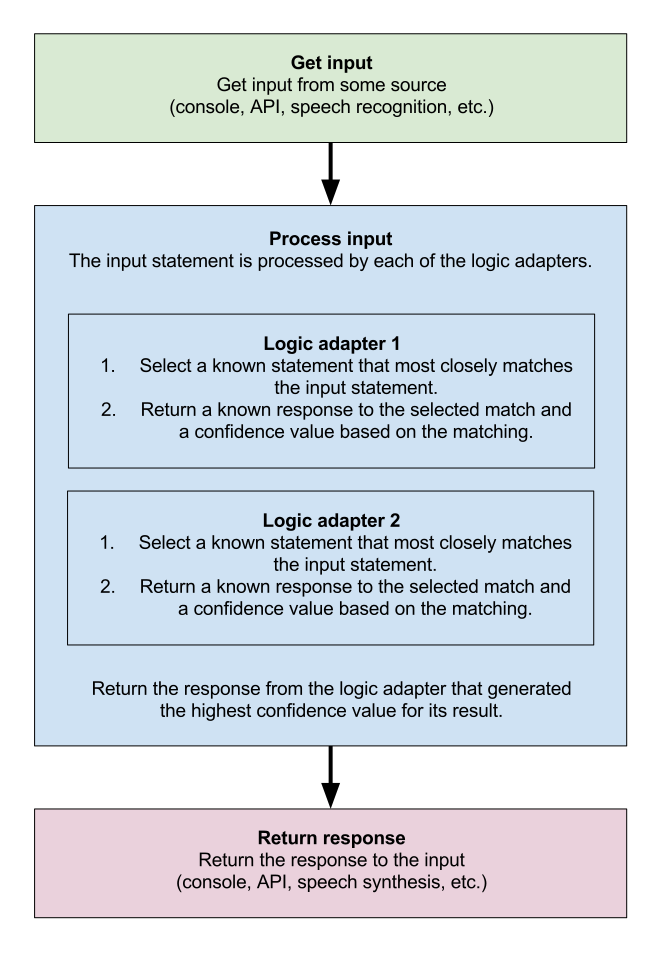
\includegraphics[width=0.6\columnwidth]{chatterbot-process-flow}%
    \caption{\captionstyle{Process flow diagram of how Chatterbot works on a higher level \cite{Chatterbot:online}}}%
    \label{fig:chatterbot-process-flow}%
\end{figure}

Firstly, the user inputs a statement. The statement is then processed by \textit{logic adapters}. A logic adapter is a function which takes text as input, determines whether it can process the input, and generates suitable output.

The main advantage of Chatterbot is its extensibility. While it provides a lot of built-in functionality, it might not be suitable for all projects.

[Add a figure showing how it works in more detail here...]

\subsubsection{Configuration}
Chatterbot provides a \textit{ChatBot} class. A ChatBot object takes several parameters in its constructor which define its behaviour:
\begin{itemize}
    \item \texttt{preprocessors}
    \item \texttt{logic\_adapters}
    \item \texttt{storage\_adapters}
\end{itemize}

\subsubsection{Preprocessors}
The ChatBot instance can take a list of functions in its constructor to be used as preprocessors. Preprocessors can modify the input sent by the user before it is passed to the logic adapters. This is necessary due to the fact that the logic adapters are more likely to perform better if they are given clean input. For example, if the input contains a lot of whitespaces or non-alphanumerical characters, it might be beneficial to remove them. Chatterbot has several preprocessors, however, custom functions can be created and used as preprocessors.

\subsubsection{Logic Adapters}
\textit{Logic adapters} are used to select an appropriate response to a question entered by the user. More than one logic adapter may be used as different types of input may require different processing. For example, Chatterbot by default uses the \textit{BestMatch} logic adapter. However, this adapter is only useful when the question asked has a specific response. If the user asked for the current time, the BestMatch adapter would be unable to answer as there is no specific answer to this question, i.e. the answer changes depending on when the user asks the question. For this reason, a \textit{Time} logic adapter can be created and added to the list of adapters used (Chatterbot has this adapter implemented by default). To help decide which adapter to use if more than one are provided, a custom logic adapter must inherit from the base class \texttt{LogicAdapter} and must implement the method \texttt{can\_process()}. This method is called before the logic adapters generate a response and the user input is passed to it. It must then return True or False based on whether the adapter should process this input or not. \cref{lst:canprocess} shows an example implementation of the \texttt{can\_process} method.

\begin{lstlisting}[caption={\captionstyle{Example implementation of the \texttt{can\_process()} method. Adapted from \cite{Chatterbot:online}.}}, label={lst:canprocess}]
    def can_process(self, statement):
        # If the statements starts with
        # the string 'Hey John',
        if statement.text.startswith('Hey John')
            # it can be processed with this adapter
            return True
        # If not,
        else:
            # it can't
            return False
\end{lstlisting}

This tells the adapter to only process user input which contains the string \enquote{Hey John} (John could be the name of the chatbot) in its beginning.

Another requirement is that custom logic adapters implement the \texttt{process()} method. It takes the input statement as a parameter. Additional response selection parameters can be added if required by the application. An example implementation can be seen in \cref{lst:process}.

\begin{lstlisting}[caption={\captionstyle{Example implementation of the process() method. Adapted from \cite{Chatterbot:online}}}, label={lst:process}]
    def process(self, input_statement, additional_response_selection_parameters):
        import random

        # Randomly select a confidence
        # value between 0 and 1
        confidence = random.uniform(0, 1)

        # For this example,
        # the input will just be returned
        # as output
        selected_statement = input_statement
        selected_statement.confidence = confidence

        return selected_statement
\end{lstlisting}

The \texttt{process()} method must return a \textit{Statement} object. The \textit{text} property of the object should contain the actual response to the input. Additionally, the \textit{confidence} property should be a value between 0 and 1 which indicates how confident the adapter is that this response is correct. In the example above, the text of the output statement is set to the same text that was entered by the user. The confidence value is chosen randomly and the response is returned.

In the event that more than one logic adapters are used, and more than one of them returns a response, the response with the highest value of confidence is selected. If two or more responses have the same value of confidence, then the response of the adapter which is first in the list of adapters is used. \cref{fig:dialog-processing-flow} shows a diagram of response selection with multiple adapters.

\begin{figure}[!htb]%
    \centering
    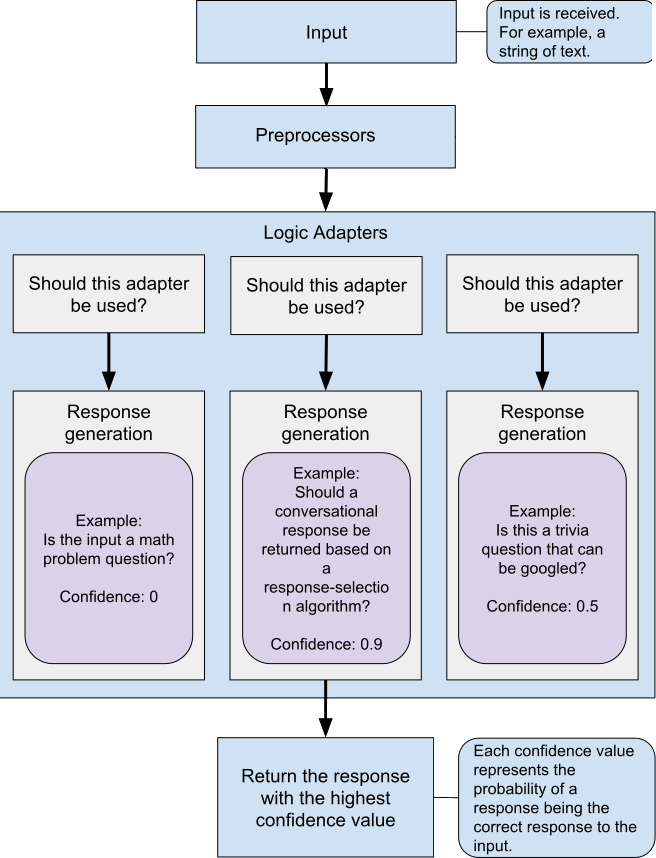
\includegraphics[width=0.7\columnwidth]{dialog-processing-flow}%
    \caption{\captionstyle{Process flow diagram of how responses are selected. Adapted from \cite{Chatterbot:online}}}%
    \label{fig:dialog-processing-flow}%
\end{figure}


By default, Chatterbot has the following adapters included:
\begin{itemize}
    \item Best Match Adapter - used when question that have a specific response are asked. This requires training data and the quality of the response depends on the quality of the training data. The adapter uses a specific \textit{similarity} function to search through the known questions. When it finds the most similar one, it then returns the known response to this question. The similarity functions available by default are:
        \begin{itemize}
            \item Levenshtein Distance - this method is used by default...
            \item Jaccard Similarity - ...
            \item Sentiment Comparison - ...
            \item Synset Distance - ...
            \item Custom similarity functions may be implemented if needed.
        \end{itemize}
    \item Time Logic Adapter - allows the user to ask about the current time.
    \item Mathematical Evaluation Adapter - calculates mathematical expression the user has entered.
    \item Specific Response Adapter - returns a specific predefined answer to a specific statement configured in the adapter.
\end{itemize}

\subsubsection{Storage Adapters}
\textit{Storage Adapters} are an interface for Chatterbot to connect to different storage technologies \cite{Chatterbot:online}. The storage adapter used by default is the \textit{SQL Storage Adapter}. It allows the chatbot to store its data in a local \textit{SQLite} relational database. The structure of the database can be seen in \cref{fig:db-schema}.

\begin{figure}[!htb]%
    \centering
    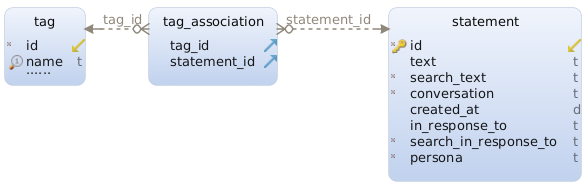
\includegraphics[width=0.9\columnwidth]{db-schema}%
    \caption{\captionstyle{Diagram of the database schema.}}%
    \label{fig:db-schema}%
\end{figure}

[Explain the structure here....]

\subsubsection{Training}
ChatterBot includes tools that help simplify the process of training a chatbot instance. ChatterBot’s training process involves loading example dialogue into the chatbot’s database. This either creates or builds upon the graph data structure that represents the sets of known statements and responses. When a chat bot trainer is provided with a data set, it creates the necessary entries in the chatbot’s knowledge graph so that the statement inputs and responses are correctly represented. An example of this can be seen in \cref{fig:training-graph}.

\begin{figure}[!htb]%
    \centering
    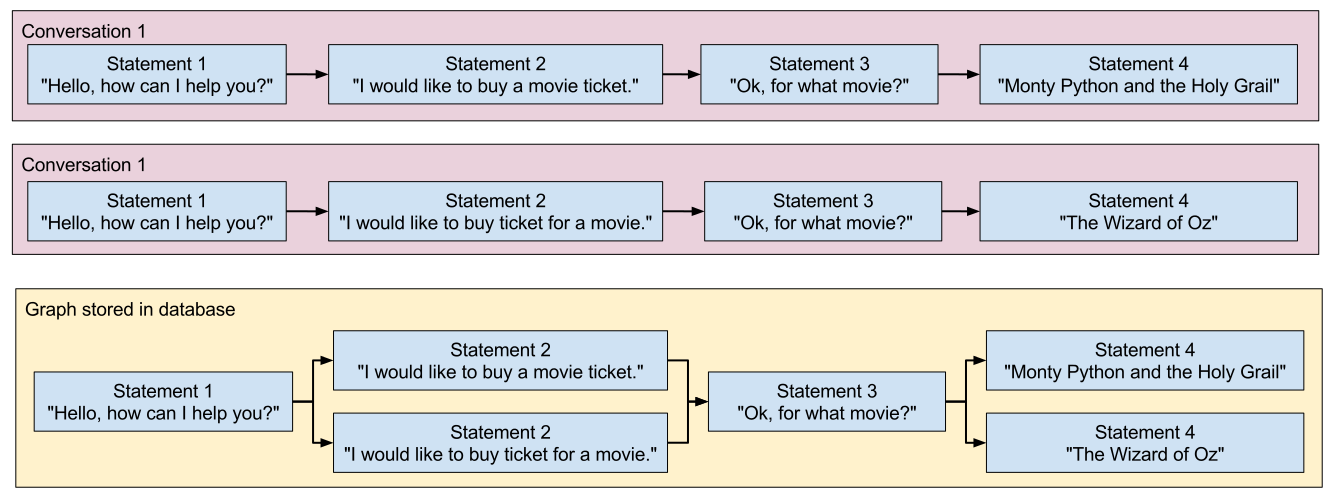
\includegraphics[width=1.0\columnwidth]{training-graph}%
    \caption{\captionstyle{Example of a training graph \cite{Chatterbot:online}.}}%
    \label{fig:training-graph}%
\end{figure}

[talk about how words are tagged with nltk here]

Chatterbot includes the following training clasess by default:
\begin{itemize}
    \item List Trainer - allows a chat bot to be trained using a list of strings where the list represents a conversation.
    \item Corpus Trainer - allows the chat bot to be trained using corpus data stored in an external file.
    \item Ubuntu Corpus Trainer - allows chatbots to be trained with the data from the Ubuntu Dialogue Corpus.
\end{itemize}

New training classes may be created and used to train a chatbot. The custom trainer must inherit from the \textit{Trainer} class and must implement the methods \texttt{train()} which can accept any arguments.

\subsubsection{Statements}
ChatterBot’s statement objects represent either an input statement that the chat bot has received from a user, or an output statement that the chat bot has returned based on some input.

ChatterBot stores knowledge of conversations as statements. Each statement can have any number of possible responses.

\begin{figure}[!htb]%
    \centering
    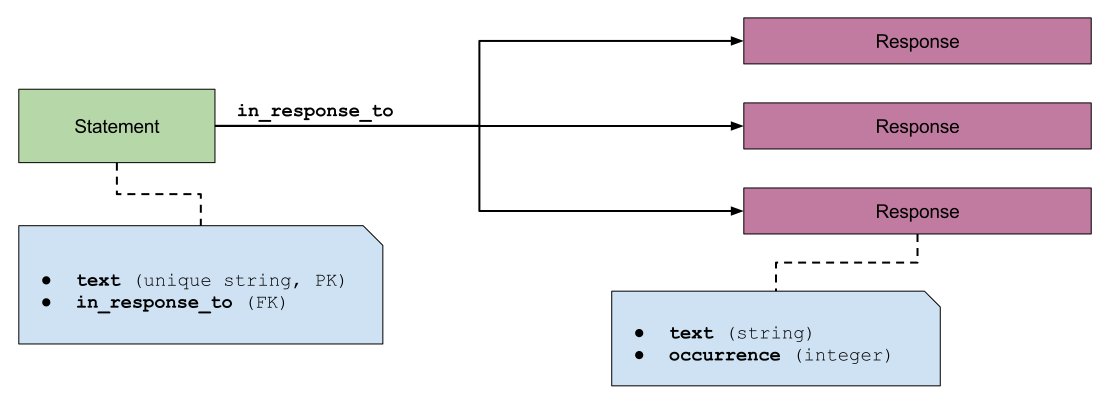
\includegraphics[width=1.0\columnwidth]{statement-response-relationship}%
    \caption{\captionstyle{Statement-response relationship \cite{Chatterbot:online}.}}%
    \label{fig:statement-response-relationship}%
\end{figure}

Each Statement object has an in\_response\_to reference which links the statement to a number of other statements that it has been learned to be in response to. The in\_response\_to attribute is essentially a reference to all parent statements of the current statement.

\begin{figure}[!htb]%
    \centering
    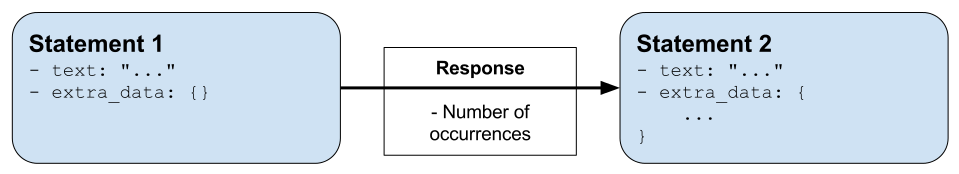
\includegraphics[width=1.0\columnwidth]{statement-relationship}%
    \caption{\captionstyle{Statement relationship \cite{Chatterbot:online}.}}%
    \label{fig:statement-relationship}%
\end{figure}

The count of recorded statements with matching, or similar text indicates the number of times that the statement has been given as a response. This makes it possible for the chat bot to determine if a particular response is more commonly used than another.

\subsection{Python}
According to [ref needed] the most used languages in the field of AI are:
\begin{itemize}
    \item Python
    \item Java
    \item C++
\end{itemize}

While each of these languages could be a viable option, there seems to be an agreement that \textit{Python} is the most popular choice.  The reason for this is that Python has a very large number of libraries. Furthermore, it is one of the most popular languages for AI-related programming. Libraries like \textit{nltk, numpy, pytorch, tensorflow}, etc. are widely adopted and actively developed to allow programmers to utilise the latest findings in AI research. Additionally, Python is known to greatly reduce development time as it provides a lot of \enquote{syntactic sugar} and automatic garbage collection. In traditional programming languages such as \textit{C++}, etc. manual memory management is an issue for new programmers and security and performance issues might occur when it is not implemented correctly. 

Python is a weakly-typed language, which means that variable types are deduced by the python interpreter. For this reason, developers do not have to specify the type of variable they are declaring. However, this could lead to problems as the programmer has to remember what type of data each variable is storing and has to be careful not to assign a different type of value to it as that would cause errors. Furthermore, Python is a high-level language, meaning that it provides more layers of abstraction. This results in the writing of less code to solve a specific problems. This is even more true when libraries (also referred to as \textit{modules}) are taken into account. Python has an enormous selection of modules - 169515 according to the official python package repository \cite{PyPI:online}. Additionally, Python is a multi paradigm language, i.e. it supports object-oriented programming, functional programming, imperative programming and procedural programming. Lastly, it is a cross platform language, being able to run on most major operating systems.

Similarly to other programming languages, Python does have disadvantages. The main one is that it is an \textit{interpreted} language. This means that rather than converting the code written by a programmer to an executable file (bytecode, CPU instructions), the python interpreter reads it line by line and executes the instructions. Another problem caused by this is that errors can only be found during the execution of a program. If some part of the program never gets executed, potential errors might not be found as the interpreter never reads those lines of code. This issue can be solved relatively easily. For example, unit tests can be written which execute all functions of a program. Even though this problem doesn't exist with languages such as C++, where errors are reported during compilation, programs still have to be tested for logical errors.

\subsection{Flask}
The decision to create a website for the front-end of the project instead of a desktop or mobile application was made. This allows the application to be used from any device, desktop or mobile. 

Flask is a microframework for Python used for website development. It is called a microframework as it aims to only include the core functionality required to create a website. This means developers are not forced to use a specific technology chosen for them by the Flask developers. Instead, many extensions exist which provide specific functionality. For instance, by default, Flask does not include any database....

Flask uses several python libraries to achieve its functionality. A description of each one is provided below:

\subsubsection{Jinja}
Jinja is Python template engine...

\subsubsection{Twitter Bootstrap}
The goal was to implement a website which could be used from any device which can access websites. To ensure that the website worked well on mobile and desktop devices, Twitter Bootstrap was used. It is a CSS framework which enables the creation of websites with a responsive design. That is, the layout of the website elements changes based on the screen size of the device used to view the website. This is achieved through bootstrap's grid system.

\subsection{Pytest}
Pytest is a unit test framework for Python...

\newpage
\section{Implementation}\label{sec:impl}
\subsection{Version control}
The first decision made when starting to implement the application was to use \textit{Version Control}. The version control system used was \textit{Git} and the code was hosted in a \textit{GitHub} repository. The reason for this was personal preference and previous experience with these technologies. 

Using Git and Github meant that the source code of the application could be easily shared between computers. Additionally, changes between versions of the program could be tracked. In the event that issues arose, the application could be reverted to a previous working version. 

Another feature of Git and Github used was \textit{branches}. Branches allow for having several versions of the code at the same time:
\begin{itemize}
    \item Master branch - stable version of the application which can be deployed.
    \item Dev branch - the most recent updates to the application which might not be fit for deployment. It can be updated until it is considered stable enough. It can then be merged into the master branch and deployed.
    \item Feature branches - a branch where a specific feature is implemented. It can then be merged into the development branch.
\end{itemize}

Using branching proved to be beneficial as... 

\subsection{Testing}
Since the application consisted of many different components communicating with each other, problems were often encountered during the development process. For example, the chatbot expects to find the training data in a specific location. Therefore, the web crawler has to store the data in this exact location. To ensure changes would not break the current functionality, unit tests were implemented with the Python library PyTest. 

The first set of unit tests written was for testing the command line interface. Many modifications and updates were made to the web crawler during the development process. This always resulted in problems with the command line interface functionality as most of the commands modify the output of the crawler. The unit tests for the command line interface tests each one of the commands in order.

The second set of tests was for the chatbot functionality. These tests use PyTest fixtures which set up the necessary conditions before the tests are executed and delete any files or data left after they are run. These tests ensure the output produced by the chatbot is correct. 

The last set of unit tests implemented was for the storage adapter used. 

\subsubsection{Code Coverage}
The PyTest library supports extensions. One such extension is pytest-cov which generates code coverage reports. Code coverage is a metric used to specify how many lines of code are executed when unit tests are run. For example, a code coverage of 100\% means that all of the code in the project is tested. Therefore, the higher the code coverage, the better. 

The pytest-cov coverage reports show detailed information about each file in the program that is tested. The code coverage for each file is shown alongside the missed lines of code. At the end of the report, the average code coverage is shown. An example report can be seen in \cref{lst:codecov}.

The aim for this project was to achieve a code coverage of at least 80\%, which was accomplished. Since a lot of libraries were used, it was impossible and infeasible to test all of the code in the project. It was assumed the creators of libraries have tested their code thoroughly. What is more, most libraries provide their own tests which prove that the code works.

\begin{minipage}{\linewidth}
    \begin{lstlisting}[caption={\captionstyle{A code coverage report produced with pytest-cov.}}, label={lst:codecov}]
    Name                   Stmts   Miss  Cover
    ------------------------------------------
    chatbot/__init__.py       49     24    51%
    chatbot/bot.py            86      9    90%
    chatbot/config.py          3      0   100%
    chatbot/constants.py      22      0   100%
    chatbot/crawler.py        80      6    92%
    chatbot/logic.py          69     13    81%
    chatbot/models.py         29      1    97%
    chatbot/run_it.py          2      0   100%
    chatbot/storage.py       199     51    74%
    ------------------------------------------
    TOTAL                    539    104    81%    
    \end{lstlisting}
\end{minipage}

\subsection{Continuous Integration \& Deployment}
\subsubsection{Continuous Integration}
A Continuous Integration service could be used to automatically execute the unit tests to no issues have occured. Changes were made to the project daily, however running the tests after each change was time consuming. Using Continuous Integration meant that every time a commit was pushed to the GitHub repository, the tests would be run automatically, and any issues would be found quickly. Furthermore, since branches were used, the tests could be run after merging changes into the main branch. This allowed for the discovery of integration problems.

The Continuous Integration service used was Travis CI due to personal preference and previous experience. It is used for continuous testing and delivery of projects hosted on GitHub. To set it up, the GitHub account which owns the project repository was linked to Travis CI and access was given to it to read the repository. Travis CI can be configured by adding a “.travis.yml” configuration file in the root directory of the repository. The file is written in the YAML format. Firstly, the operating system used to compile the project is specified. In this case \texttt{Ubuntu 16.04 (Xenial Xerus)} is used. Additionally, the language of the program is specified, i.e. Python. The versions of the language can be specified next. In this case, the project is tested with Python 3.6 and 3.7 which are the currently latest versions. Travis CI also supports the following steps:
\begin{itemize}
    \item \texttt{install} – this step is executed before the testing happens. It is used to install any packages that are not installed on Ubuntu by default. In this case, there are no packages that should be installed, however the libraries used in the project are downloaded. Using the package manager, pip, all libraries are downloaded.
    \item \texttt{before\_script} – this step occurs before the test script is executed. It is used to set the environment variables Flask expects. 
    \item \texttt{script} – this step executes the command which runs the unit tests. In this case, it is the \texttt{pytest} command. No other setup is required as pytest is able to discover unit tests without any additional configuration. However, since code coverage reports can be generated, the optional parameter \texttt{--cov} is added so that a coverage report is created.
    \item \texttt{after\_success} – this step is only executed after the tests are completed if they have completed successfully. The coverage report generated in the previous step is uploaded to codecov.io. It can then be inspected in detail. Codecov.io provides in-depth reports and charts of code coverage. Each file in the repository can be seen and it is shown whether each line is tested. This is useful for finding possible problematic areas which are not tested. 
    \item \texttt{cache} – this option specifies dependencies or folders which do not change often. They can be stored, instead of being downloaded every time the build process is run. In this case, the pip dependencies can be cached which speeds up the testing process as the libraries do not have to be downloaded every time.
\end{itemize}

\subsubsection{Continuous Deployment}
Since the website was hosted on Python Anywhere and the master branch of the GitHub repository contained the release version of the code, Continuous Deployment could be implemented. This was done for faster deployment every time code was added to the master branch. This had to be implemented manually since neither Python Anywhere nor Travis CI had any methods of deploying Flask websites. 

The first step was to create an end point in the website. It was created at “/webhook”. It’s purpose was to receive requests from GitHub. GitHub has a feature called “webhooks”. It allows its users to send a request to any end point every time a specific event occurs in the repository. For example, it can be configured to send a request when there has been a commit. This is exactly what it was used for. Every time there are new changes in the master branch, the webhook send a request to the live website’s “/webhook” end point. The website is configured to inspect the request body when it receives a request. It is checked whether the event that occurred is a commit and whether the commit was made to the master branch. If this is the case, changes from the repository can be pulled directly. This was achieved with the Python library GitPython. Unfortunately, when changes are made to the website, Python Anywhere requires the site owner to reload the website. This has to be done manually by going to the site settings and pressing a \enquote{reload} button. Python Anywhere has an API which provides an end point for reloading a website remotely, however, this cannot be done from the same program that runs the server as the request times out due to the server going offline for reloading. 

\subsection{Development Tools}
Used PyCharm IDE, virtual environments, pip, terminals, etc...

\subsection{Application}
Early in the development process it became clear that the application should consist of two main parts: the back-end and the front-end. The back-end program processes the user input and generates suitable output. The front-end is the program the user interacts with. It allows them to send a message to the chatbot and receive an answer.

\subsection{Back-end}
The back-end program consists of a web crawler and the chatbot program. The web crawler is used to collect training data from Stack Overflow, while the chatbot programm processes the user input to generate a suitable response to their question.

\subsubsection{Web Crawler}\label{subsub:crawler}
Firstly, before creating the back-end program, it was necessary to collect training data for the chatbot. This could be achieved in many different ways, however the decision to scrape \footnotemark[1] the website Stack Overflow was ultimately made. Stack Overflow is one of the most popular websites where programmers can ask questions about numerous programming languages and technologies. Furthermore, there is a voting system which sorts the answers by number of votes. Additionally, the person who asks a question is able to mark a specific answer as the \enquote{accepted answer}. This meant that when collecting data, the answers to each question could be sorted by number of votes, and the \enquote{accepted answer} could be used as the default answer. Unfortunately, some questions have no accepted answer or no answers at all. Despite that, Stack Overflow has a wealth of information and proved to be a good source.

\fancyfootnotetext{1}{Web scraping - a technique for extracting data from a website.}

Another option for data collection was the numerous websites which provide beginner information about a specific language. However, as described below, supporting web crawling of different websites could be a difficult task due to the different structure of each website. Furthermore, these websites had a limited amount of information and some of them had outdated or low-quality information.

The last consideration for data collection was using books as training data. There exist numerous books about programming and they contain detailed information about technologies. However, it was decided that using books was infeasible as the Chatterbot library required training data in the format question - answer. Converting a book to this format would require creating a another program which would possibly utilise NLP and other advanced machine learning techniques. This would be a difficult task and it would be outside of the scope of this project.

It was decided that data about the C++ programming language would be collected. C++ is widely used for programs where performance is most important such as games. However, it is known to have a steep learning curve....

A python program was written to collect data from Stack Overflow. The Python module \textit{BeautifulSoup} was utilised to achieve data extraction from the pages. The program expects the following variables to work:
\begin{itemize}
    \item Starting page - the first page to be crawled.
    \item Number of pages to be crawled
\end{itemize}

Initially, they were implemented as constants, however it was planned for them to be set with command line arguments later.

Another variable, \texttt{current\_page} (indicating the currently scraped page,) is initially set to the value of the starting page variable. Then a \texttt{while} loop is executed until the value of \texttt{current\_page} becomes the same as the value of \texttt{start + num\_pages}, where \texttt{start} is the starting page and \texttt{num\_pages} is the number of pages to be crawled. The value of \texttt{current\_page} is incremented by one at the end of each loop iteration. In the beginning of each loop iteration, a URL of the page to be scraped is generated. This is achieved by appending several \textit{GET} parameters to the base Stack Overflow URL. The structure of a Stack Overflow URL can be seen in \cref{fig:so-url}.

\begin{figure}[!htb]%
    \centering
    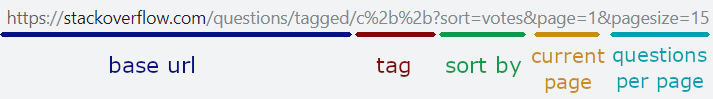
\includegraphics[width=1.0\columnwidth]{so-url}%
    \caption{\captionstyle{The structure of a Stack Overflow URL.}}%
    \label{fig:so-url}%
\end{figure}

The \textbf{base URL} is a constant value. The \textbf{tag}, \texttt{c\%2b\%2b}, is used to show only questions categorised under this tag. In this case, \textbf{C++} questions are requested as \texttt{\%2b} expands to the symbol \texttt{+}. However, the tag can be changed to any language or technology. For instance, to collect data about Java, the tag can be changed to \texttt{java} and this would result in only extracting data from Java-related questions. The \textbf{sort} parameter indicates the order in which the questions are shown. In this case sorting by \texttt{votes} results in the most upvoted questions being shown first. The \textbf{page} parameter indicates the current page. Since there is a large number of questions on the website, it is impossible to display them all in one page. For this reason, questions are split into pages. The last parameter used is \textbf{pagesize}. It indicates how many questions should be shown per page. To generate a URL, all the parameters are appended to the base URL, and the \textbf{page} parameter is dynamically generated based on the \texttt{current\_page} variable. 

With the generated URL, a \textit{request} can be sent to Stack Overflow. Using the Python library \textbf{requests}, a GET request can be sent. The returned result is the source code of the page that the request was sent to. Data can now be extracted from the source code using the \textit{Beautiful Soup} Python library. Firstly, an instance of the \texttt{BeautifulSoup} class is created. The source code retrieved earlier is passed to it. The library can then parse the code and create a \textit{parse tree} from which data can be extracted. The data needed from each page of questions is the hyperlink to each question's page. To extract this data, the method \texttt{find\_all()} of the \texttt{BeautifulSoup} object can be used. It returns a list of all the occurrences of a specified HTML tag as a parameter. In this case, the HTML \texttt{<a>} tag is needed as it is used to create hyperlinks. However, there are numerous hyperlinks on each Stack Overflow page. Only the hyperlinks which lead to a question page are needed. Using the Chrome browser developer tools, it was discovered that each link to a question was assigned a class of "question-hyperlink". \cref{lst:hyperlink} shows the code of an example hyperlink to a question.

\begin{lstlisting}[language=html, caption={\captionstyle{An example hyperlink to a Stack Overflow question.}}, label={lst:hyperlink}]
    <a href="/questions/121162/what-does-the-explicit-keyword-mean" class="question-hyperlink">What does the explicit keyword mean?</a>
\end{lstlisting}

With this information, only the URLs of the questions could be extracted. \cref{lst:extract-questions} shows the source code for extracting the hyperlinks to each question.

\begin{lstlisting}[caption={\captionstyle{Extracting the URL of each question on a Stack Overflow page.}}, label={lst:extract-questions}]
    # get a link to each question
    for ques_link in soup.find_all('a', {'class': 'question-hyperlink'}):
        # make sure no extra links are crawled
        if q_no == PAGE_SIZE:
            break
        # generate the link
        url = SO_URL + ques_link.get('href')
        # print question title for debugging purposes
        title = ques_link.get_text()
        if VERBOSE_OUTPUT is True:
            print(title)
        # parse this question
        parse_question(url, title, data)
        # keep track of current question number
        q_no += 1
\end{lstlisting}

The \texttt{find\_all()} method on line 3 returns a list of all \texttt{<a>} tags with a class parameter set to "question-hyperlink". A for-each loop iterates through this list. Each hyperlink's destination is extracted from the \texttt{href} parameter using the \texttt{get()} method. Each link's text is also extracted using the \texttt{get\_text()} method. The destination URl, however, is incomplete and it needs to be appended to the base Stack Overflow URL. The final question URL and the question title are passed to the \texttt{parse\_question()} method. The if-statement on line 4 is needed as there is a "Hot Network Questions" section on each Stack Overflow page which contains hyperlinks to popular questions. The if statement ensures that only the required number of question links are scraped.

The \texttt{parse\_question()} method can be seen in \cref{lst:extract-answers}.
\begin{lstlisting}[caption={\captionstyle{Extracting answers for a specific Stack Overflow question.}}, label={lst:extract-answers}]
    def parse_question(url, title, data):
    # page to be scraped
    page = requests.get(url, headers=headers, timeout=(3, 30))
    # initialise bs4
    soup = BeautifulSoup(page.content, 'lxml')
    # get the question data, contained in a <div> with class "postcell"
    question = soup.find('div', class_='postcell')
    if question is not None:
        answers = soup.find_all('div', class_='answercell')
        # limit to max 3 answers per question
        end = len(answers)
        if end > CRAWLER_NUM_ANSWERS:
            end = CRAWLER_NUM_ANSWERS
        # for each answer found
        for i in range(0, end):
            # get the answer text
            answer = answers[i].find('div', class_='post-text').extract()
            # store the question and the answer in their own list
            answer = str(answer)
            entry = [title, answer]
            # add to the main list
            data.append(entry)
\end{lstlisting}

The \textit{requests} library is used again to send a GET request to each of the question pages. The returned source code is then passed to an instance of \texttt{BeautifulSoup}. Using the Chrome browser's development tools it was discovered that the data about a question is stored in a HTML \texttt{<div>} with a class value "postcell". However this includes all data including the date the question was asked, the author, etc. The actual text of the post is stored in a \texttt{div} with class value "post-text". Each answer is stored in a \texttt{<div>} with class value "answercell". The actual text of the answer is stored in a \texttt{<div>} with class value "post-text". With this information, the answers to each question can be extracted by first finding them with the \texttt{find\_all() method}. The resulting list is then iterated through and each answer's text is extracted. The maximum number of answers scraped is currently set to three. However, the if statement on line 12 ensures that in the event that less than three answers exist, no errors occur. Lastly, the question title and the top three answers are stored in a Python \textit{dict}.

The last step is to save the data stored in the dict to a file. The ChatterBot library supports training from external files by default. Custom trainers can be created to support different file formats, however the \textit{YAML} format which is supported by default can be used. The structure of a training file can be seen in \cref{fig:yaml-train}. 

\begin{figure}[!htb]%
    \centering
    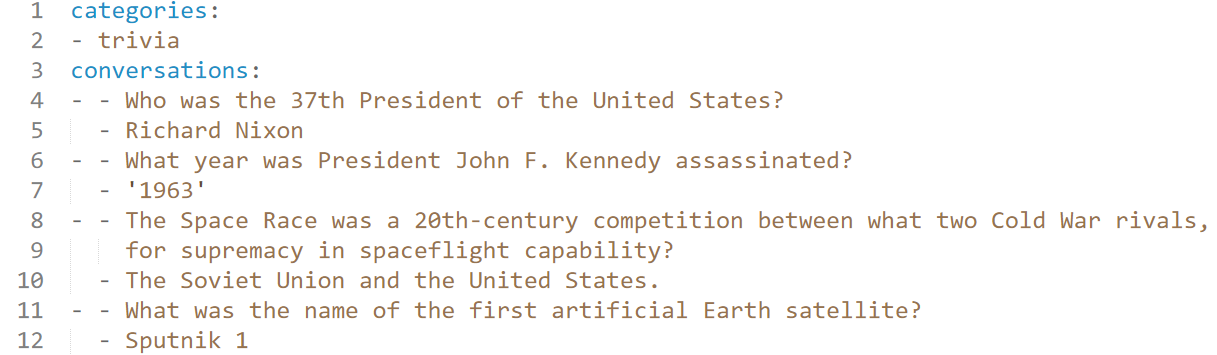
\includegraphics[width=1.0\columnwidth]{yaml-train}%
    \caption{\captionstyle{Example training file in the YAML format.}}%
    \label{fig:yaml-train}%
\end{figure}

The "\verb|- -|" tag is used to signify a statement, while the "\verb|-|" tag signifies an answer to a statement. To save the data collected from Stack Overflow in this format, the \textit{Ruamel.YAML} Python library was used. To ensure the data was saved in this required format, however, it had to first be stored in an appropriate data structure. Each question - answer pair was stored in a Python list. Each list was appended to a Python dict. Using the Ruamel.YAML library's \texttt{yaml} class, the data could be simply written to a file using the \texttt{yaml.dump()} method. The code used to achieve this can be seen in \cref{lst:write-file}.

\begin{lstlisting}[caption={\captionstyle{Writing scraped data to a file in the YAML format.}}, label={lst:write-file}]
# initialise yaml library
yaml = YAML()
yaml.default_flow_style = False
# create output file
out_file = os.path.join(DATA_DIR_PATH, "training_data.yaml")
# open out file
with open(out_file, 'w+', encoding="utf-8") as outfile:
    # write data
    yaml.dump(final_data, outfile)    
\end{lstlisting}

Even though the resulting program worked well, it was slow as only one question was processed at a time. To improve its performance, multithreading was implemented.

\begin{lstlisting}[caption={\captionstyle{Multithreaded optimisation of the web crawler.}}, label={lst:threads}]
    func = partial(crawl_pages, num_pages)
    try:
        with ThreadPoolExecutor(max_workers=workers) as executor:
            for i in range(workers):
                executor.submit(func, (i * num_pages + 1))
    except (KeyboardInterrupt, EOFError, SystemExit):
        print("Interrupted...")
\end{lstlisting}

\subsubsection{Chatbot}
The other main part of the back-end program is the Chatbot object instance. The initialisation of the chatbot can be seen in \cref{lst:chatbot}.

\begin{lstlisting}[caption={\captionstyle{Initialisation of the Chatbot object.}}, label={lst:chatbot}]
bot = ChatBot(
    "C++ bot",
    storage_adapter="chatterbot.storage.SQLStorageAdapter",
    preprocessors=[
        'chatterbot.preprocessors.unescape_html'
    ],
    logic_adapters=[
        {
            'import_path': 'chatbot.logic.BestMatch',
            'default_response': 'I am sorry, but I do not understand.',
            'maximum_similarity_threshold':  0.90
        }
    ]
)
\end{lstlisting}

The first argument passed to the constructor, the string "C++ bot", is the name of the chatbot. It can be useful when there are multiple chatbots created, however in this case there is only one chatbot instance. The second argument, \texttt{preprocessors} is a list of the preprocessors the chatbot should use when it receives user input. The \texttt{unescape\_html} preprocessor is included in chatterbot. It converts escaped HTML characters into unescaped HTMl characters. For instance, "\texttt{\&lt;b\&gt;}" is converted to the \texttt{<b>} tag. This preprocessor has to be used as the data collected from Stack Overflow includes HTML tags and some of them are escaped.

The next argument passed is a list \texttt{logic\_adapters}. The adapters used in this case are a BestMatch adapter and a SpecificResponse adapter.

The last argument is the \texttt{database\_uri}. An SQLite database is used and the value of the parameter is the name of the file where the database is stored.


\subsection{Front-end}
The front-end was implemented in Python with the Flask module.

\subsubsection{Project Structure}
As suggested in the Flask documentation \cite{Flask:online}, the project was structured in the following way: 
\begin{Verbatim}[frame=single]
Chatbot/
|---requirements.txt
|   
|---chatbot/
|   |---__init__.py
|   |---constants.py
|   |---crawler.py
|   |---bot.py
|   |   
|   |---static/
|   |   |---css/
|   |   |   |---style.css
|   |   |       
|   |   |---js/
|   |       |---chatbot.js
|   |           
|   |---templates/
|           |---base.html
|           |---chatbot.html
|           
|---tests/
|---venv/    
\end{Verbatim}

The root folder of the project is the \texttt{Chatbot/} directory. It contains the \texttt{chatbot/} directory in which the Python code for the back-end program is stored. The \texttt{static/} directory contains the static files used in the website - the CSS styles and the javascript code as well as any images that might be used. The \texttt{tests/} directory contains the unit tests for the application. Lastly, \texttt{venv} contains the Python \textit{virtual environment} used for the project. Structuring the project this way ensures that the different .... are separated and organised.

\subsubsection{Application Setup}
The Flask documentation recommends organising the code in modules. For this reason, the \texttt{\_\_init\_\_.py} file is placed in the \texttt{chatbot/} directory. This tells the Python interpreter that chatbot is a module which can be imported in Python files. Additionally, the \texttt{\_\_init\_\_.py} file defines a method which initialises an instance of the \texttt{Flask} class. This method is known as the \textit{Application Factory} \cite{Flask:online}. The initialisation of the Flask app is achieved as follows:

\begin{enumerate}
    \item An instance of the Flask class is created.
    \item The Flask instance is configured. A \texttt{SECRET\_KEY} variable is required by Flask. It is used for encryption of sensitive data such as passwords. During development, its value is set to the string "dev" so that debuggers can read encrypted information.
    \item The pages of the Flask application are initialised. The code for creating the home page can be seen in \cref{lst:homepage}. On line 1, the address of the page is specified. The "/" indicates that this is the home page and is shown by default when the website is accessed. If a Contact page were to be added, its location would be "/contact" and it would be accessed by navigating to the address \texttt{example.com/\textbf{contact}}. Line 2 defines a Python function which will be called when this address is accesed. Line 3 uses the Flask method \texttt{render\_template()}. It requires the name of an HTML file which will be shown when this page is accessed. The HTML file is stored in the \texttt{templates/} directory. This method takes any number of other optional arguments. Every other variable passed to it will be passed to the template specified and its value can be used via the Jinja templating language. In this case, a 'title' variable is passed which specifies the title that will be shown in the page.
    \item The last thing Flask requries is that the Application Factory returns the initialised and configured Flask object.
    \item The website can be run using the default server that comes with Flask. To do this, the command \texttt{flask run} can be executed from a terminal. Flask uses environment variables to locate a project. The variable \texttt{FLASK\_APP} must be set before running the server. To run the server in debug mode, the variable \texttt{FLASK\_ENV} may be set to "development". 
\end{enumerate}

\begin{lstlisting}[caption={\captionstyle{Initialisation of the home page of the Flask application.}}, label={lst:homepage}]
@app.route("/")
def home():
    return render_template("chatbot.html", title="Chatbot")
\end{lstlisting}

\myparagraph{Website Design}
The website consists of a single page which resembles a text messaging application. The main goal was to create a clean and simple interface which is easy to use and feels familiar. Messaging apps such as Facebook Messenger and WhatsApp were used as reference. The website interface is shown in \cref{fig:site-interface}.

\begin{figure}[!htb]%
    \centering
    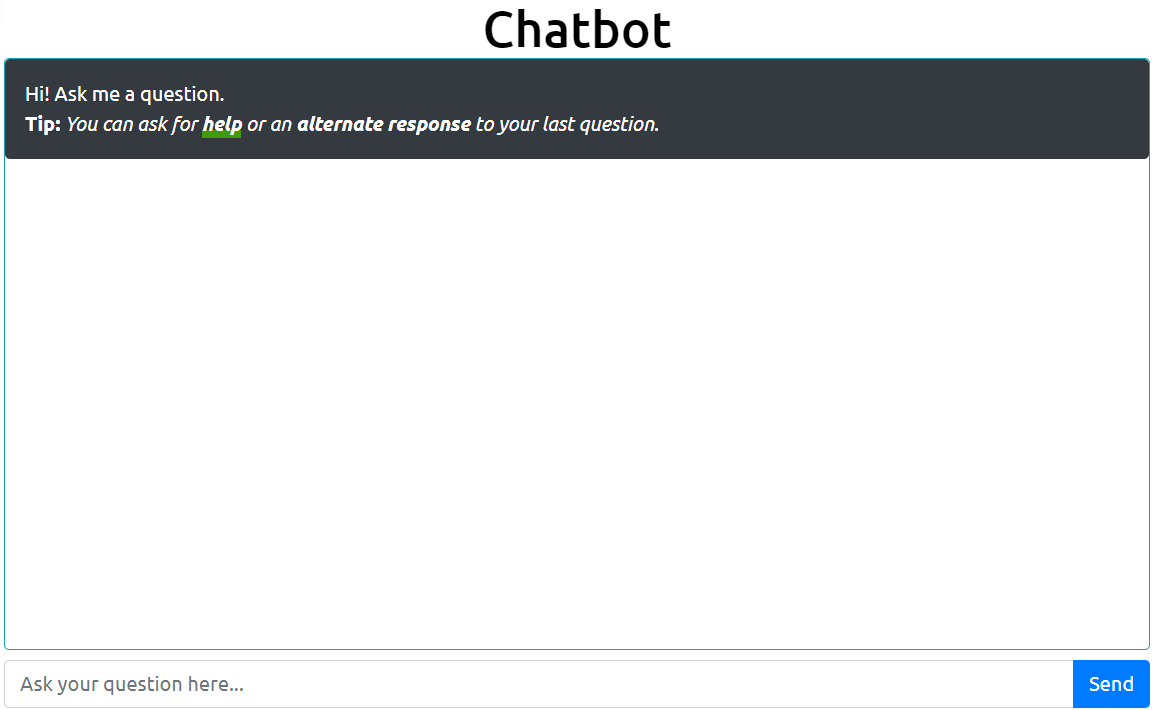
\includegraphics[width=1.0\columnwidth]{app-interface}%
    \caption{\captionstyle{The interface of the website.}}%
    \label{fig:site-interface}%
\end{figure}

The elements that can be seen on the figure were created using HTML and Jinja templates. A main template (\texttt{base.html}) contains the elements that exist on every page of the website - the page title and the window title. All the HTML code used to create a page is stored in the \texttt{<html>, <head>, and <body>} tags. In its \texttt{<head>} tag all the css styles and javascript scripts are loaded. Additionally, the \texttt{<title>} tag is used with a value passed from Application Factory. The \texttt{<body>} tag only contains an HTML \texttt{<h1>} tag which has the value of the variable title passed from the Python code. The code used to achieve this can be seen in \cref{lst:jinjavar}. The code on line 1 checks if the variable \texttt{title} has a value. If it does, it is used on line 2 as a heading. There is no other content in the \texttt{<body} tag, except for a Jinja block. It defines a place in the page where content can be inserted. This can be achieved by creating another template which extends the base template and implementing the block content in it.

\begin{lstlisting}[caption={\captionstyle{Using a variable passed from Python in a Jinja template.}}, label={lst:jinjavar}]

    <h1>{{ title }}</h1>

\end{lstlisting}

A specific template for the home page, \texttt{chatbot.html}, implements the elements specific to the chatbot page: the chatbox, the text field and the Submit button. It extends the \texttt{base.html} template. This means that all the code in the base template will be copied in the chatbot template. By defining a block with the same name as the block in the base template, the content of the chatbot page can be implemented.

The styling of the website was achieved using CSS. The CSS framework \textit{Bootstrap 4} by Twitter was used to style the website and to ensure that it can be viewed on devices with different screen sizes with no issues. Bootstrap's responsive design allows for positioning elements in a grid of rows and columns. Each row can contain up to twelve columns. When the page is resized, the columns are re-ordered and their size is changed dynamically to fit the page. The font size and can also change dynamically so that it is readable at different resolutions. 

Although Bootstrap does not require any specific setup or configuration, the Flask extension Bootstrap-Flask can be used to implement a bootstrap layout more easily. It creates Jinja macros such as \texttt{bootstrap.load\_css()}, \texttt{bootstrap.load\_js()} which are automatically replaced with the required stylesheets and javascript which Bootstrap uses.

The chatbot page consists of three rows with one column per row. Custom CSS was written so that the different elements have appropriate size. The title is positioned at the top of the page and the text input box and the button are positioned at the bottom. The chatbox is in the center of the page and it occupies all the remaining free space. By default, Bootstrap uses rows with the same height. However, custom css was created to position the elements more precisely and to change their height. To ensure the responsive design still worked, the appropriate CSS units were used. Instead of giving elements a specific height, e.g. "20 pixels", relative units such as \texttt{\%} and \texttt{vh} (viewport height) were used.

\subsection{Back-end and Front-end Communication}
The communication between the front-end and the back-end is required as the user input has to be sent to the back-end program for processing. When the input is processed, the resulting output has to be sent back to the front-end. This communication was achieved with the Javascript language. 

JavaScript is a client-side programming language which runs inside web browsers. It can be used to dynamically change a website's content, store information and handle requests and responses. The JQuery library was used as it provides wrappers around JavaScript functions which allow for writing of less code to achieve the same functionality.

Firstly, the JavaScript program handles user input. Using JQuery event handlers, it is waited for a click on the Send button or the Enter keyboard key to be pressed. When either of these events occurs, the text stored in the text input field is stored in a variable. This variable is then passed to another method which forwards it to the back-end program. Before that, the input is checked. For instance, if the user hasn’t entered any text, they are shown an error message. After it has been confirmed the input is valid, a GET request is sent to the server (the back-end program). The data is sent in the JSON format. The only data required for a regular user question is the user input. An example of data sent in the JSON format can be seen in \cref{lst:regularreq}. Javascript supports asynchronous get requests, therefore the request can occur in the background without affecting the responsiveness of the page. To let the user know that the program is processing their input, a loading animation is displayed. When the request is completed and a response has been returned by the back-end program, the loading animation is hidden and the response is added to the chatbox.   

\begin{lstlisting}[caption={\captionstyle{Example data sent to the back-end for processing in the JSON format.}}, label={lst:regularreq}]
{
    "request_type": "regular",
    "message": "Hi, how are you?"
}
\end{lstlisting}

The Javascript program also modifies the page content dynamically. If the data passing was achieved with Flask, the page would have to be reloaded every time a message has been sent as Flask does not provide a mechanism for dynamically changing a website. However, this would introduce several problems such as loss of data when the page is reloaded and worse overall user experience. Additionally, the website would feel less responsive and slower. For these reasons the JQuery DOM manipulation functionality was used. Whenever a message is added to the chatbox (a user or a bot message), a piece of HTML code is added to the current content of the chatbox. \cref{lst:msghtml} shows the HTML code for creating a message by the bot. On line 1, a div is defined. Its class value tells Bootstrap how to style the div: the background colour is set to dark grey, the text colour is set to white and rounded corners are used for the background. The code for creating a user message is the same, except for the background colour. Every time the user inputs text or the bot answers an input, this code is added to the HTML of the chatbox.

\begin{lstlisting}[language=HTML, caption={\captionstyle{The HTML code used to create a chatbox message sent by the chatbot.}}, label={lst:msghtml}]
    <div class="p-3 mb-2 bg-dark text-white rounded">
        I'm fine, thank you.
    </div>
\end{lstlisting}

The first attempt of implementing this functionality used constant Javascript strings which contained the necessary HTML code. The changing content, the message being added to the chatbox and the background colour, could be changed by appending several variables to the contents of the string. However, this turned out to be confusing, difficult to the debug and maintain. It was soon realised that it could be implemented using templates. Jinja templates seemed to be suitable for the task, however it was realised that Jinja could not be used in this case. Since the templates are rendered in the back-end when the user accesses the page, the templates could not be modified dynamically once the page is loaded. The reason for this is that Jinja is running on the server (the back-end), while Javascript runs on the client (the user’s browser).

After researching the possible solutions to the problem, it was discovered that there exist templating engines for Javascript. They provide the same functionality as Jinja, however they successfully work on the client-side after the page is rendered. One such library is JsRender. It was ultimately selected due to its simplicity and speed of rendering templates as well as its syntax being very similar to Jinja. 

The code which would be reused had to be defined in one of the existing HTML files. It would have been preferable to store the templates in their own files as it would have provided better structure and separation of code. However, it was not possible as JsRender only supports such functionality on node.js servers. Instead, the templates were stored in the \texttt{chatbot.html} file. A requirement of JsRender is that templates are stored in an HTML \texttt{<script>} tag. The code for the message template can be seen in \cref{lst:jsrendertmpl}. 

\begin{lstlisting}[language=HTML, caption={\captionstyle{The code for the JsRender message template.}}, label={lst:jsrendertmpl}]
<script id="messageTmpl" type="text/x-jsrender">
    <div class="p-3 mb-2 bg-<%:bg_col%> text-white rounded">
        <%:text%>
    </div>
</script>
\end{lstlisting}

On line 1, the template is defined. It can be referenced by the “id” value it is set. The value for \texttt{type}, \texttt{text/x-jsrender}, helps the library identify templates. Since this is not a standard script type (e.g. \texttt{text/javascript}), it is not rendered by browsers as they ignore types they do not know by default. On line 2, the HTML \texttt{<div>} with required class values is defined. Where normally the background colour of the div would be set, a JsRender variable is used. A colon before the name of the variable is used to signify that it is a JsRender variable. Its value is passed to the template from the Javascript code and is automatically replaced when the template is rendered. On line 3, using the same principle, a \texttt{text} variable is displayed. The standard tags used by JsRender are \verb|{{| and \verb|}}|. They are used to identify JsRender code. However they clash with Jinja’s tags and cannot be used as errors occur in Flask. Fortunately, JsRender provides a function to change the tags used. The tags were changed to \texttt{<\%} and \texttt{\%>} 

The templates defined in \texttt{chatbot.html} are rendered and used in the JavaScript program. \cref{lst:jsrenderrender} shows an example of rendering the message template. Since two variables are used in the template, \texttt{title} and \texttt{bg\_col}, they have to be passed when rendering it. This is done by creating the JavaScript object called \texttt{data} on line 1. The message text is stored in it as well as the necessary background colour which is set depending on whether the user or the bot has sent the message. On line 6 the template is loaded. JsRender can be used as an extension to JQuery by default, which is way the global JQuery variable \$ is available. The template is rendered on line 7. It is required that any data is passed during this step. The result is the rendered HTML with the variable values substituted. The result is stored in a variable. It can then be added to the chatbox using a JQuery selector. The \texttt{append()} function is called on the selector to add the resulting HTML to the chatbox. This method does not require reloading of the page and it changes the content dynamically. 

\begin{lstlisting}[language=JavaScript, caption={\captionstyle{Rendering the JsRender message template.}}, label={lst:jsrenderrender}]
const data = {
    "text": text,
    "bg_col": user ? "info" : "dark"
};

const messageTmpl = $.templates('#messageTmpl');
const messageHtml = messageTmpl.render(data);
\end{lstlisting}

JsRender is also used for the loading animation and the error messages shown to the user when they haven’t given the program any input. The loading animation is pre-rendered as it doesn’t have any dynamic content. The error message template utilises a Bootstrap alert which provides a coloured box which can be dismisses by clicking an “X” button in its top right corner. 

\subsection{Extra Features}
\subsubsection{Command line Interface}
During development and testing, certain repetitive tasks had to be done manually. For instance, to collect training data, the “crawler” Python script had to be run every time. Since it is a seprate program, it had to be run manually. If any of its parameters were changed, e.g. how many pages are crawled or how many threads are used, the code had to be modified directly. For this reason, a command line interface was implemented so that a central place exists from where common actions could be run. 

Flask provides an interface for implementing custom commands. All Flask commands start with “flask” follow by the command name. For example, the command to run the Flask server, which can be executed from a terminal, is “flask run”. Optional parameters can be set using the well-known parameter switches. For example, running the Flask server with multiple threads can be achieved with the command “flask run --with-threads”. Flask implements this functionality with the Python module Click. The code for creating a custom command can be seen in Listing X. [Explanation…]

The custom commands implemented are:
\begin{itemize}
    \item \texttt{flask crawl} – runs the crawler Python script to collect data from Stack Overflow. Optional parameters are:
    \begin{itemize}
        \item \texttt{-t, --threads} – how many threads should be used when crawling.
        \item \texttt{-p, --pages} – how many pages should each thread crawl.
        \item \texttt{-v, --verbose} – prints detailed command line output of what is currently happening.
    \end{itemize}
    \item \texttt{flask train} – trains the chatbot with the training data collected with “flask crawl”.
    \item \texttt{flask clean} – deletes the training data collected with “flask crawl”. Optional parameters are:
    \begin{itemize}
        \item \texttt{-y, --yes} – automatically deletes the files without asking the user for confirmation.
    \end{itemize}
    \item \texttt{flask del\_db} – deletes the database file for the chatbot. Optional parameters are:
    \begin{itemize}
        \item \texttt{-y, --yes} – automatically deletes the database without asking the user for confirmation.
    \end{itemize}        
\end{itemize}

These commands were implemented for easier setup and usage of application.

\subsubsection{Alternate Responses}
Stack Overflow threads usually contain more than one answer to a question. Furthermore, in programming, usually there are multiple ways to achieve something depending on the situation. This is why the web crawler by default collects more than one answer to a question. However, when the user asks the chatbot a question, by default the back-end application selects the accepted answer on Stack Overflow. There is no way to access the other collected data. For this reason, an extra feature was implemented to allow the user to request an alternate response in the event that the original response wasn’t satisfactory.

The initial idea for the feature was to add a button to each response. If the button is clicked, another response would be given to the user. However, it was decided that a simpler implementation might be better. Since the user can “talk” to the chatbot, simply asking it to provide an “alternate response” would make the experience of communicating with the chatbot more authentic. The user would feel like they are communication with another person. For this reason, it was decided that when the user types “alternate response” in the chat, the chatbot would return another response from the list of possible responses.

This feature could have been implemented in several ways, however in the end it was decided that the default BestMatch logic adapter should be modified. Normally, the BestMatch adapter generates two lists of responses – the \textit{response list} and the \textit{alternate response list}. The response list is first checked, and if one of the responses in it has a confidence value greater than a previously set threshold, it is automatically accepted as the best answer. If none of the responses has a high value of confidence, the alternate response list is created using different response selection parameters. Since these lists are generated every time a question is asked, they can be stored on the server. Therefore, there is always a list of possible alternate responses to the last question the user asked. 

The logic adapter returns the first response in the response list (the one at index 0) by default as the list is ordered by confidence. If an alternate response is requested, a response from the cached list can be returned. This is achieved by calling the \texttt{pop()} method on the list of cached responses. It returns the item stored at the index given as a parameter and removes it from the list. Therefore, by calling \texttt{pop(1)}, an alternate response will be removed as long as there are items left in the list. It is also checked whether a result can be returned from this index. If not, a message is returned to let the user know.

The logic adapter runs on the server, however client-side code is also required. In the chatbot Javascript program, an additional function was added to handle alternate responses. Every time the user provides input, it is checked if it matches the phrase “alternate response”. If it does, the function \texttt{getAlternateResponse()} is called with the input. Otherwise, the input is forwarded to the default \texttt{getBotResponse()} function. The function which provides alternate response works in a similar way to the regular response function. The main difference is the request it sends to the back-end. Since the request asks the server to perform a different action, its body contains extra information. To distinguish it from regular response requests, the value of the \texttt{request\_type} variable is set to “alternate” (to signify that an “alternate” response is requested) as opposed to “regular” (which signifies a regular response). When a request of type “alternate” is received by the back-end, a response is requested from the bot. However, the question is set to a specific command. Instead of asking for a response of a specific question, the command “ALT\_RESPONSE” is set as the question.  The BestMatch logic adapter then checks whether the question it is asked starts with the command. If it does, then the process described above is carried out.

\subsubsection{Feedback}
During the testing process of the application, it was discovered that the first selected response by the chatbot was not always the best response. For example… For this reason, another feature was implemented: user feedback. The initial idea was to allow the user to “rate” an answer. Better answers would receive higher rating. Thus, whenever new users use the application, the initial answer they would receive would be the answer with the highest rating, i.e. the “best” answer according to other users.

The first step to implementing this feature was adding a voting or rating functionality to the front-end. The initial idea was to implement a star-rating system where 5 stars would indicate that the answer was very good, and 1 star would indicate that it was not an appropriate response to the question. However, a simpler to use system was implemented in the end. Each time the user receives a response from the chatbot, the bottom part of the message box would contain a question to the user: “Was this answer helpful?”. The user would then be able to click on a “Yes” or “No” button to give feedback on the appropriateness of the answer. 

Implementing the feedback feature in the front-end side of the program required the creation of another JsRender template. The template contains the HTML code for the question and the two buttons. The text and the buttons do not need to change dynamically; however, they need to be uniquely identifiable. This is necessary as when one of the buttons is pressed, the question it refers to has to be identified. To implement this functionality, the feedback panel was placed inside a Bootstrap \texttt{row}. Each of these rows was given a unique \texttt{id} in the format \texttt{row-id-<ID>}, where \texttt{<ID>} refers to a unique integer. The code used to create the template can be seen in \cref{lst:feedbacktmpl}. 

\begin{lstlisting}[language=html, caption={\captionstyle{The JsRender template used to generate HTML code for a feedback panel.}}, label={lst:feedbacktmpl}]
    <script id="feedbackTmpl" type="text/x-jsrender">
    <hr/>
    <div class="row row-id-<%:btn_id%>">
        ...
    </script>
    \end{lstlisting}

In the JavaScript code, when rendering the template, a value for the variable \texttt{btn\_id} is passed to the template. The value is a unique integer which is incremented every time a feedback template is rendered. The same variable is used to identify each of the buttons. Additionally, each button has an \texttt{onClick} HTML property. In it, a function defined in the JavaScript program is called: the \texttt{getFeedback()} function. It takes 2 parameters: the unique ID of the button that was clicked and a string. The second parameter contains “yes” for the “Yes” button and “no” for the “No” button. This function is automatically called when either one of the buttons is clicked because of the \texttt{onClick} property. 

When \texttt{getFeedback()} is called, it process the data passed to it. The ID value is used to find information about the answer the user is giving feedback for. For this reason, all answers given to the user have to be stored. This can be done on the server-side, however, since JavaScript is a client-side language, the server-side history would contain data about all the answers sent to all users using the website. If there are a lot of users, searching through this data would take a long time and resources. For this reason, the decision to store this data on the client-side was made. Every time the user asks a question, the received response is stored in a JavaScript array. Incidentally, the position of each answer in the array corresponds to the unique ID of each of the buttons. Thus, the \texttt{getFeedback()} function can easily find the response in the array of all responses by selecting the item at index ID of the array. A request can then be made to server. The request body contains the following information: the type of the request (set to “feedback”) so that the request can be identified, the rating the user gave to the question (+1 or -1) and the answer itself. 

When the server receives a request of type “feedback”, it extracts all the data from it. The data is then passed the \texttt{bot.py} script. A function checks whether the feedback is “yes” or “no”. If the value is “yes”, then the function in the storage adapter \texttt{update\_rating()} is called with a parameter of 1, if it’s “no”, then -1 is passed to the same function. In order to find the response in the database, the text of the response is passed to the same function. The database is then searched using an SQL query created with the SQLalchemy library. The query selects a statement from the “statements” table the text of which is the same as the text passed to the function. The rating value of the selected statement can then be updated. Lastly, the changes are committed to the database.

[describe the message shown to the user when they click the feedback buttons here]

\subsection{Web Hosting}
Since the project implements a website, web hosting options were considered so that the website can be accessed and tested by users. Traditional web hosting options could not be used as they offer PHP servers with MySQL databases. Instead, web hosting services which support Python and Flask were considered. The main options were:
\begin{itemize}
	\item Amazon AWS 
    \item Heroku
	\item Python Anywhere
\end{itemize}

All these services are viable options, however both AWS and Heroku have a limit of requests for their free tier. If the limit is exceeded, payment is taken from the website owner’s account. Python Anywhere, on the other hand, is free. Furthermore, it is the easiest to set up as it supports Flask websites by default.

\newpage
\section{Evaluation}
The aim of this project was to investigate whether chatbots can be utilised in education. To achieve this goal, a chatbot was created. The requirements set before the development started were as follows:
\begin{itemize}
    \item The application should produce coherent output when given user input.
    \item The application should utilise Natural Language Processing techniques to “understand” user input.
    \item The application should utilise Natural Language Processing to compare user input to known data.
    \item The application should have a user-friendly user interface.
    \item The application should be able to learn and improve through its interactions with its users.
    \item The application should be easily trainable with additional data whenever necessary.
    \item The application should be accessible from both mobile and desktop computing devices.
    \item Etc?
\end{itemize}

This section will evaluate the implemented application which is described in \cref{sec:impl}. Two approaches will be taken: it will be compared to similar applications and a group of users will test it and provide feedback.

\subsection{Preparation}\label{subsec:prep}
To prepare the application for user testing, firstly data was collected. The crawler program described in \cref{subsub:crawler} was used with the parameters shown in \cref{tbl:crawlerparams}. As it can be seen, 4 threads were used to speed up the data collection process. Each thread was assigned the task of crawling 10 pages. Each page contained 15 questions. The resulting data contained information about 600 questions. For each question, the 3 top answers were collected (where applicable, some questions may have less answers). The resulting data contained a total of 1800 answers.

\begin{table}[!htb]
    \centering
    \renewcommand\arraystretch{1.6}
    \caption{\captionstyle{Parameters used for the web crawler when collecting data in preparation for testing.}}
    \label{tbl:crawlerparams}
    \begin{tabularx}{\textwidth}{XY}
        \toprule
        \textbf{Parameter} & \textbf{Value}  \\
        \midrule
        Number of threads & 4 \\
        Number of pages crawled by each thread & 10 \\
        Number of questions per page & 15\\
        Number of answers per question & 3 \\
        \hline
        Total questions collected & 600 \\
        Total answers collected & 1800 \\
        \bottomrule
    \end{tabularx}
\end{table}%

Even though it would have been beneficial to collect more data, Stack Overflow tend to limit traffic. If a user sends too many requests to their servers, they block any other incoming traffic for a certain amount of time. This proved to be a limitation in the data collection stage of the evaluation process. For this reason, the collected data was deemed satisfactory for testing purposes.

Secondly, the chatbot was trained using this data. It was also trained with the data provided by the Python module "chatterbot-corpus". It provides some common conversational data. In this case the data labelled "greetings" was used so that the chatbot can greet the user when input similar to "hi" and "hello" is provided. Chatterbot-corpus provides several different types of data, for example there is a "jokes" dataset, a "trivia" dataset, etc. However, these were not used in this example as the purpose of this chatbot is to answer specific programming questions. However, users tend to expect a chatbot to be able to respond to at least a greeting.

\subsection{Comparison with Cleverbot}
Cleverbot is one of the most popular chatbots which currently exist. It was developed by Rollo Carpenter as a successor to the Jabberwacky chatbot. It was initially created in 1988 and was made public in 2006. It does not use machine learning to improve itself. Instead, a pattern matching technique is used to compare user input to stored data from past conversations “fuzzily”. In this regard, it can be said that it “learns” from its past conversations. Cleverbot now uses over 279 million interactions, about 3-4\% of the data it has already accumulated. Since it can use so much data when generating responses, it is expected that it will perform better than the chatbot developed for this project. Its data is much less in comparison due to lack of resources, time and users...


\myparagraph{Input correction}
Whenever Cleverbot is given user input, it corrects the punctuation and the word case if necessary. For instance, input such as “hi how are you” is converted to “Hi how are you.”. Commas and other punctuation marks will not be automatically inserted. It is also assumed that a full-stop should be added to the end of the sentence if it’s missing. The reason for this functionality is probably to allow Cleverbot to match the input to the data it uses to generate a response. While this approach might be beneficial, it does not work for the application developed for this project. A similar feature was added by adding the JavaScript library “Typopo”. It can check text for common mistakes such as extra whitespace, extra dashes, wrong word case, etc. and correct it. The result, however, was not satisfactory. In programming, a lot of combinations of symbols are used which might be considered wrong by a spell-checking program. For instance, the question “what is the --> operator used for” is corrected automatically to “What is the -> operator used for”. The library matches the input to known patterns, in this case the two dashes, and it removes one of them. This, however, changes the question asked by the user. If a “->” operator existed, a response related to it will be returned. In the end, this input correction functionality was not implemented. Furthermore, it is not required since punctuation and letter case do not affect the generated response.

\myparagraph{Context}
Cleverbot can have longer conversations with a user. For example, consider the following conversation:

\begin{verbatim}
User: Tell me a joke.
Cleverbot: Knock Knock.
User: Who is there?
Cleverbot: Broken pencil.
User: Broken pencil who?
Cleverbot: Never mind it's pointless.
\end{verbatim}

The user asks of a joke and Cleverbot replies with the beginning of a “knock, knock” joke. The user then asks the bot for the rest of the joke twice and Cleverbot responds accordingly. To ensure that this is not random output of a statement, the joke was found online. Another version of the joke is as follows:

\begin{verbatim}
Knock, knock!
Who’s there?
Broken pencil.
Broken pencil who?
Forget it - this joke is pointless. 
\end{verbatim}

Through this interaction, Cleverbot appears to understand the context of the conversation. It is able to continue talking about a previously set topic. However, it is assumed that this possible due do the large amount of data Cleverbot has access to. A similar conversation with another user probably took place in the past and the user provided similar input to the bot’s statements. It is confirmed that Cleverbot has no knowledge of context by continuing the conversation. The conversation can be seen below:

\begin{verbatim}
Cleverbot: Never mind it's pointless.
User: Why is it pointless?
Cleverbot: Because I already know that.
User: What do you know?
Cleverbot: You're not too clever.
\end{verbatim}

In this case, the chatbot does not know how to continue the conversation and a response is selected from another conversation in its database.

On the other hand, the application developed for this project neither has any knowledge of context nor tries to imitate it. For instance, when asked the question “what are move semantics?”, the bot replies successfully. However, if the user tried to continue the conversation by asking “when to use them?” to bet is unable to generate a response. It should be noted that if it had data about a response to a question similar to “when to use them?”, the response to that question will be given to the user. Therefore, the chatbot is unable keep track of previous statements in the conversation. Such a feature would be extremely beneficial; however, this is a currently investigated topic which is still under development. A similar approach to Cleverbot could be taken where whole conversations are stored. However, Cleverbot is able to learn from conversations with its users since he does not have a specific domain of knowledge. On the other hand, this chatbot’s purpose is to teach students by giving them answers it already knows. For this reason, it would be unable to teach it based on user input. Additionally, because of this realisation, the chatbot was made “read-only” which does not allow it to store conversations with its users.

\myparagraph{Paraphrased input}
Cleverbot can answer the same question worded differently. For example, if the user asks “what is your favourite colour?”, Cleverbot replies “Don’t have one.”. If the user then asks “what colour do you like the most?”, the bot replies with “Blue.”. Even though the answers to both questions do not match, they are coherent and are linked to the question. However, this is probably possible due to the amount of data Cleverbot has access to. Nonetheless, Cleverbot can process paraphrased user input. 

On the other hand, the chatbot developed for this project cannot always deal with paraphrased user input. For example, when asked “how are you?”, it replies with “Very well, thanks”. If the question is changed to “how is it going?”, it responds with “Good.”. This is possible because the chatbot database contains responses for both asked questions. In reality, the chatbot is not necessarily able to realise both questions have very similar meaning. Furthermore, when asked “what is the difference between a pointer and a reference?”, the chatbot generates a correct answer. Analysing the training data shows that the statement the chatbot “knows” is actually “What are the differences between a pointer variable and a reference variable in C++?”. Therefore, it is able to process partially paraphrased input. However, it should be noted that most of the words which convey the meaning of the sentence are present in the paraphrased question. Thus, it should not be surprising that the results are good. Unfortunately, when the question is paraphrased drastically, for instance “references vs. pointers”, the chatbot replies with a known reply to the statement “When to use references vs. pointers”. While reply might be useful for the user, their intention might have been to find out what the differences between the two are, not when to use each one.

Unfortunately, no easy solution to this problem exists. Making the bot “smarter” would require using a different AI technique such as Neural Networks or ???. Furthermore, using a off-the-shelf library would be impossible. The system would have to be written for this specific purpose. However, a suggestion for improvement of this chatbot is given: after the training data is collected, another program could read each question, and generate paraphrased questions from it. The answers of the original questions can then also be associated with the paraphrased versions. This would be a naïve solution, however it might produce satisfactory results for the purposes of this project.


\subsection{User Testing}
A group of users was asked to provide feedback for the application twice. The first time was after completing the initial prototype of the website described in \cref{sec:impl}. Five users were asked to test the application and provide general feedback. The aim was to find out whether the application was user-friendly and worked as expected. The second testing session was after some changes were implemented based on the feedback from the first session. A larger number of users were asked to participate.

\subsubsection{First Testing Session}
The first testing session took place after an initial prototype of the application was implemented. All features described in \cref{sec:impl} were implemented and able to be tested. Five users participated in the session. All of them were Computing students in their final year at university. All of them had advanced overall knowledge of programming and at least intermediate knowledge of C++. The aim of this session was to identify user interface problems so that the application can be made more user-friendly. Additionally, another objective was to find bugs in back-end or the front-end. The users were not asked any specific questions and were able to provide feedback in the form of notes without any specific format.

\cref{app:sesh1} illustrates the result of the first testing session. The column named "Feedback" lists the points the testers made about what they thought should be changed. The column "Changes made" describes what changes were implemented based on the user feedback. It should be noted that the results table only shows the negative feedback received.

All testers agreed that the style of hyperlinks was not satisfactory. One of the testers made the point that it looked like a "grammatical or spelling error which is underlined by a spell-checking program". This is caused by the initial style that was implemented: the text colour of hyperlinks was white (the same as regular text), and they were underlined with a red line (2 pixels thick). Changing the colour to yellow and green was tested, however, the same tester noted that it still looked like a "grammatical error" due to these colours being associated with errors (red), warnings (yellow) or correctness (green). Another tester suggested using a different colour for the hyperlink text and underlining it with a line which is of the same colour. In the end, this idea was implemented, and the colour of hyperlink text and underlining was changed to light blue. As a result, the testers agreed that it looked better and it was clear which words were a hyperlink. 

Another problem caused by the style of hyperlinks was that the "help" link in the initial chatbot message was not visible. The testers thought it was emphasized but did not realise they can click it. Additionally, they did not realise they can use the "help" command by typing "help" as a message in the chat. This was caused by their inability to access the help message which could only be seen by clicking on the "help" link. To rectify this problem, an additional "help" button was added at the top of the page. Furthermore, the initial chatbot message was changed to specifically tell the user they can either type "help" in the chat, click the "help" link or click the button at the top of the page. As a result, the testers agreed that this is more user-friendly.

One tester made the point that typing the "alternate response" command can become tedious when it is done repeatedly. They suggested adding a button. The button was added to the bottom of every bot message (in the panel for feedback). After testing the changes, the testers agreed that while this solution worked, the button was only accessible if the user hasn't clicked on the feedback buttons. If either one of them is clicked, the contents of the panel change. A suggestion to add the button to the message shown when the user clicks the "no" feedback button was made. Since clicking the "no" button means that the user was not satisfied with the response, it would make sense to add the "alternate response" button to the new message shown. This change was also implemented, and the testers agreed that the result was satisfactory.

One of the users who tested the website on a desktop computer with a large screen noted that the webpage fills their entire screen. While this is to be expected as the responsive design of the website ensures that the content fits the screen, this caused a problem. The tester said that this makes it very difficult to read long answers as they look like a “wall of text”. After researching what other websites with a lot of text do to fix this problem, it was realised that very rarely websites use the full width of the screen. Usually, columns on the left and right are used for other content. The text takes up about 60\% of the width of the screen. Additionally, while online chatrooms often used the full width of the browser window, the text messages rarely take up that much space. As a result, the width of the Bootstrap Container was reduced. This change only affected devices with big screens. No changes were made for mobile devices. The testers agreed that it was easier to read longer responses.

Other smaller changes made based on the feedback were:
\begin{itemize}
    \item The help message was changed to more clearly indicate what features the user has access to and how to use them.
    \item Another webpage (\enquote{about this project}) was added to explain the purpose of the website and to give credit to Stack Overflow for the data collected from there.
    \item A navigation bar (menu) was added to the top of the page with a \enquote{Home} and \enquote{About} buttons which redirect to the respective pages. The \enquote{Help} button was also placed in the menu. Clicking on it, simply writes \enquote{help} as a question on behalf of the user. The testers agreed they liked this behaviour since it teaches the user how to use text commands. For this reason, the functionality was kept.
    \item One of the testers discovered that while waiting for a response, more questions can be asked which results in the inability of the bot to respond. To fix this problem, the \enquote{Send} button was disabled while waiting for a response as well as pressing the \enquote{Enter} keyboard key. 
\end{itemize}

Lastly, the testers agreed that the bot was able to respond to about half of their questions. However, this was to be expected since the training data used was of limited quantity.


\subsubsection{Second Testing Session}


\begin{figure}[!htb]%
    \centering
    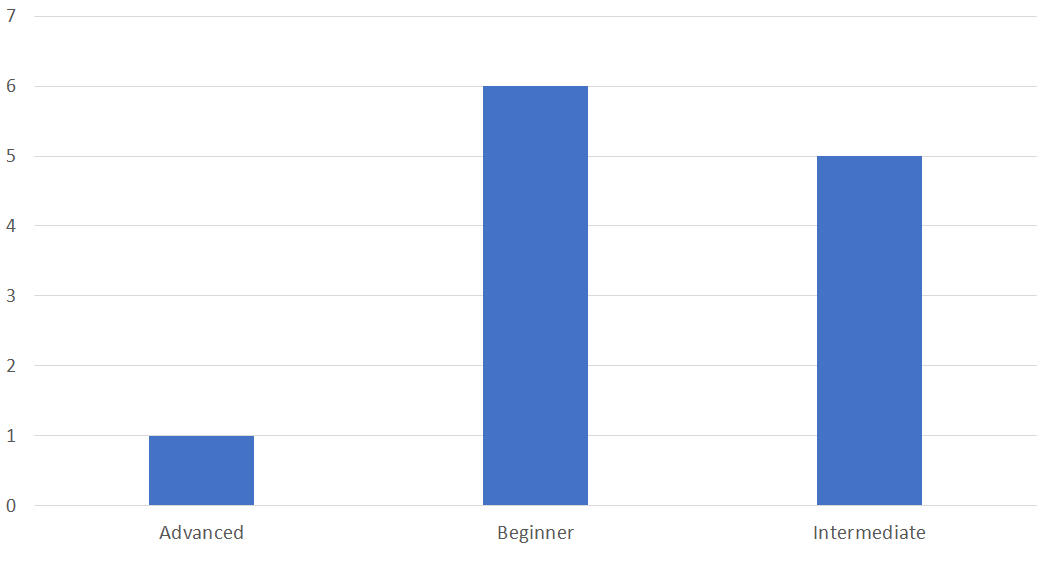
\includegraphics[width=0.9\columnwidth]{prog_knowledge}%
    \caption{\captionstyle{Bar chart showing the overall programming knowledge level of the participants in the survey.}}%
    \label{fig:progknowl}%
\end{figure}


\newpage
\section{Conclusions}

\newpage
\section{Future Work}

\newpage
\bibliographystyle{apalike}
\bibliography{./references}

%you can crate this on a extra tex document just like the title or any other part of the document.
\newpage
\begin{appendices}
\crefalias{section}{appsec}
\section{Project Overview}
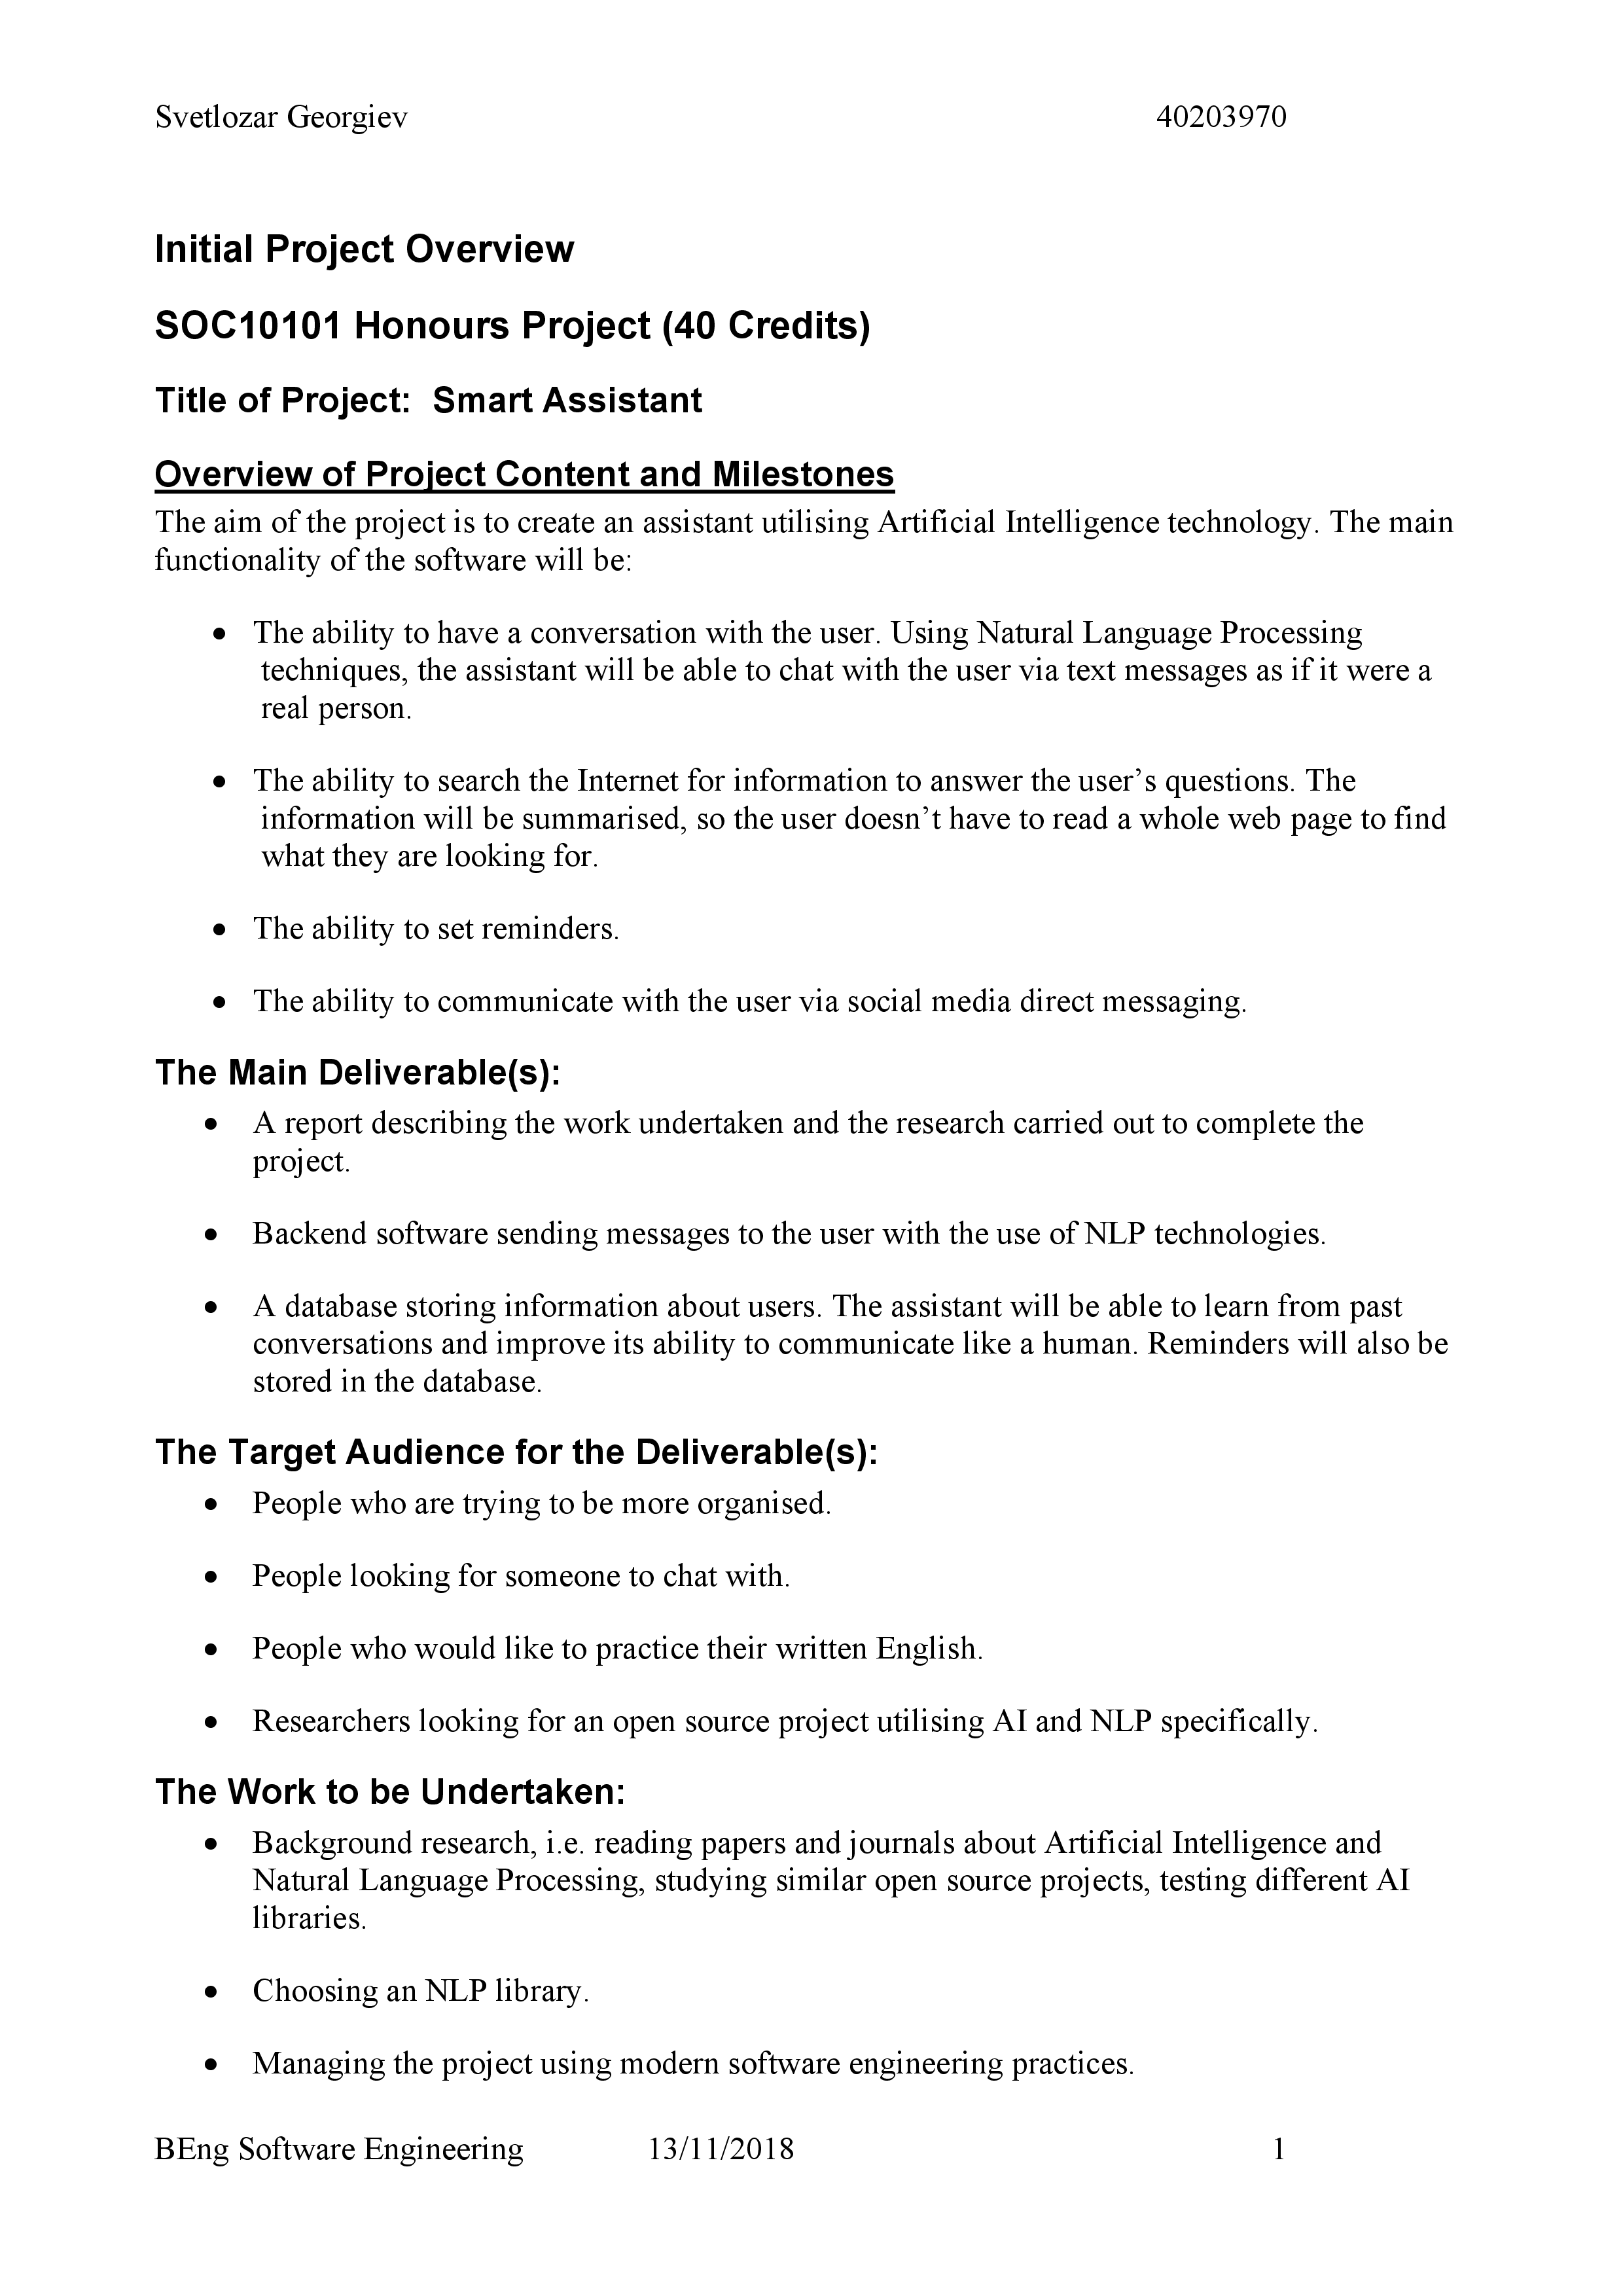
\includegraphics[width=\textwidth,height=\textheight,keepaspectratio]{IPO-0.png} % fit images to page
\newpage
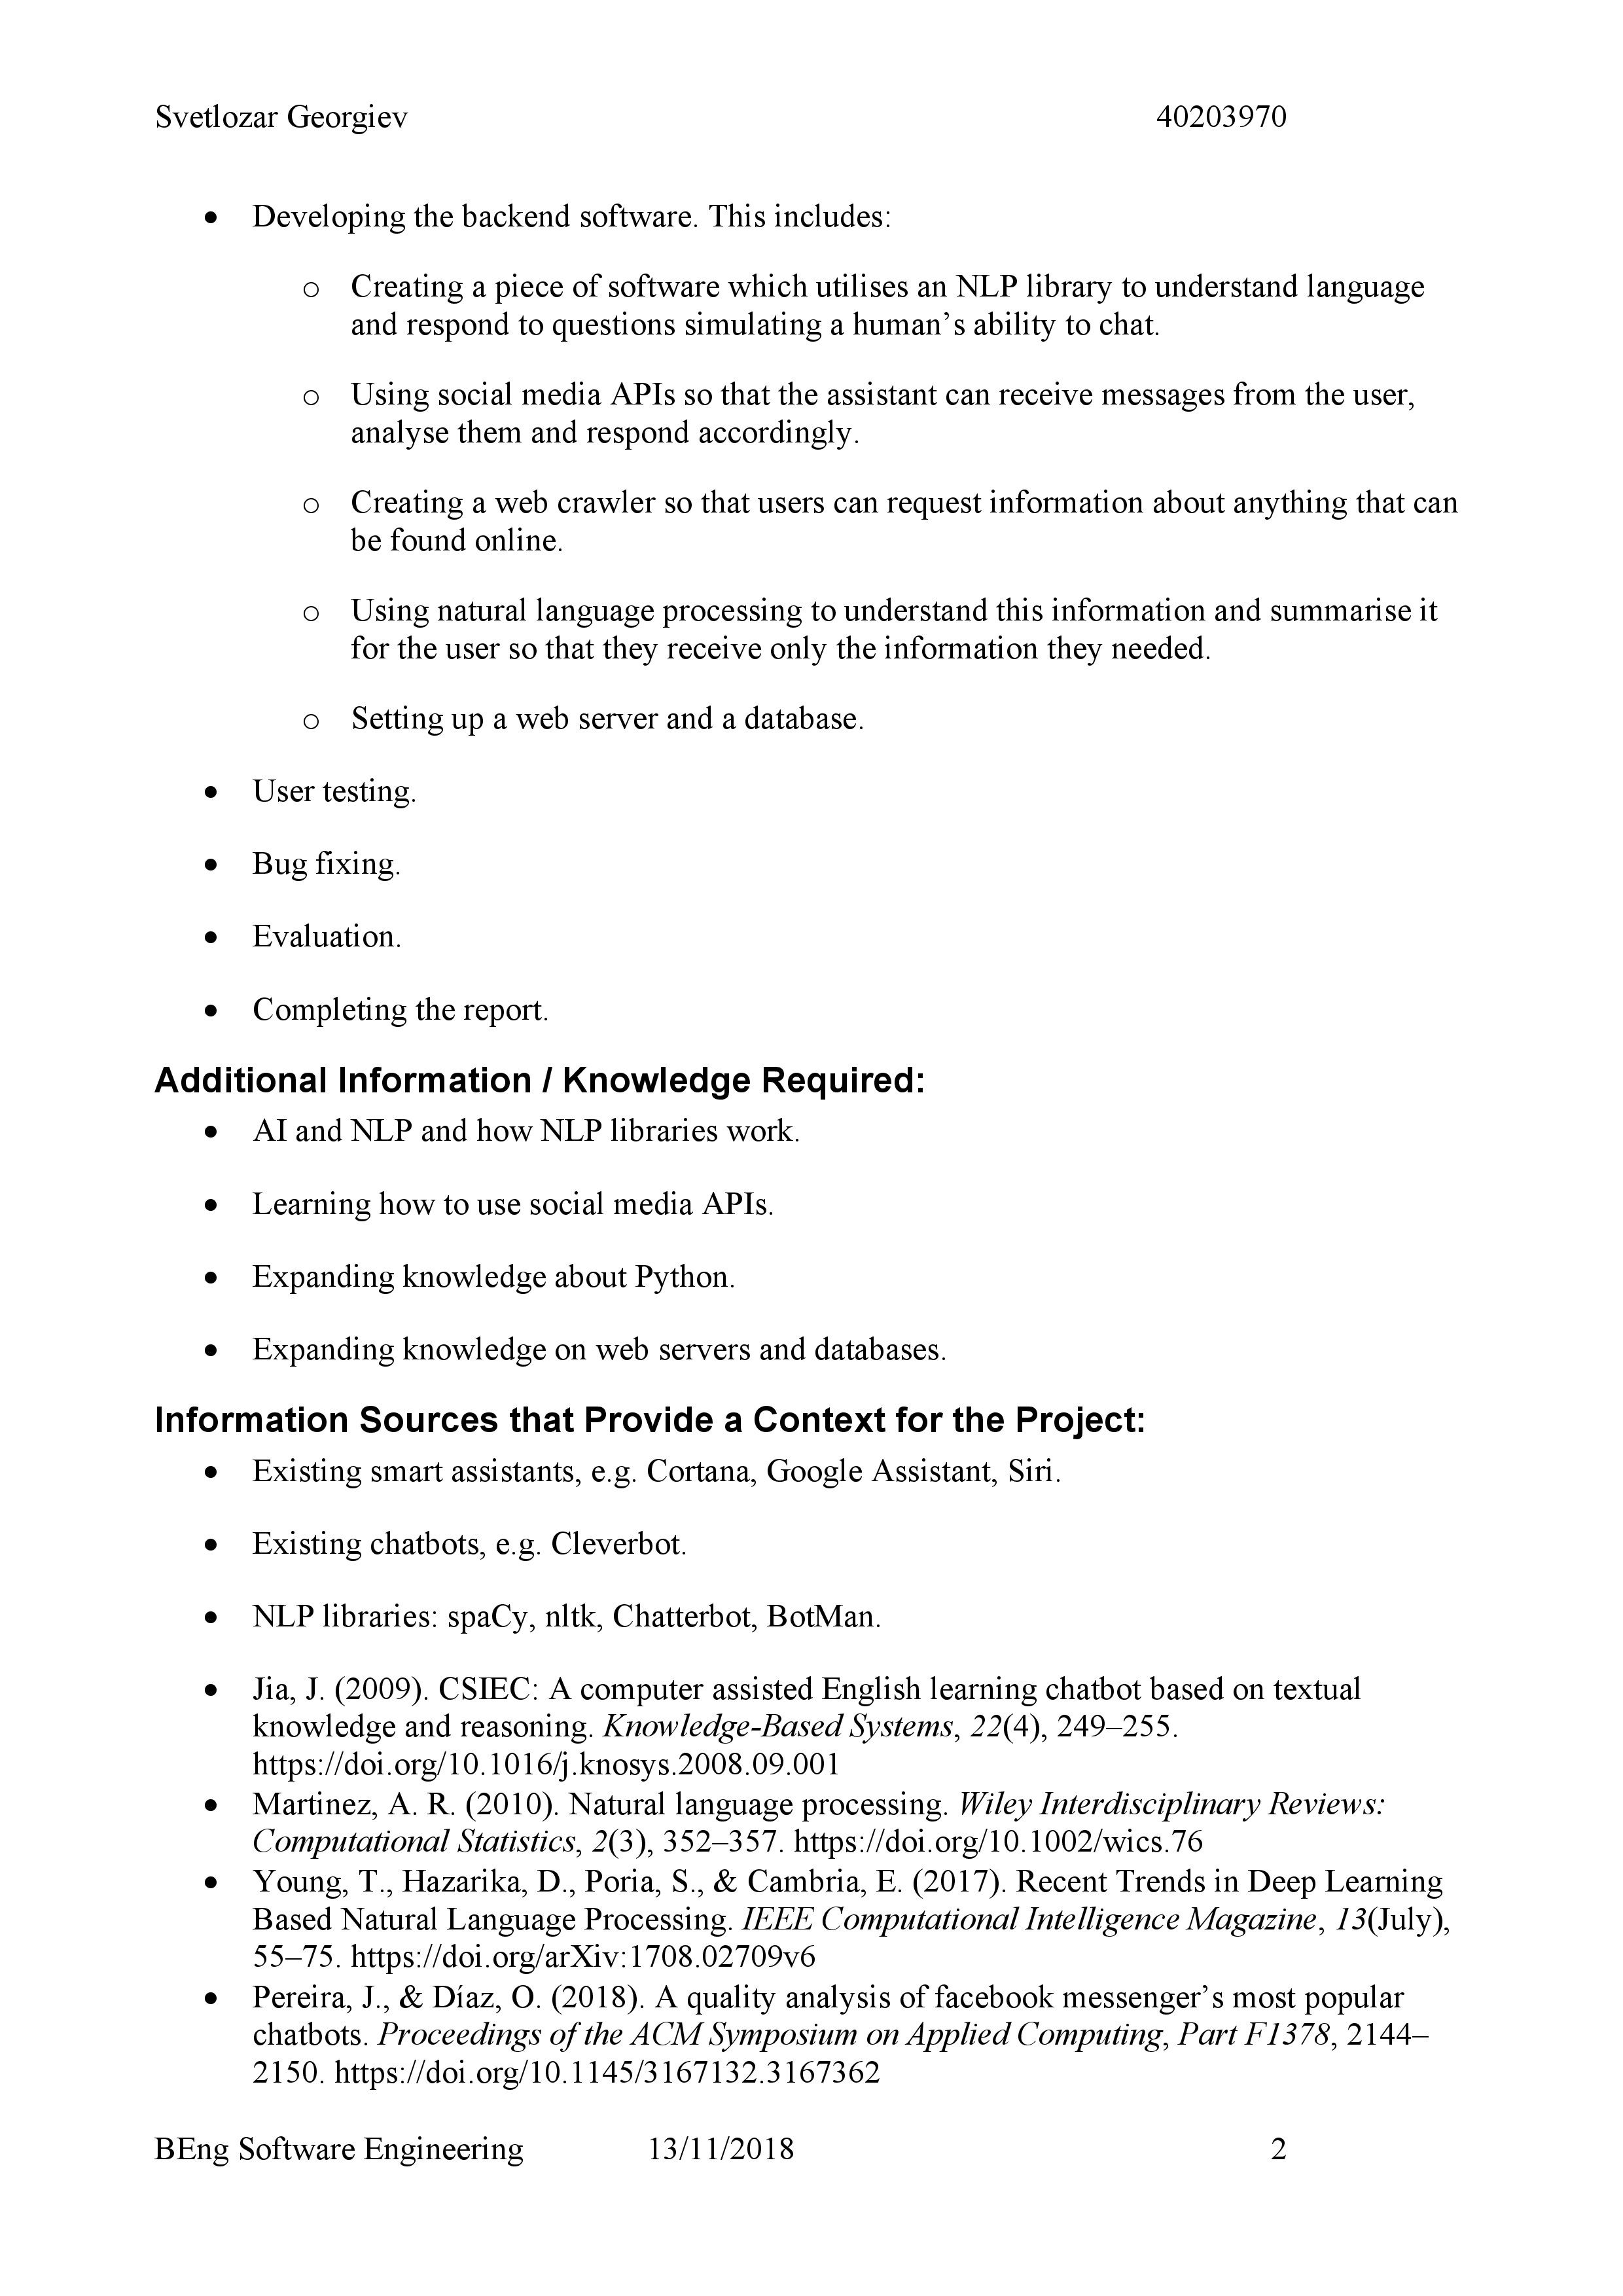
\includegraphics[width=\textwidth,height=\textheight,keepaspectratio]{IPO-1.png}
\newpage
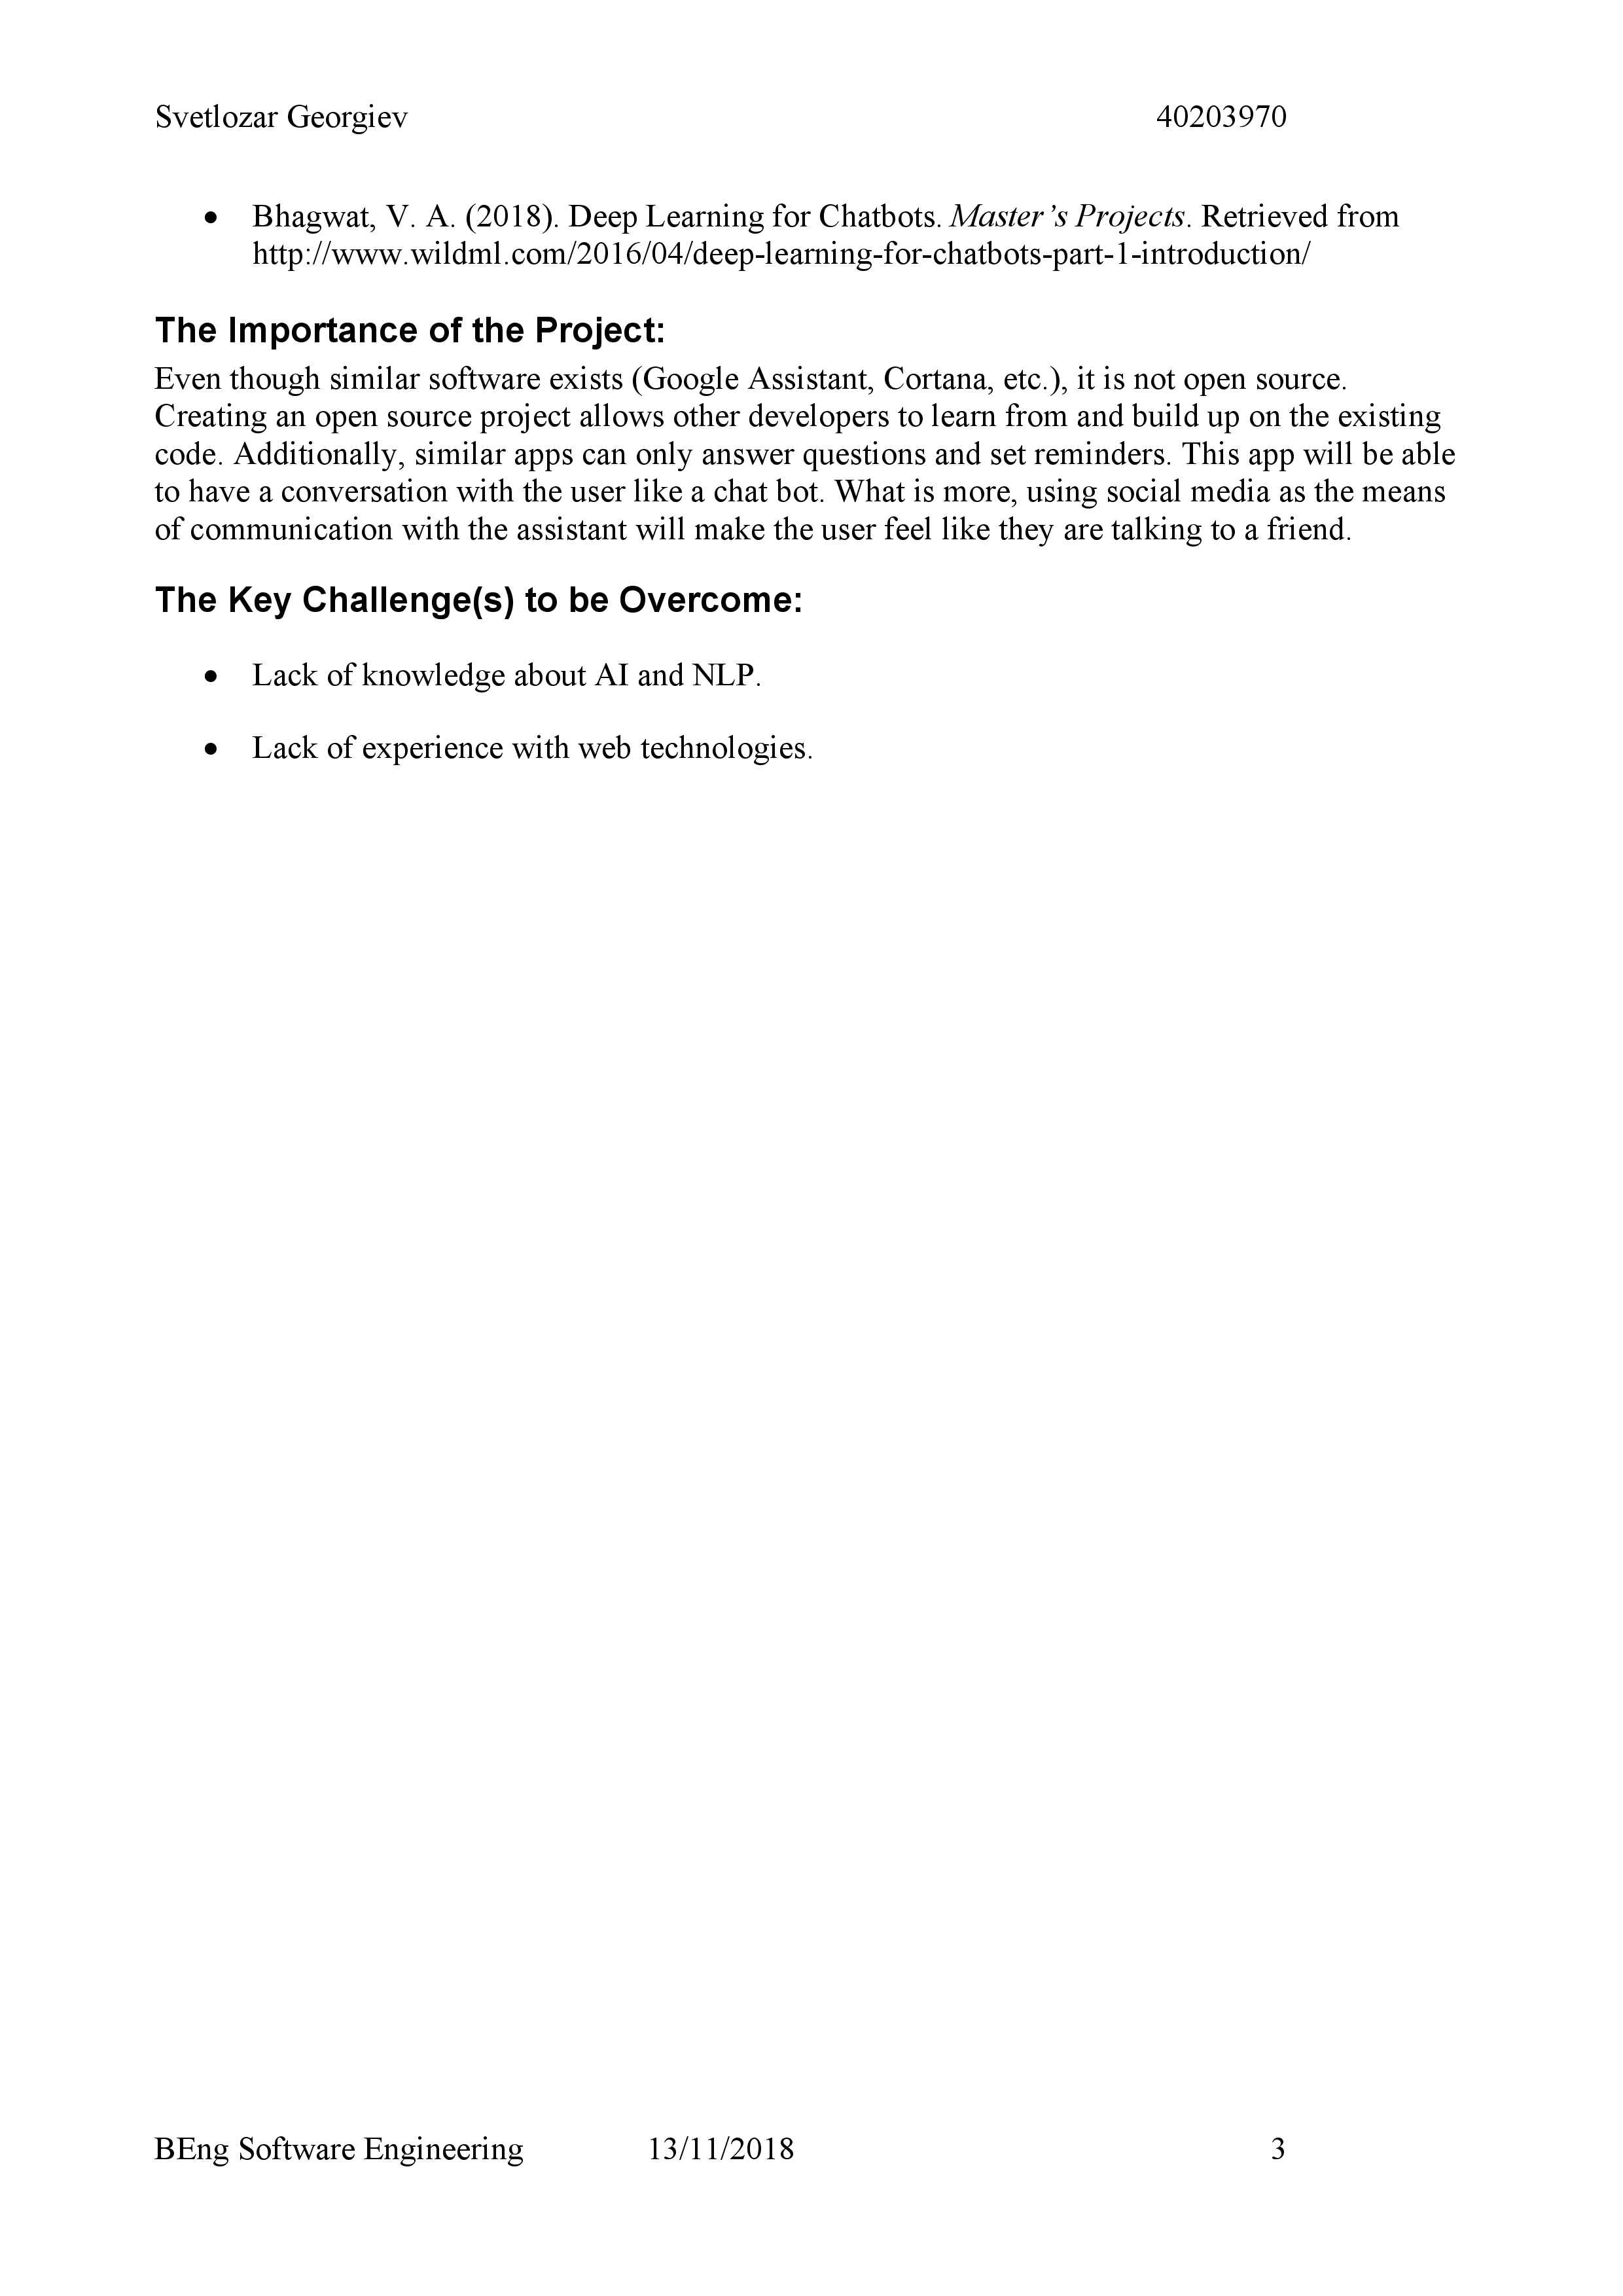
\includegraphics[width=\textwidth,height=\textheight,keepaspectratio]{IPO-2.png}

\newpage
\section{Diary Sheets}
% first semester
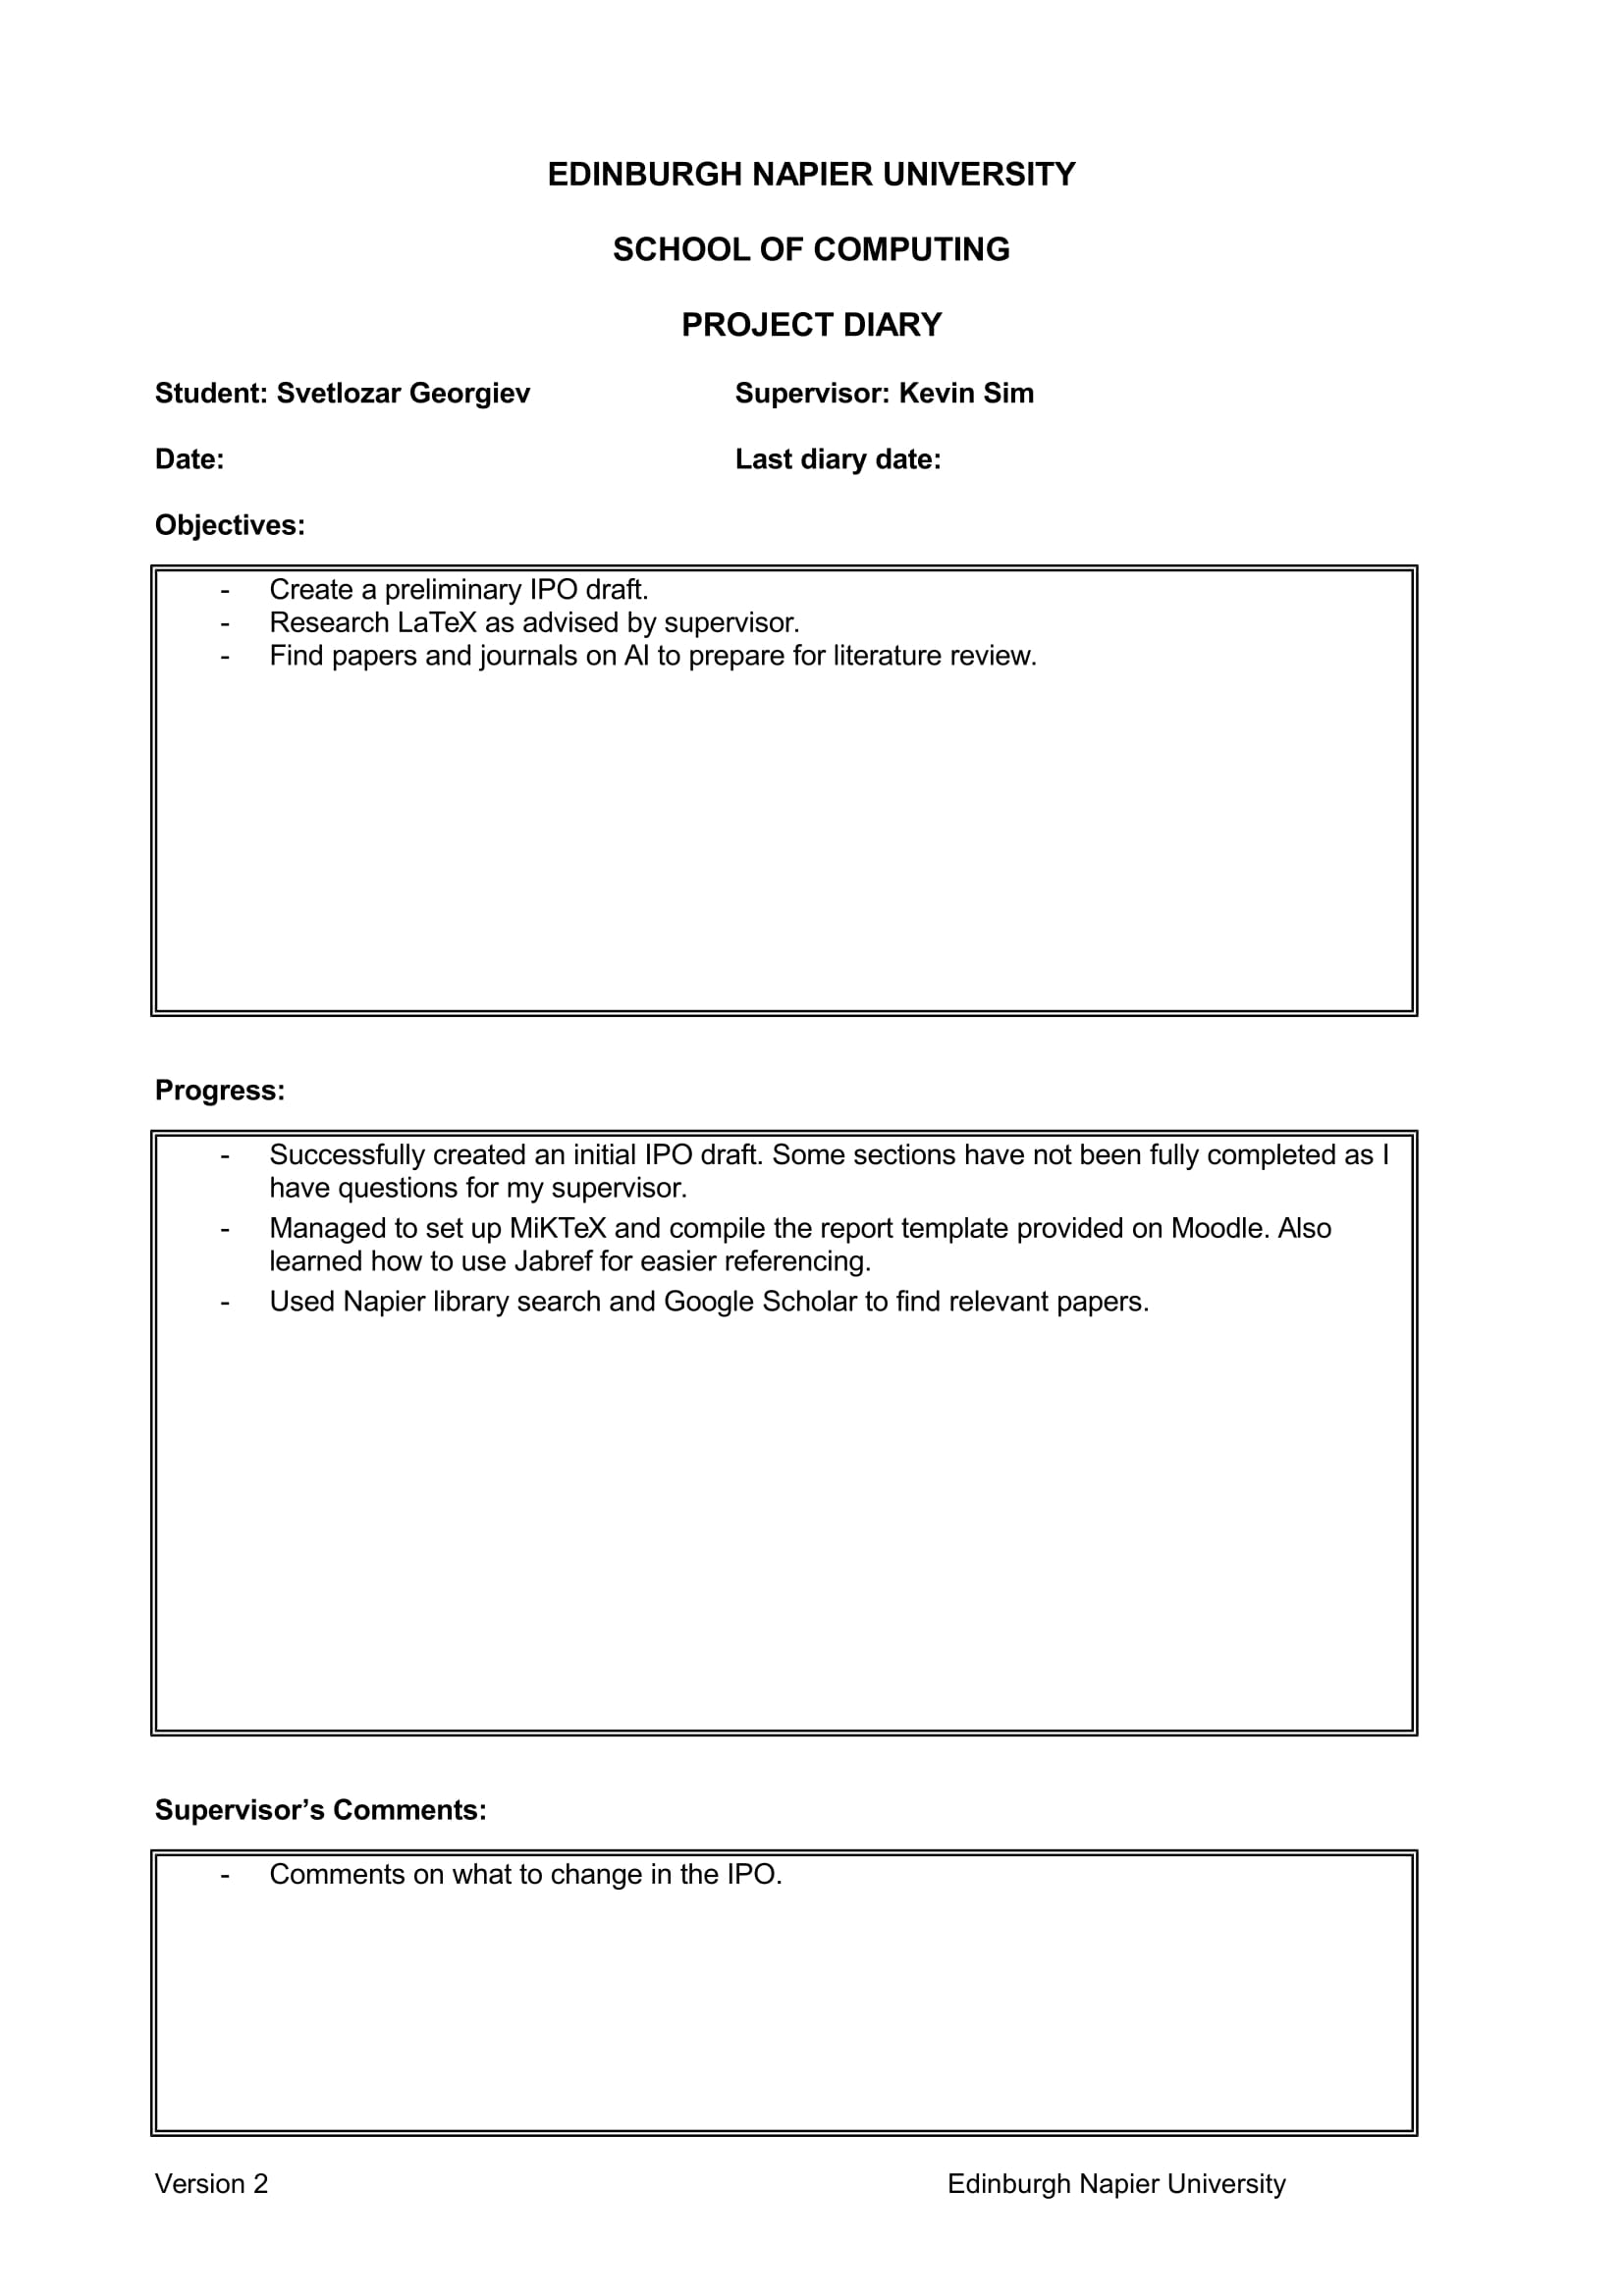
\includegraphics[width=\textwidth,height=\textheight,keepaspectratio]{week2.jpg} % fit images to page
\newpage
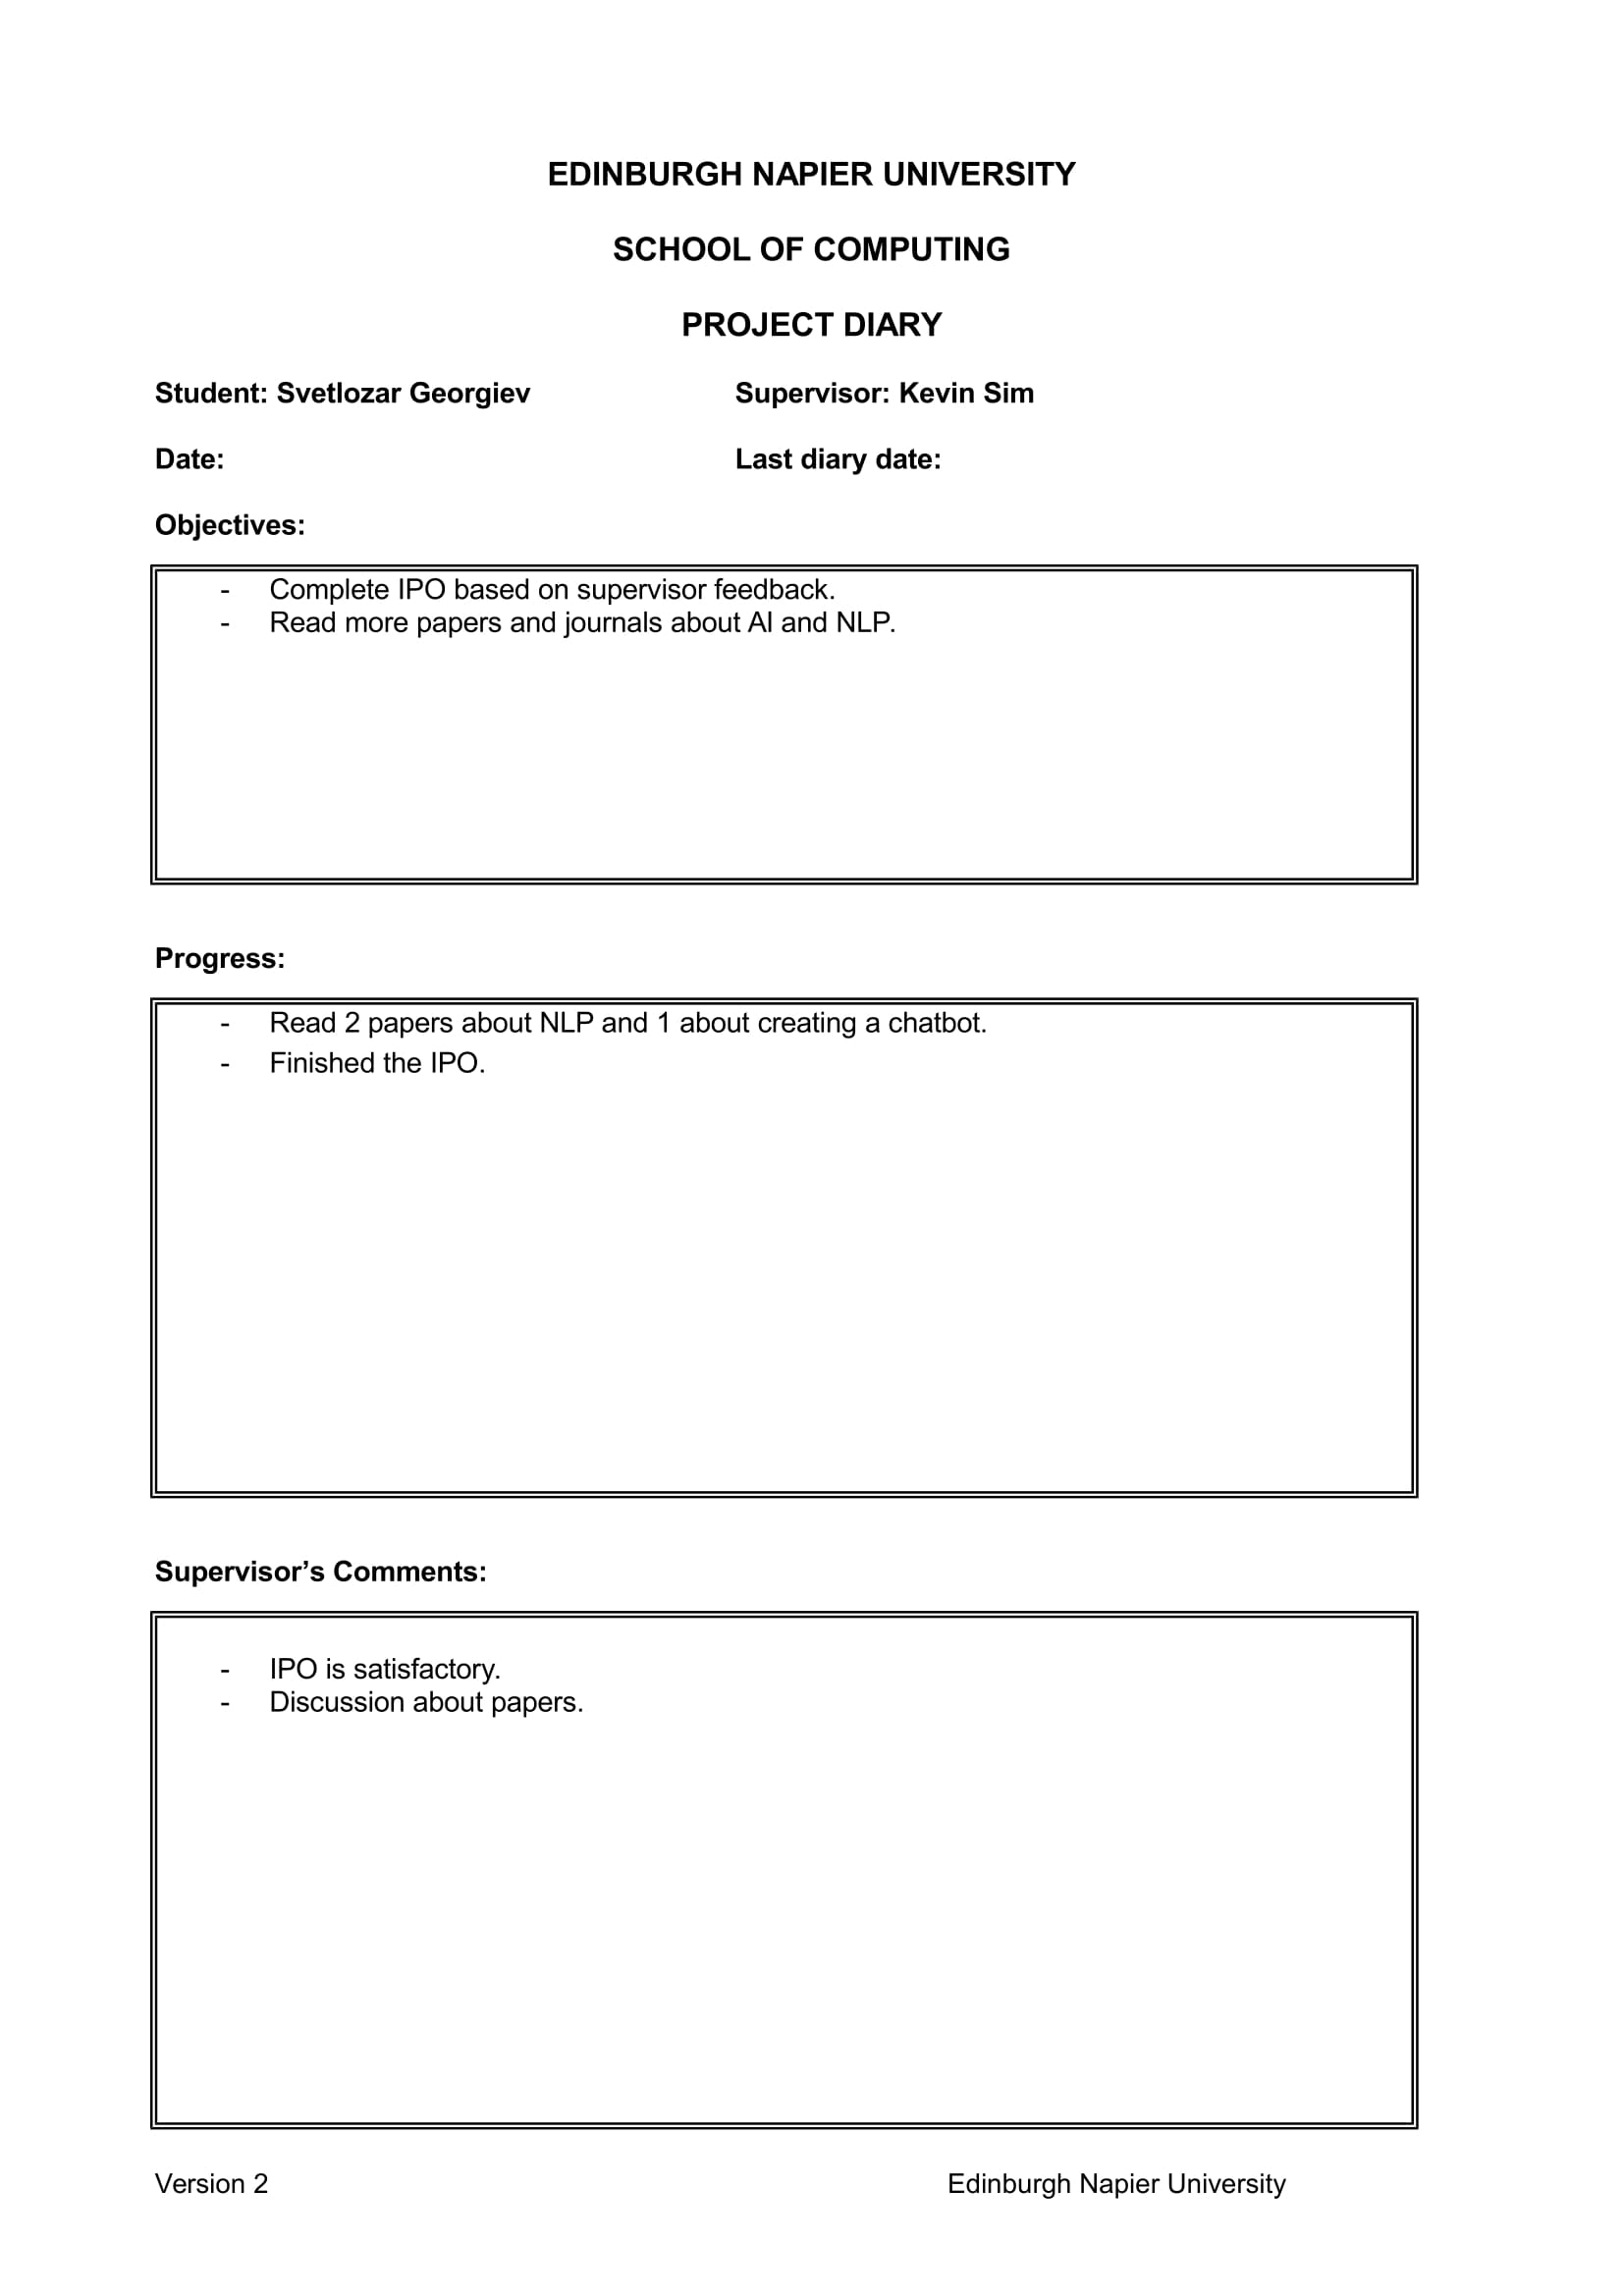
\includegraphics[width=\textwidth,height=\textheight,keepaspectratio]{week3.jpg}
\newpage
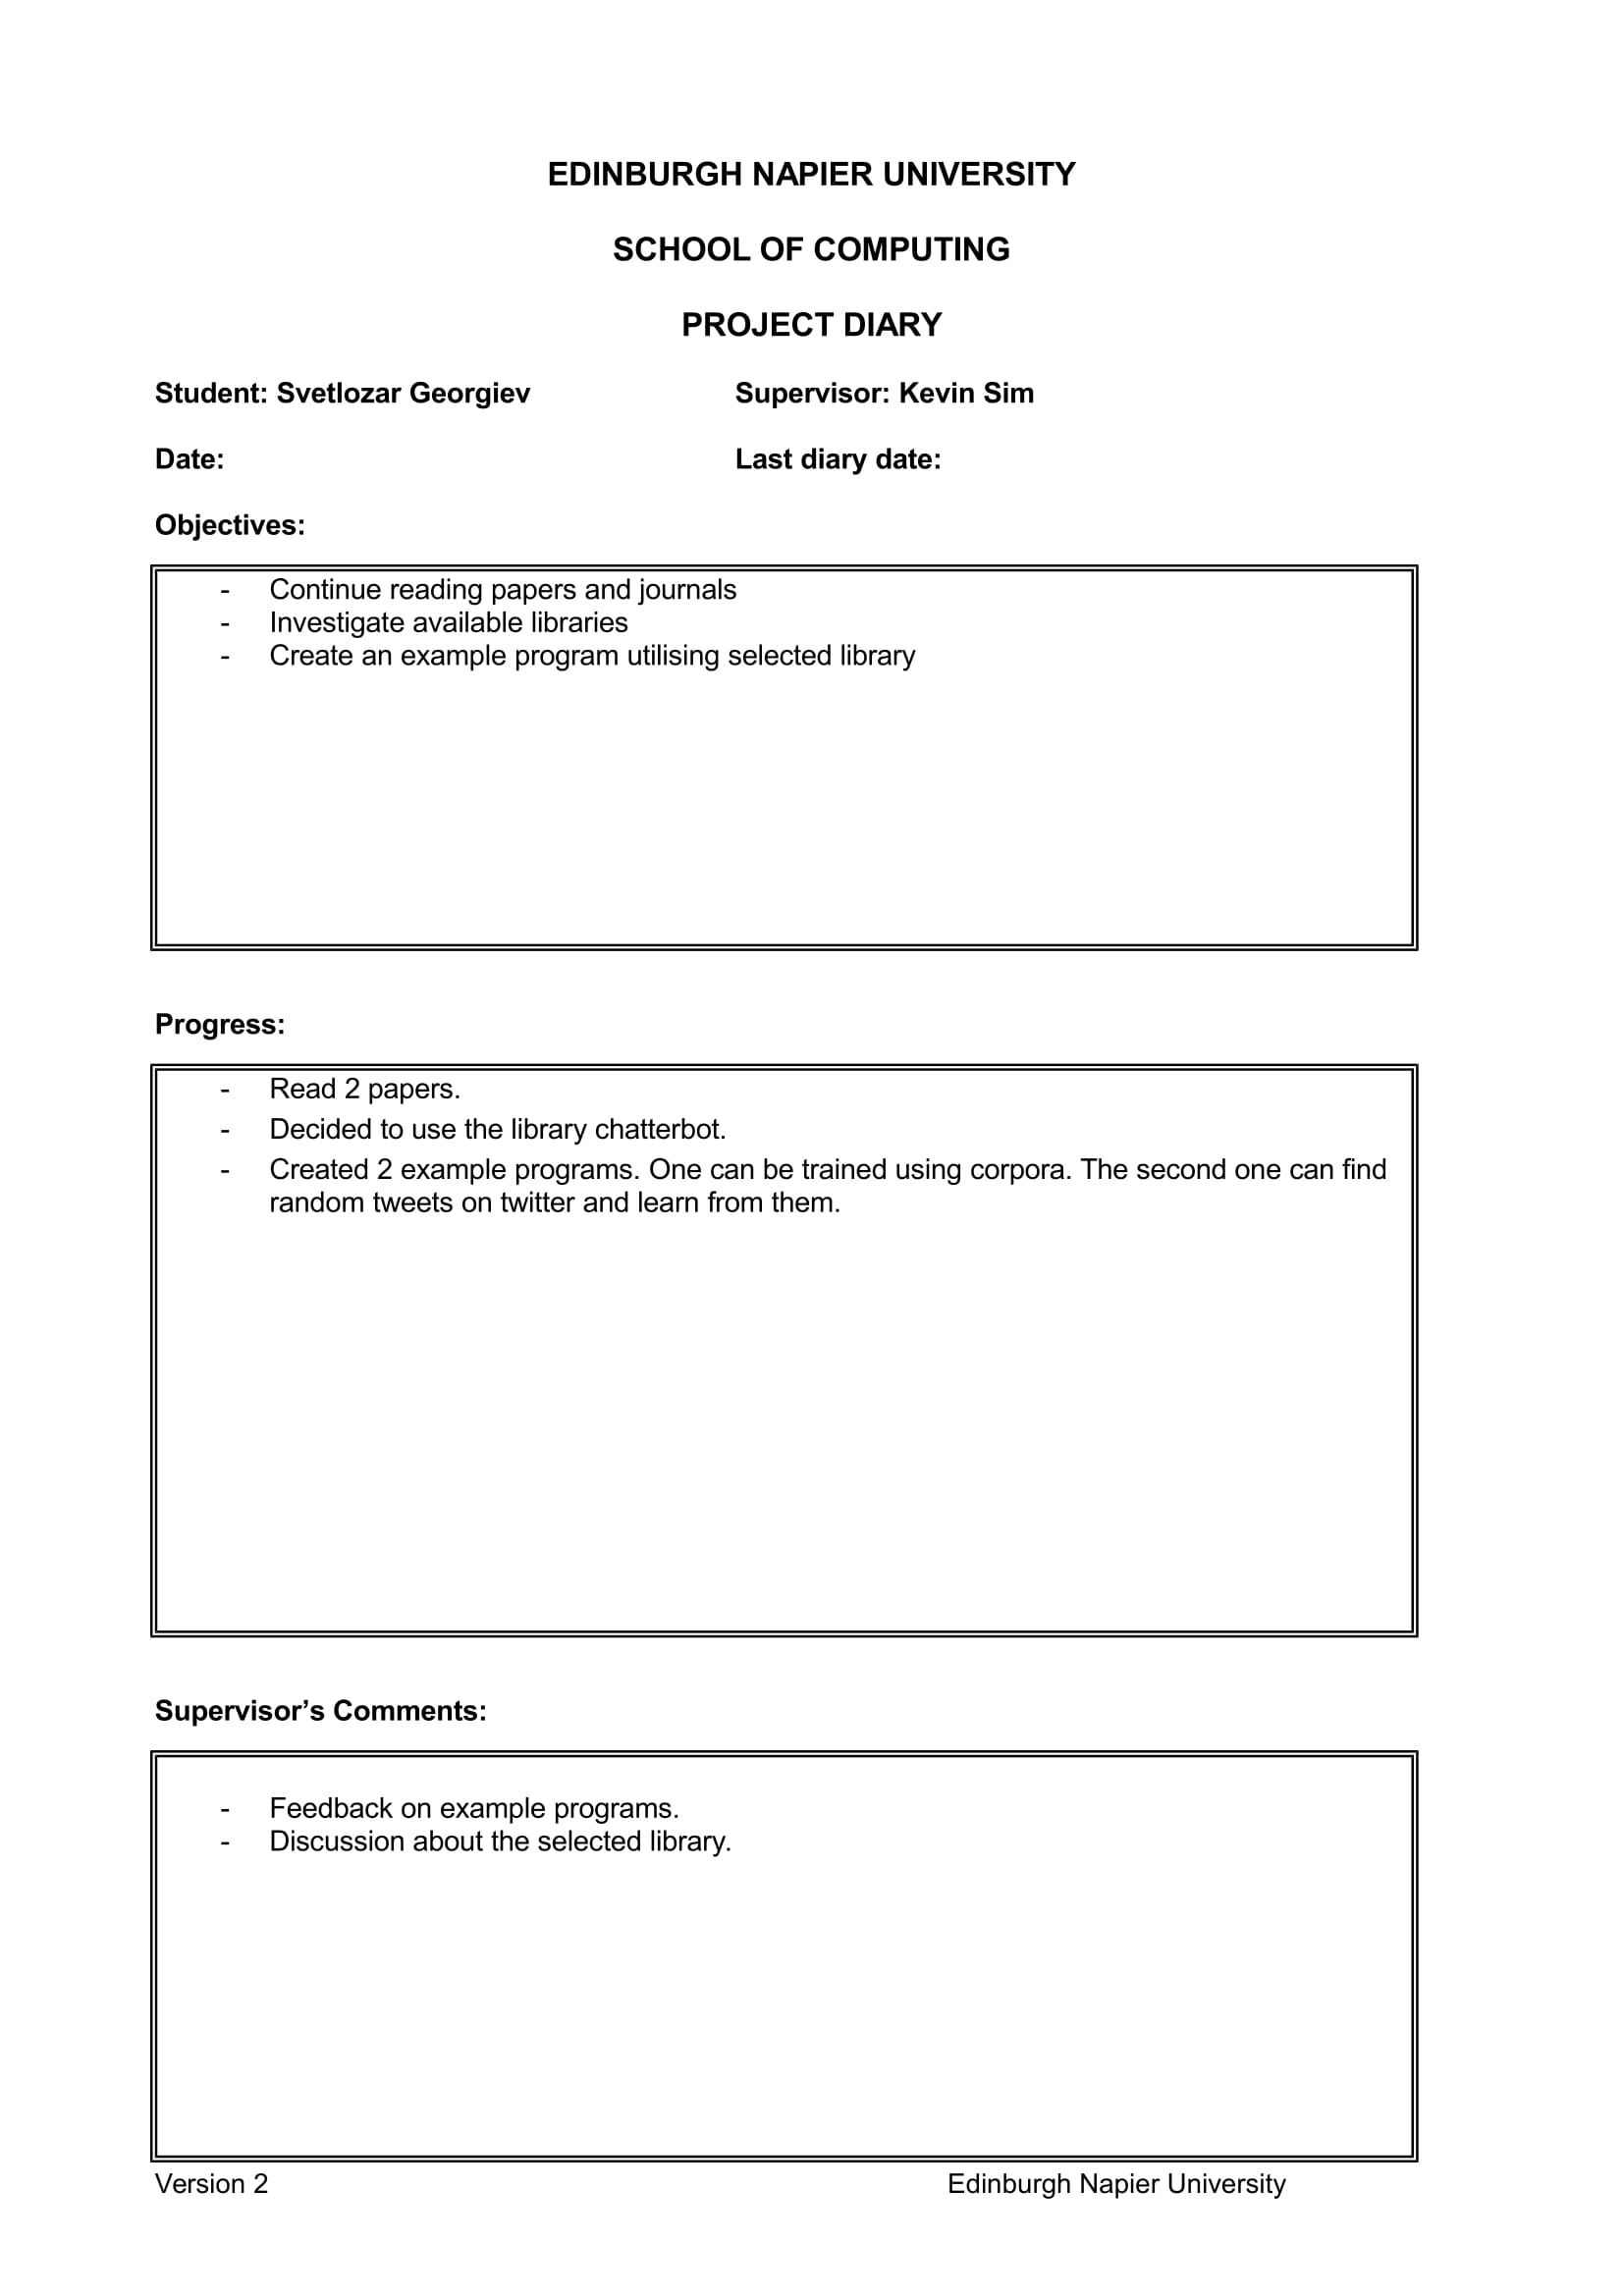
\includegraphics[width=\textwidth,height=\textheight,keepaspectratio]{week4.jpg}
\newpage
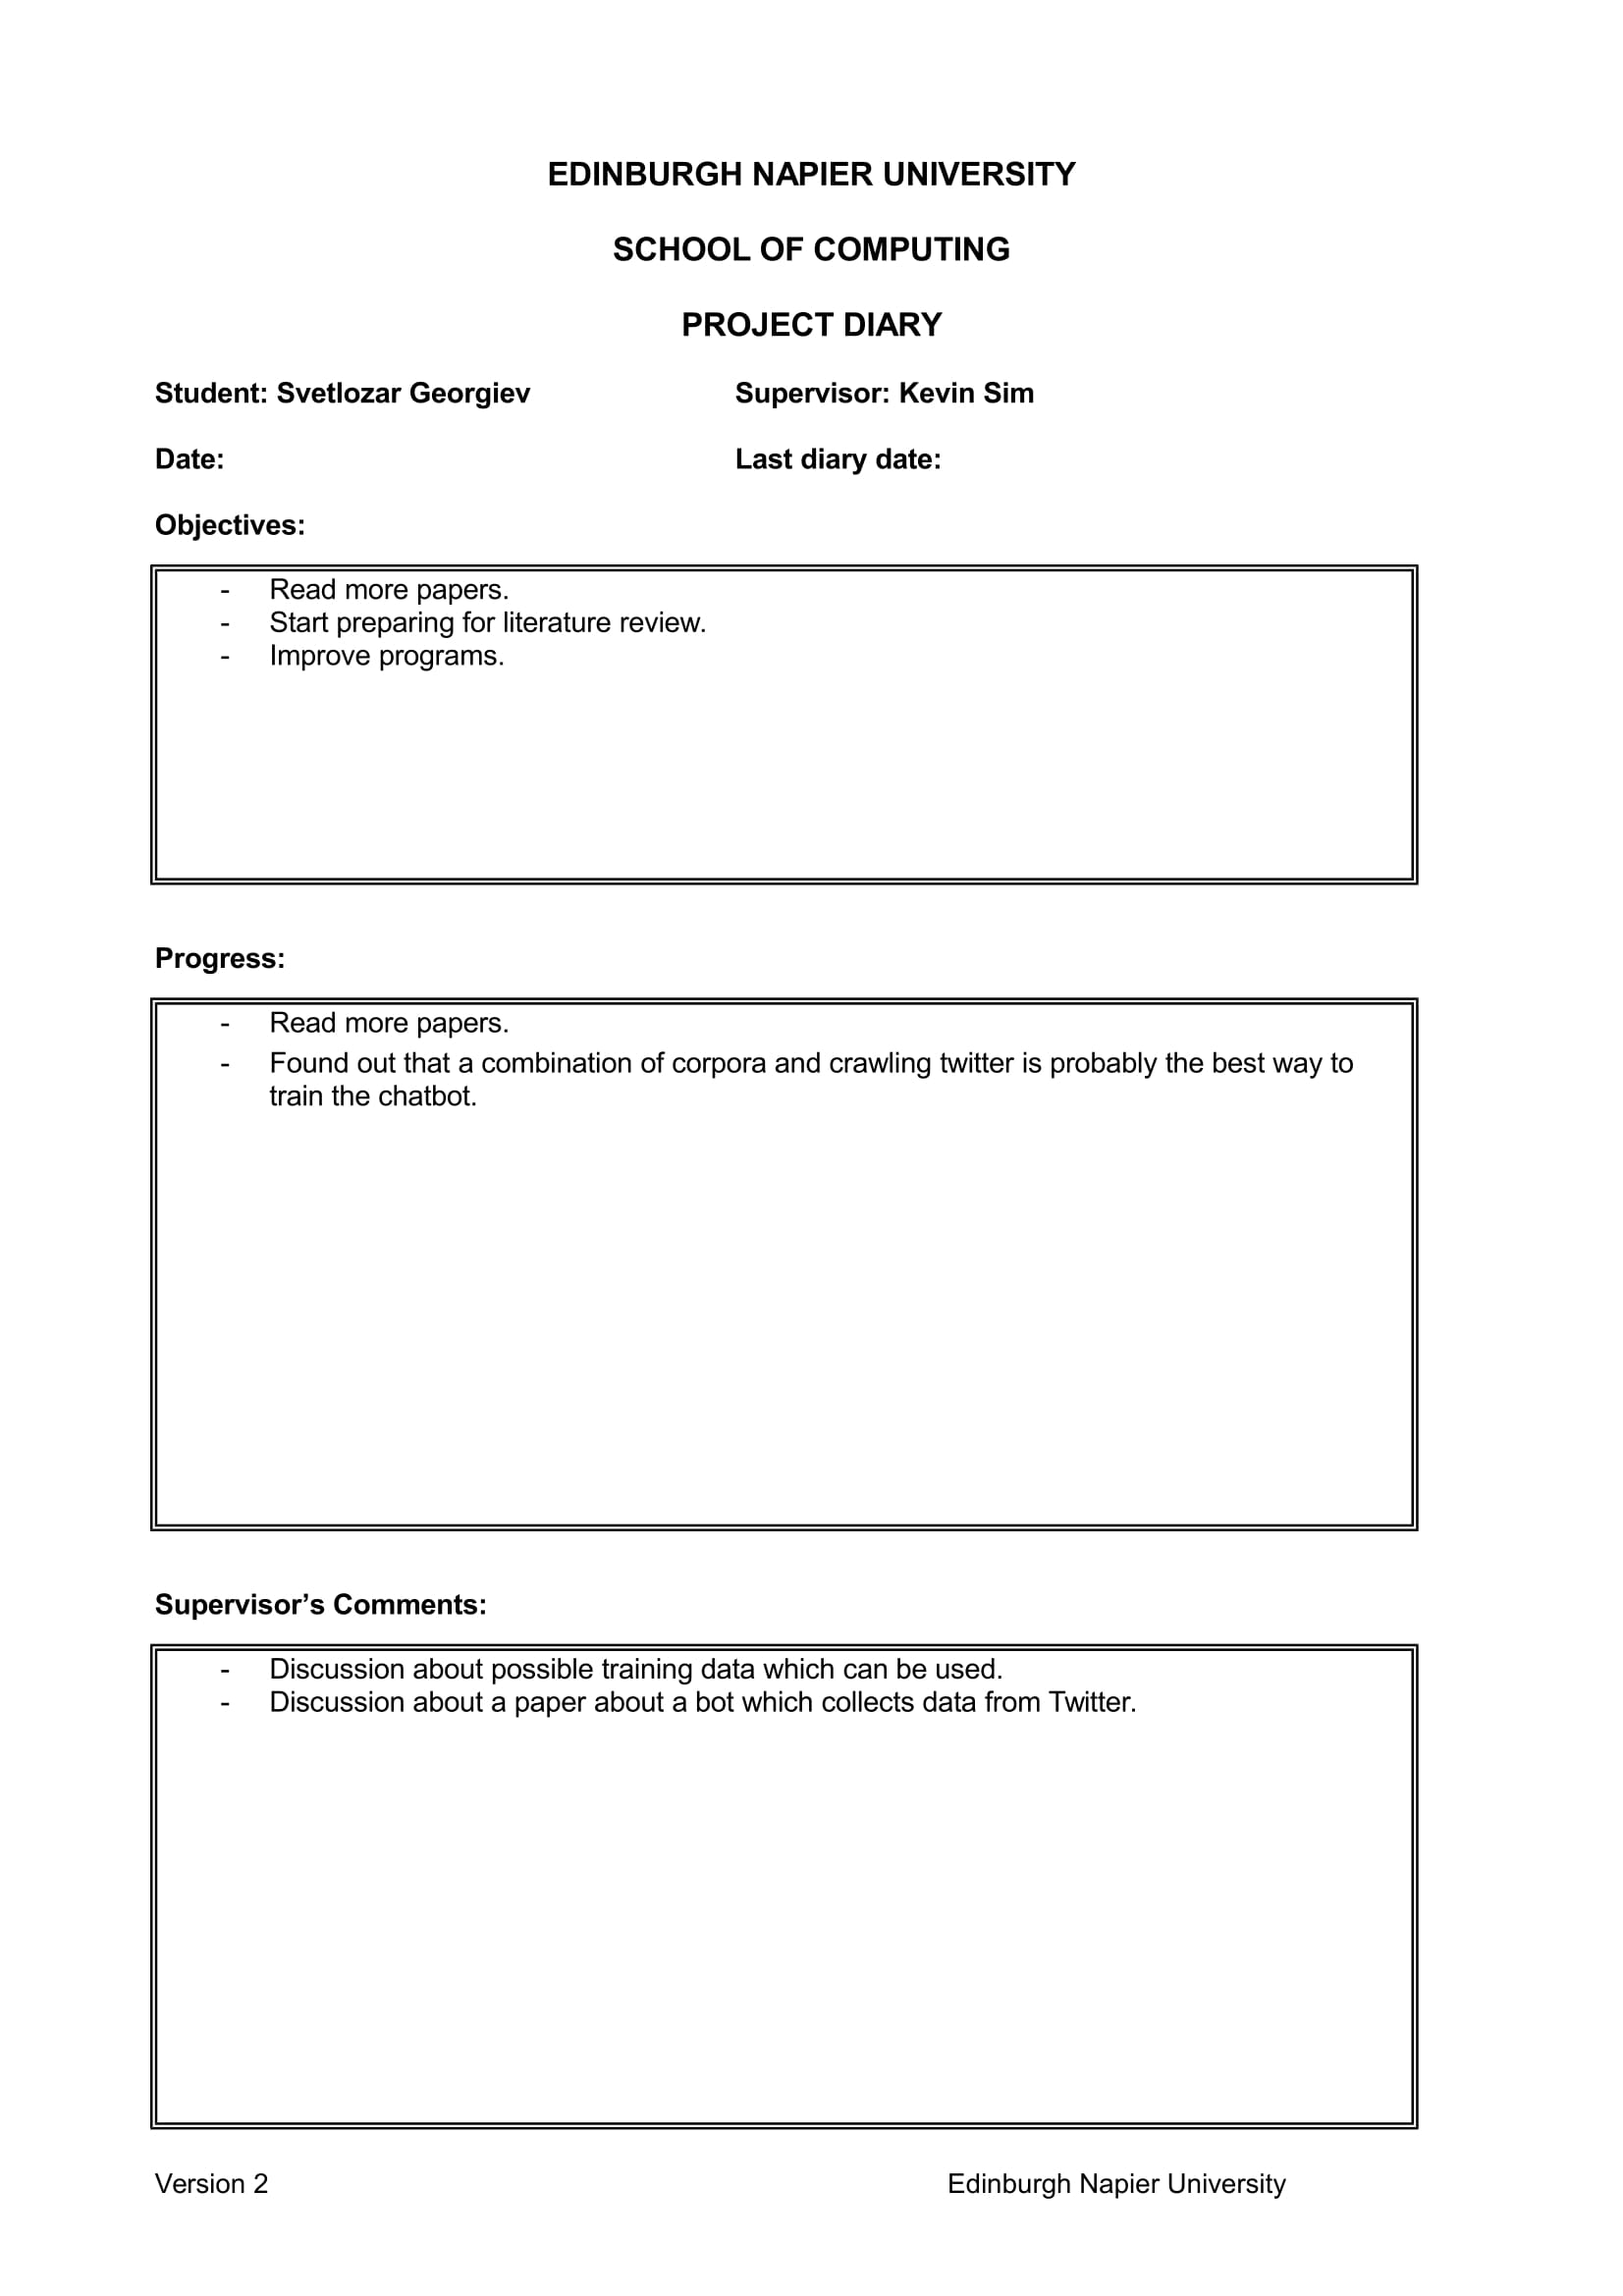
\includegraphics[width=\textwidth,height=\textheight,keepaspectratio]{week5.jpg}
\newpage
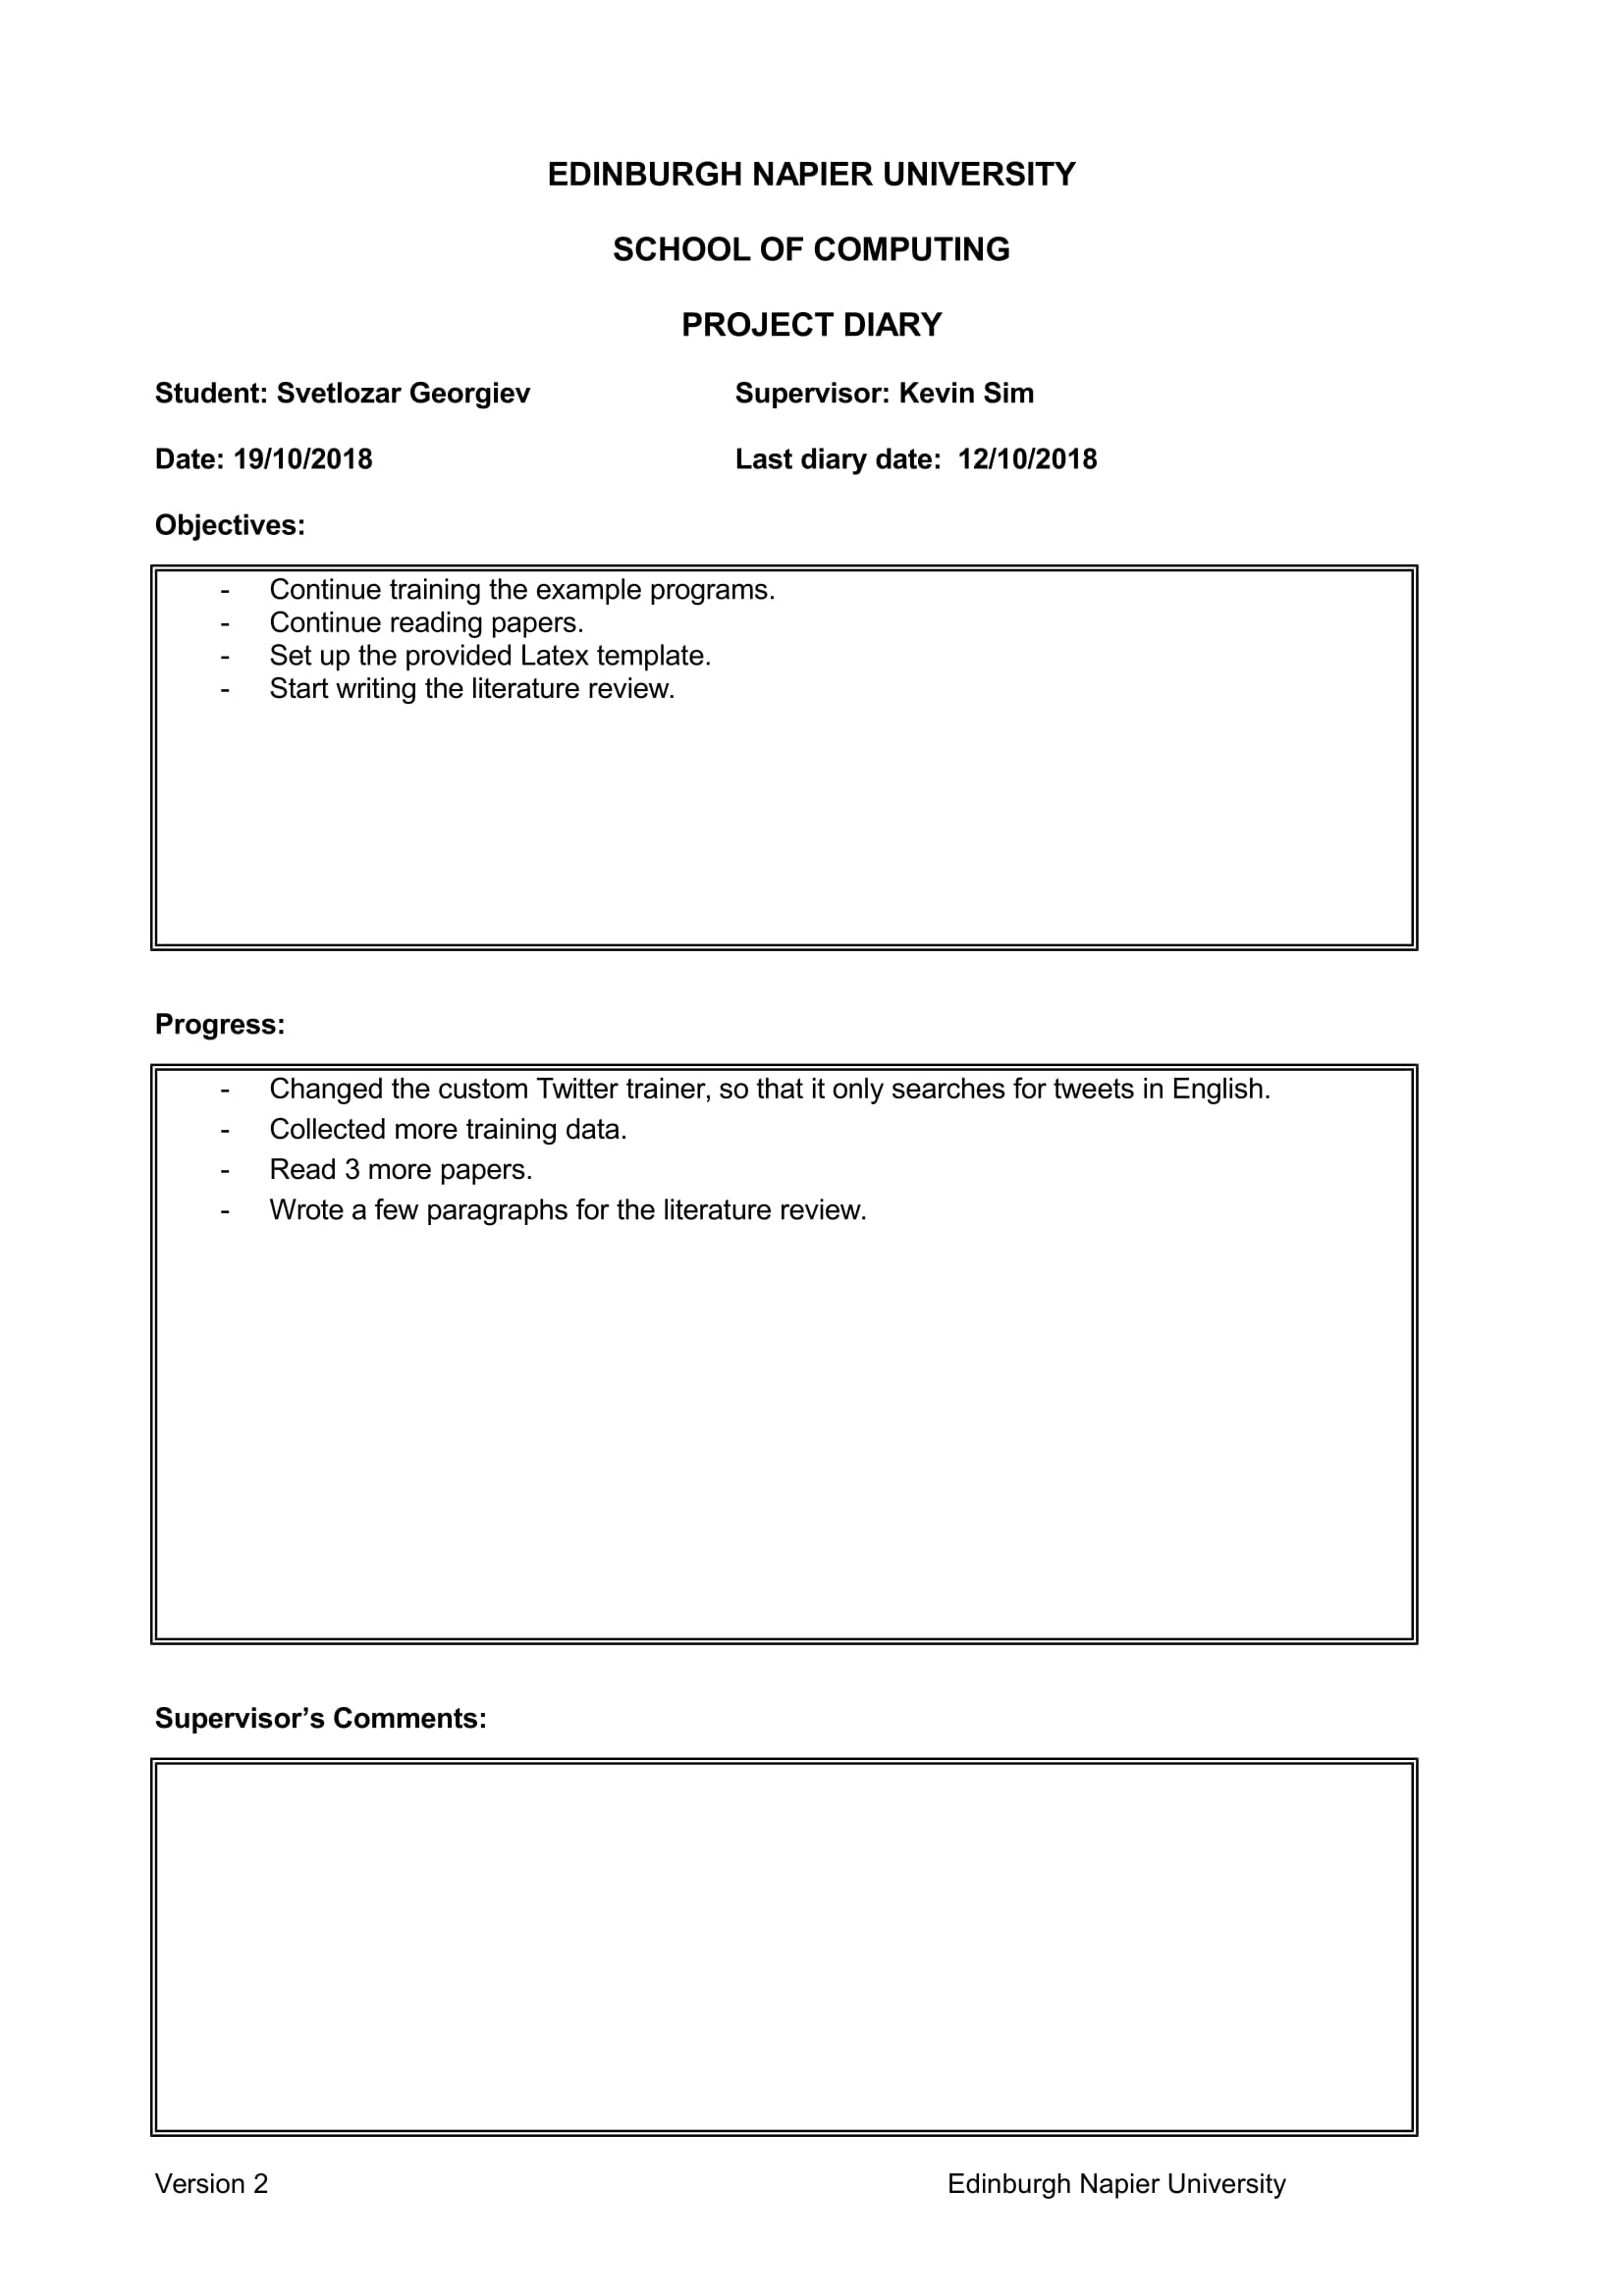
\includegraphics[width=\textwidth,height=\textheight,keepaspectratio]{week6.jpg}
\newpage
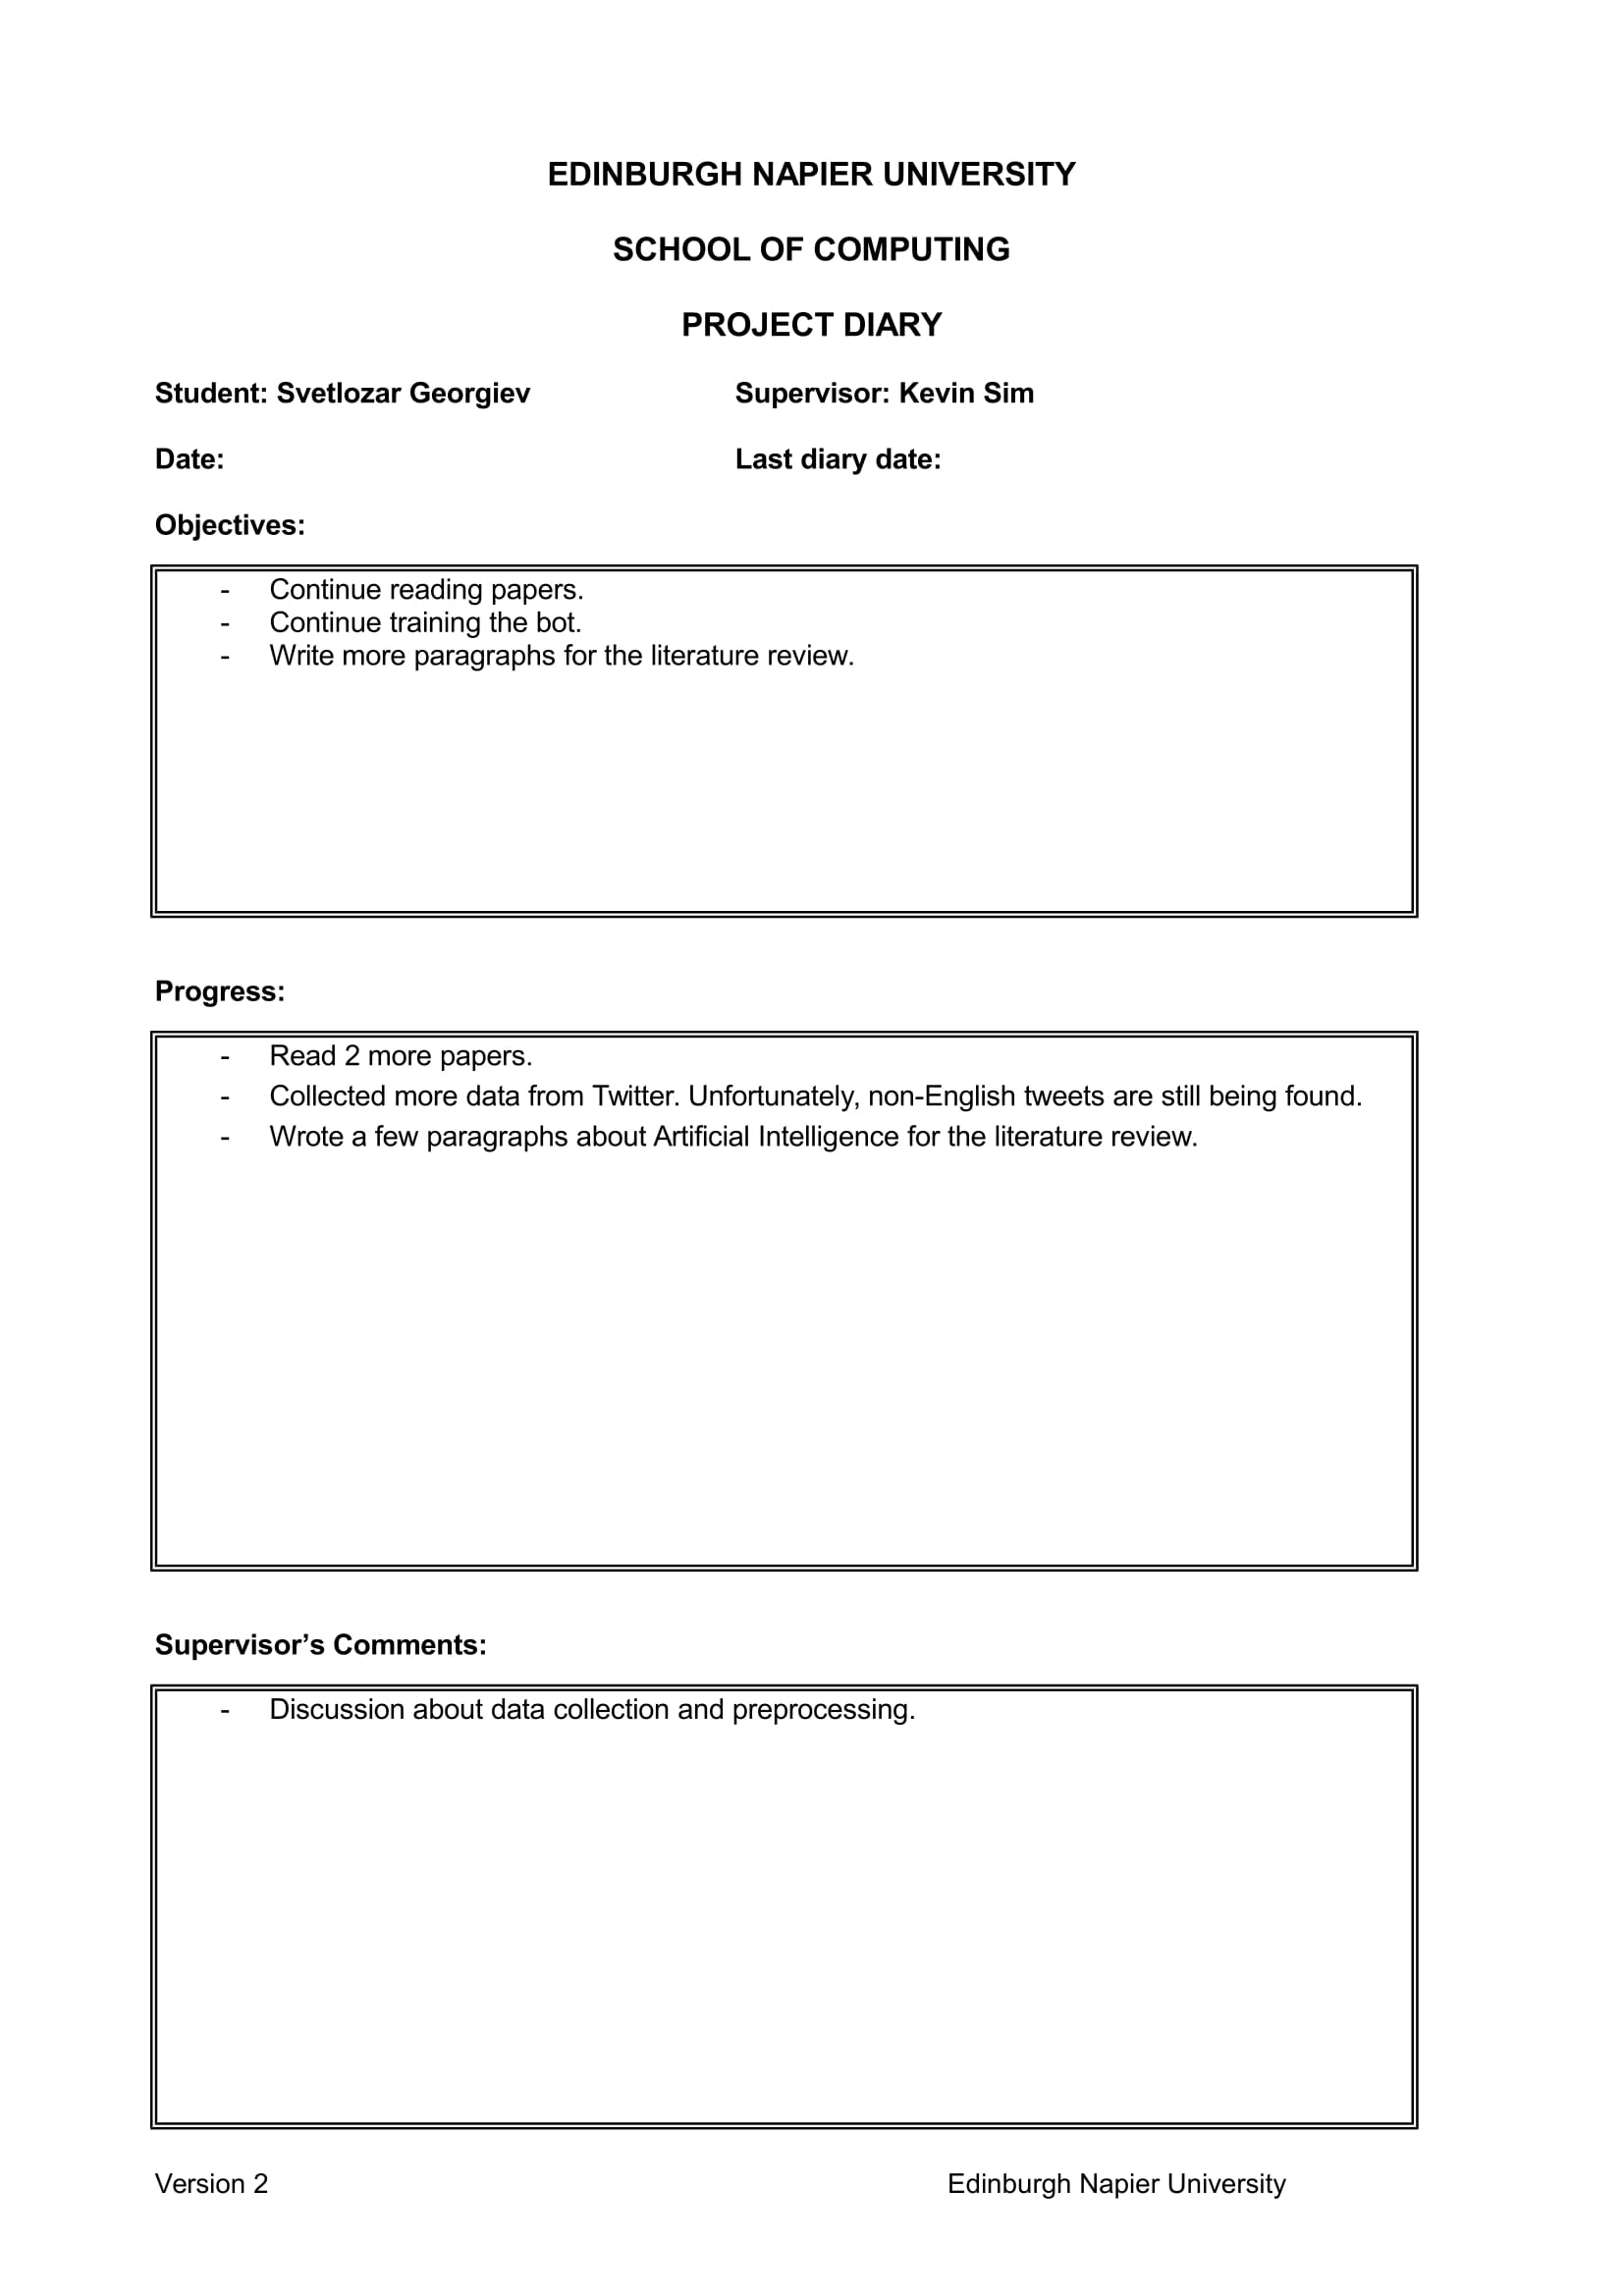
\includegraphics[width=\textwidth,height=\textheight,keepaspectratio]{week7.jpg}
\newpage
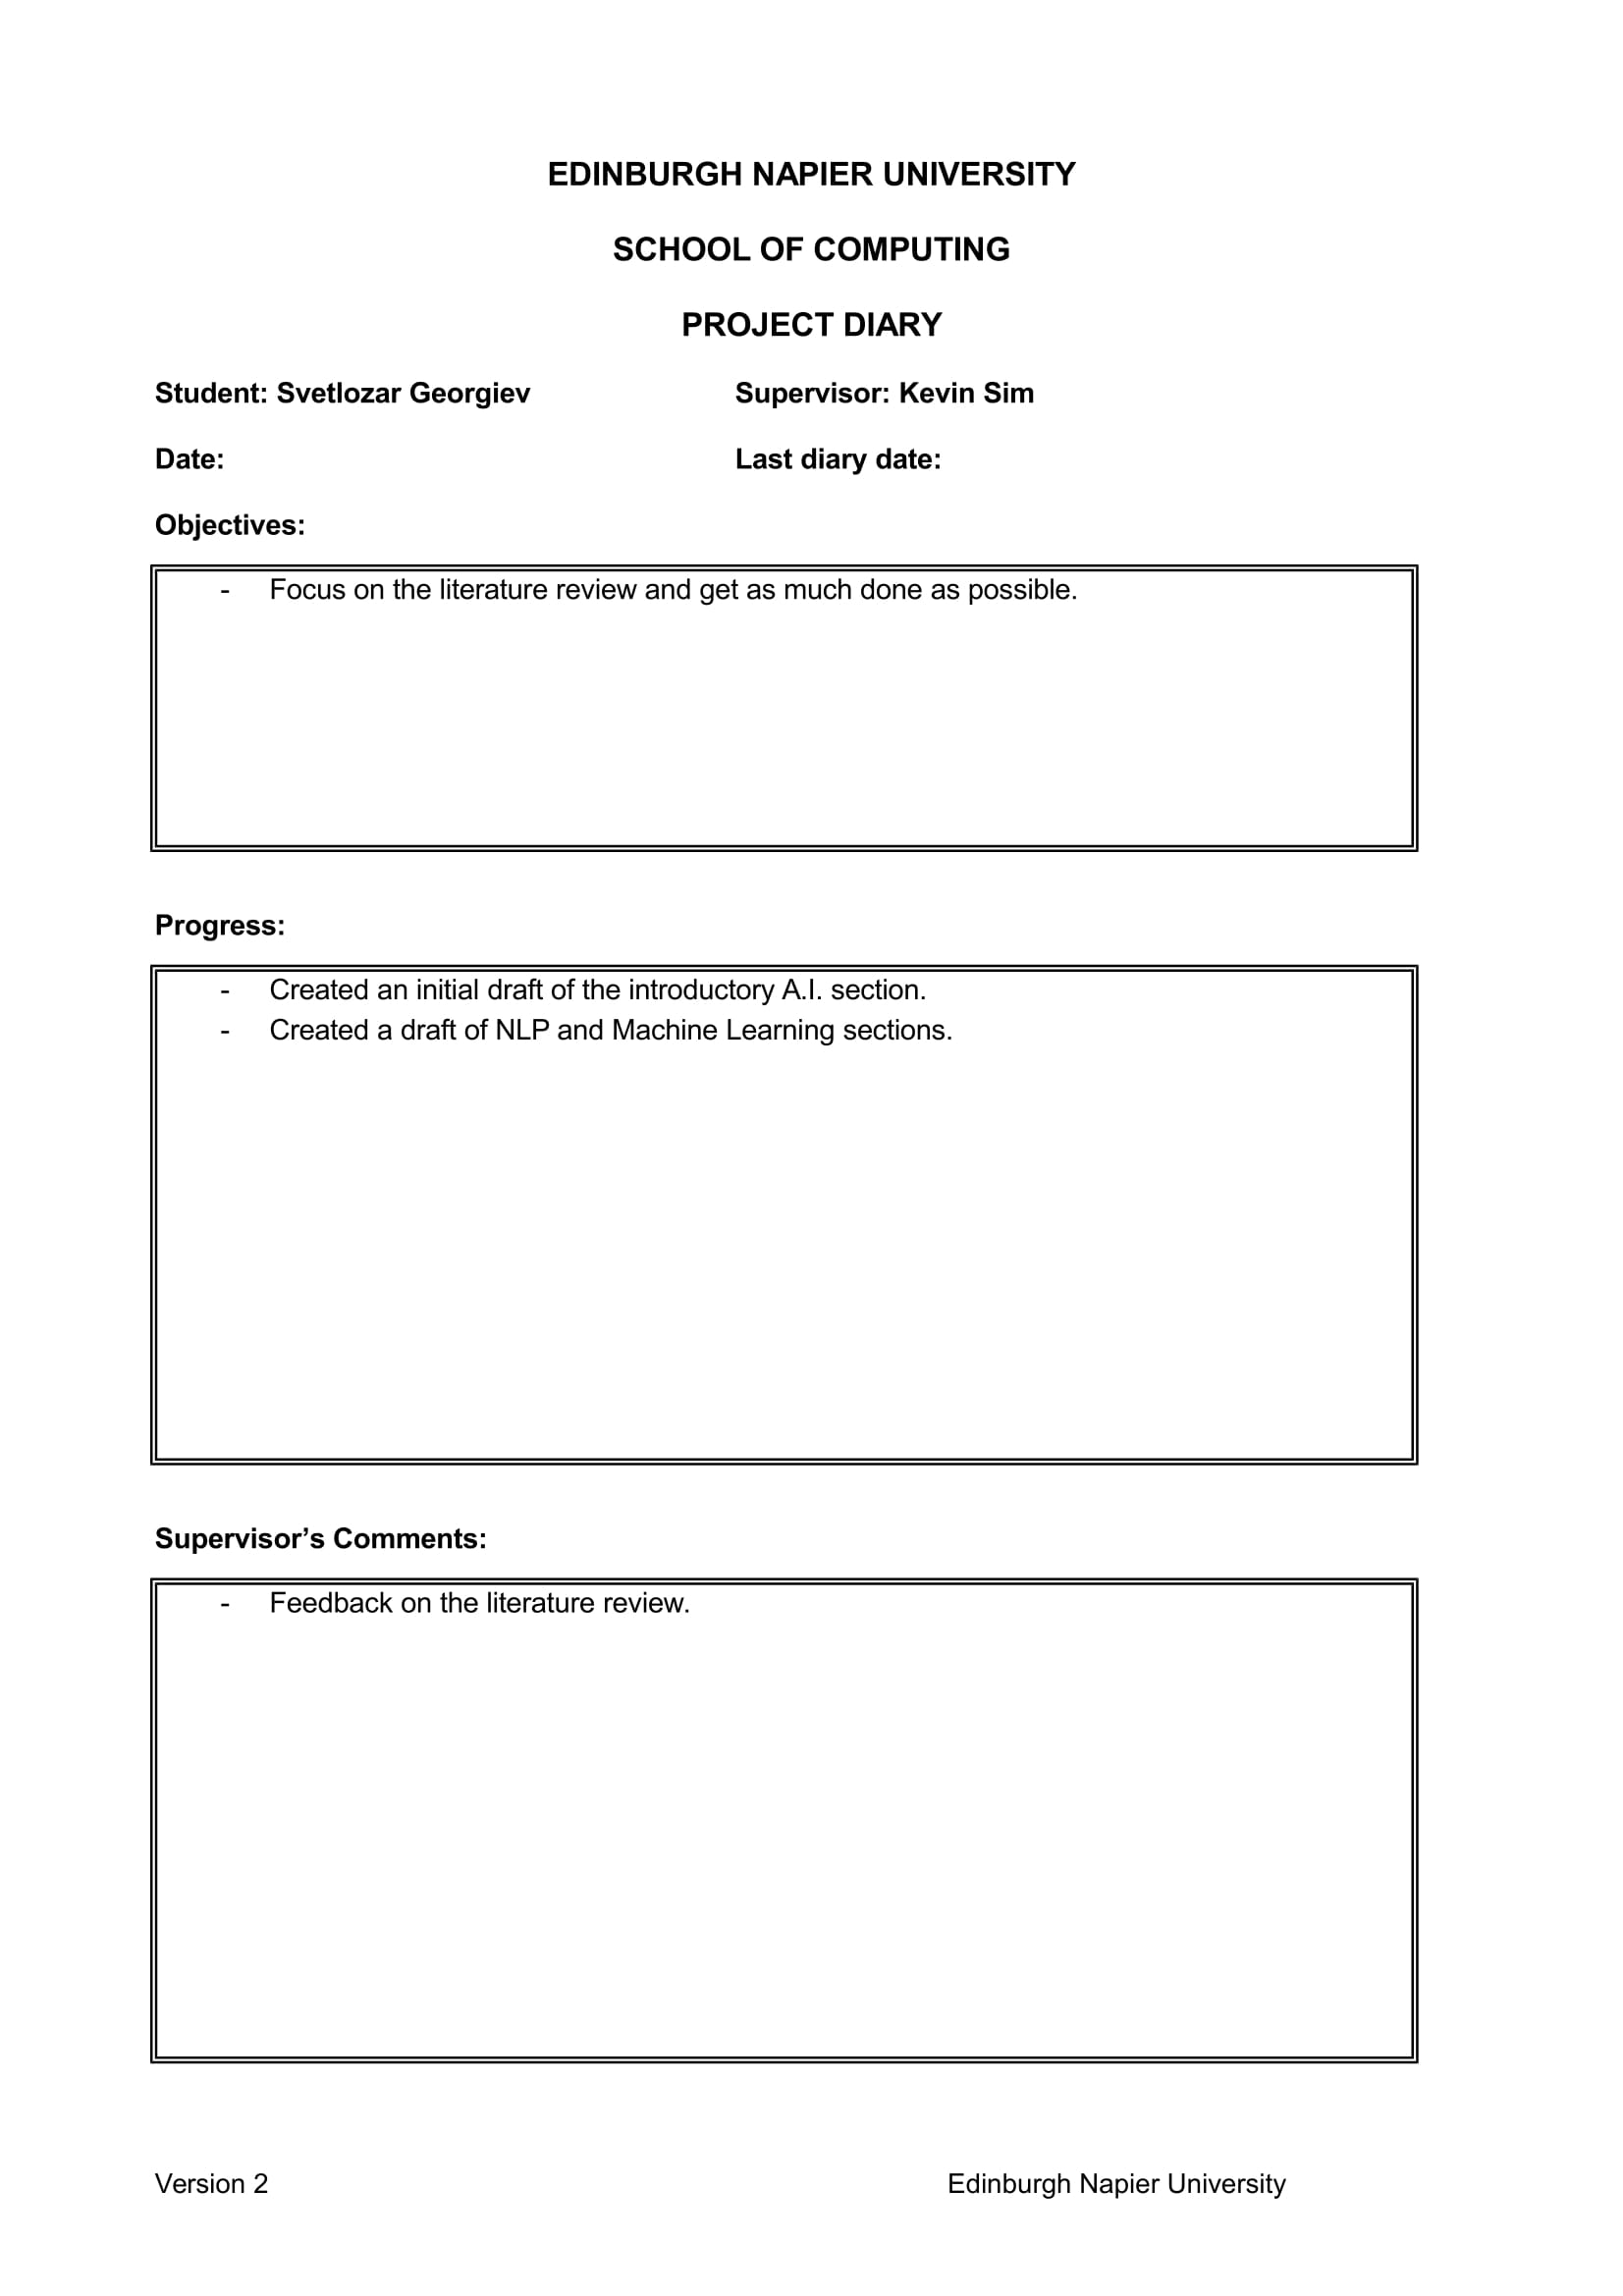
\includegraphics[width=\textwidth,height=\textheight,keepaspectratio]{week8.jpg}
\newpage
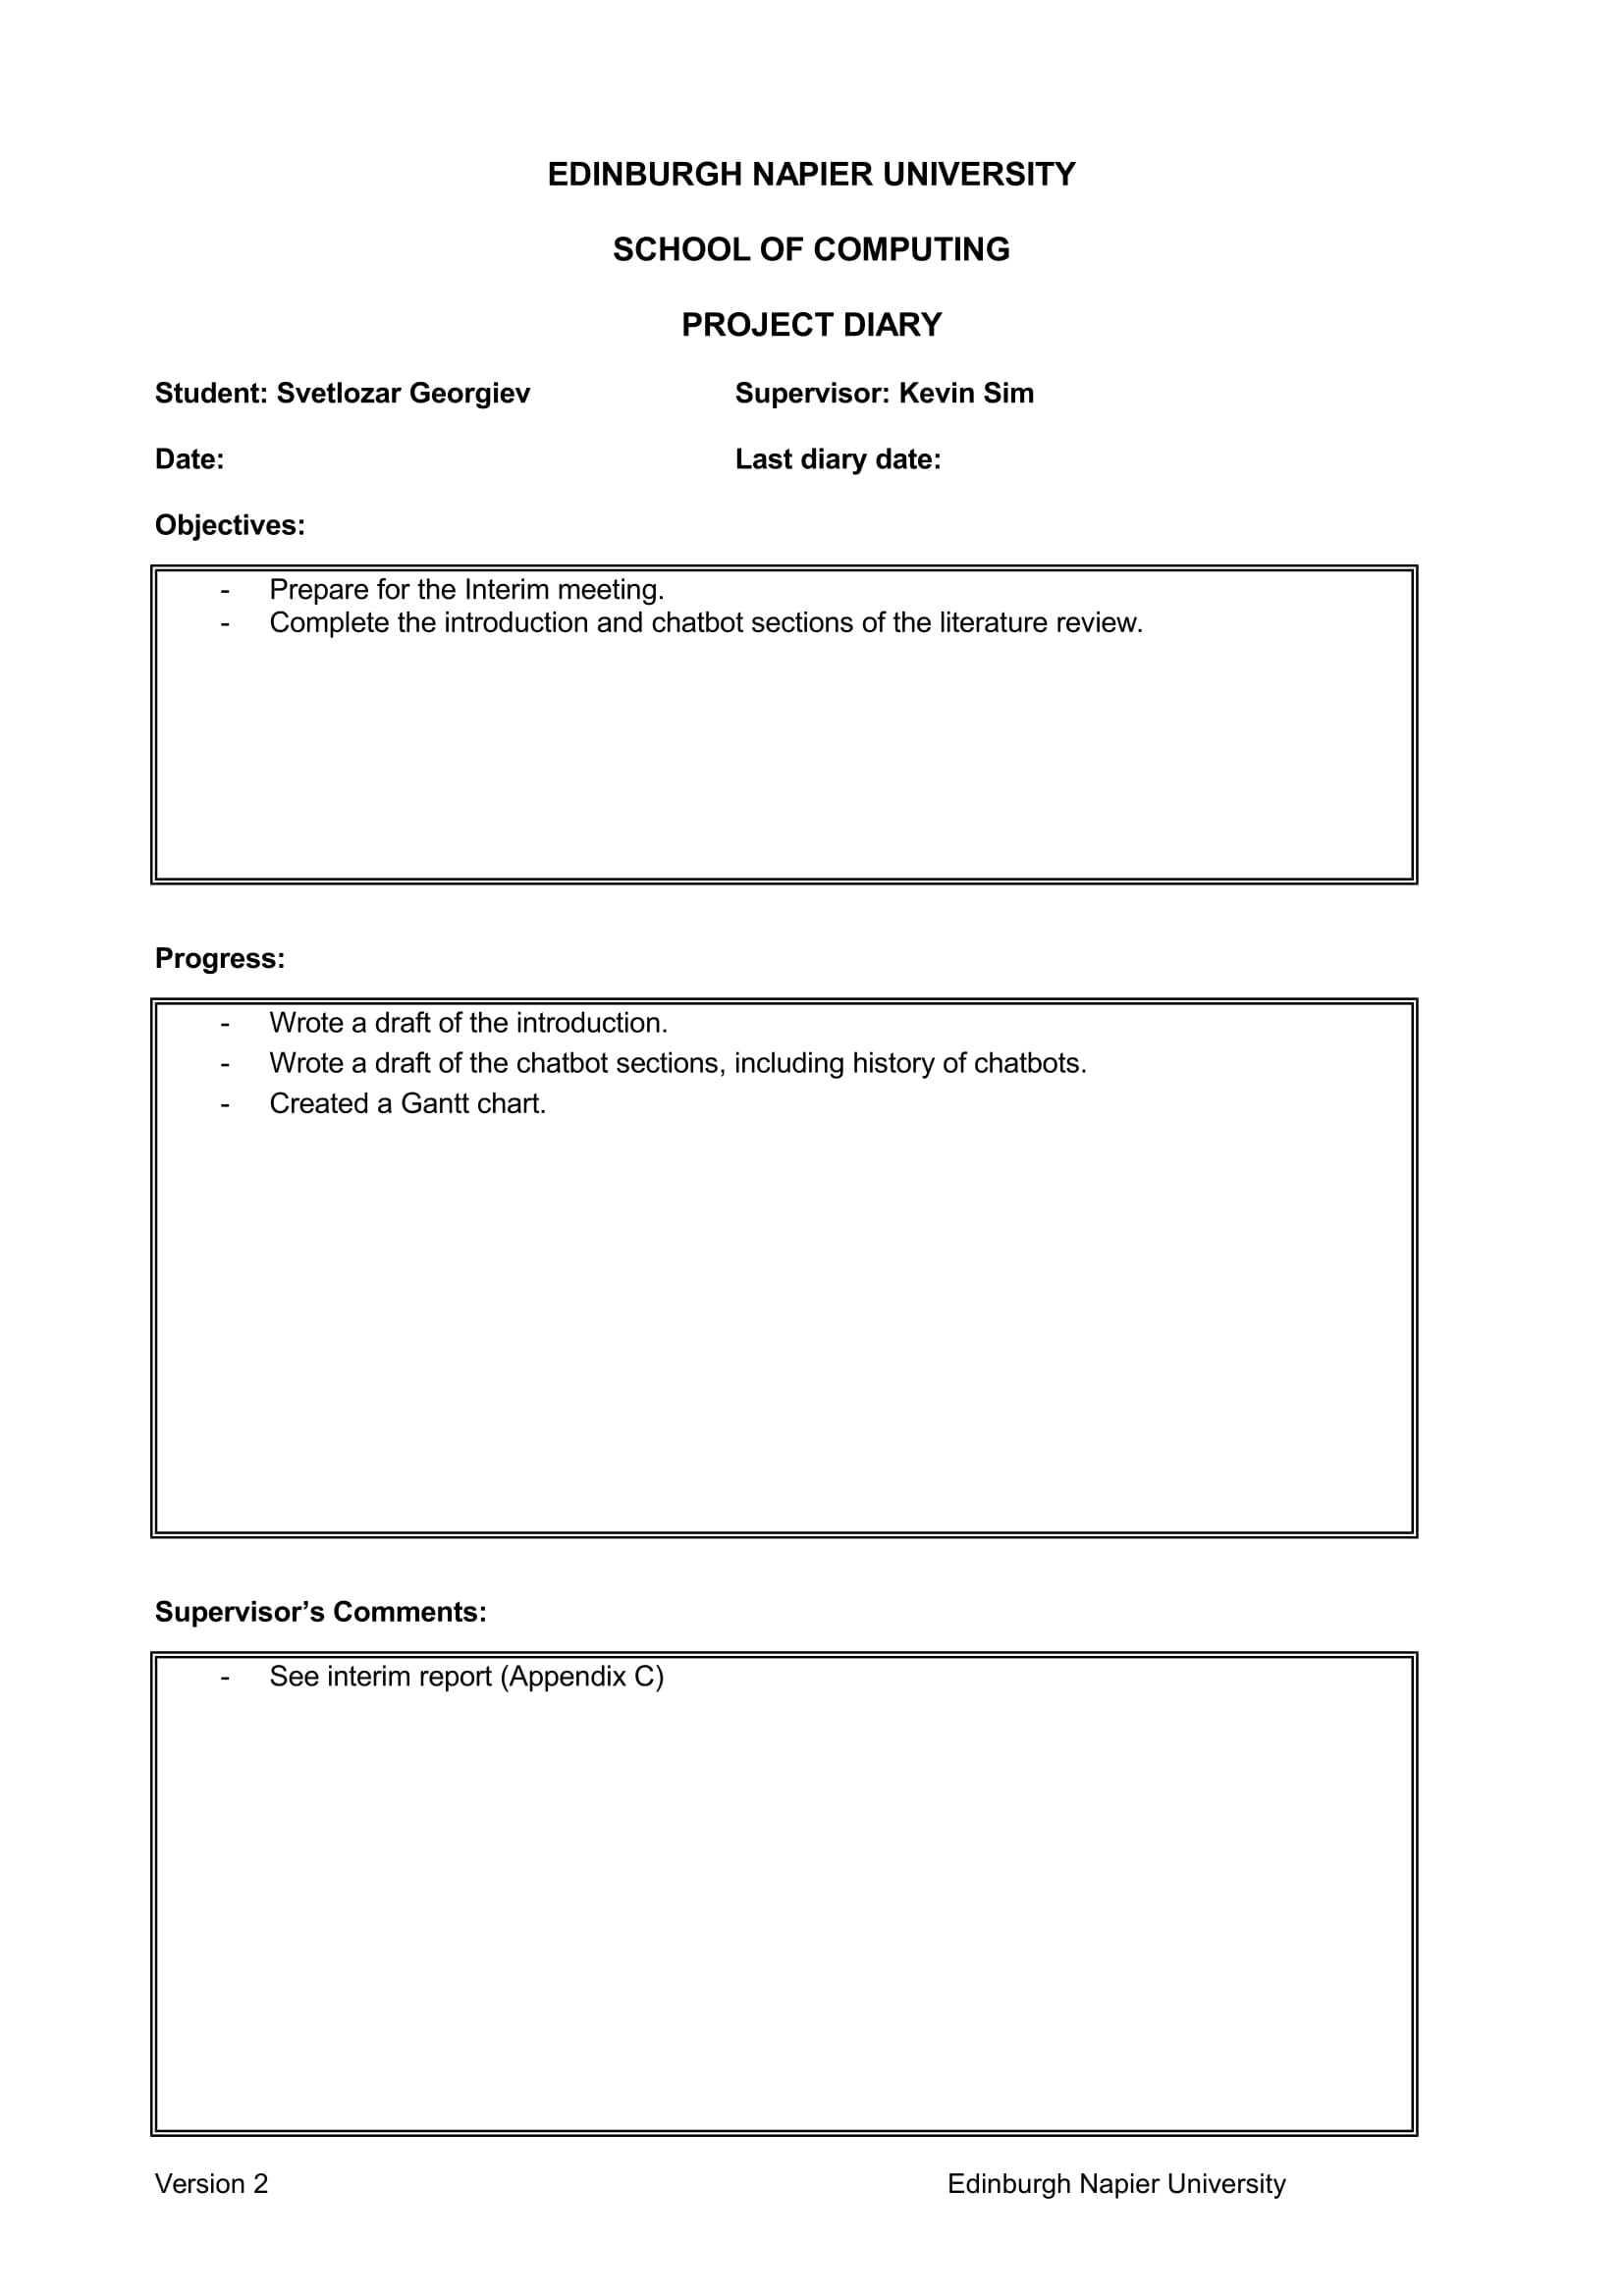
\includegraphics[width=\textwidth,height=\textheight,keepaspectratio]{week9.jpg}
% second semester
% ...
\newpage
\section{Second Formal Review Output}
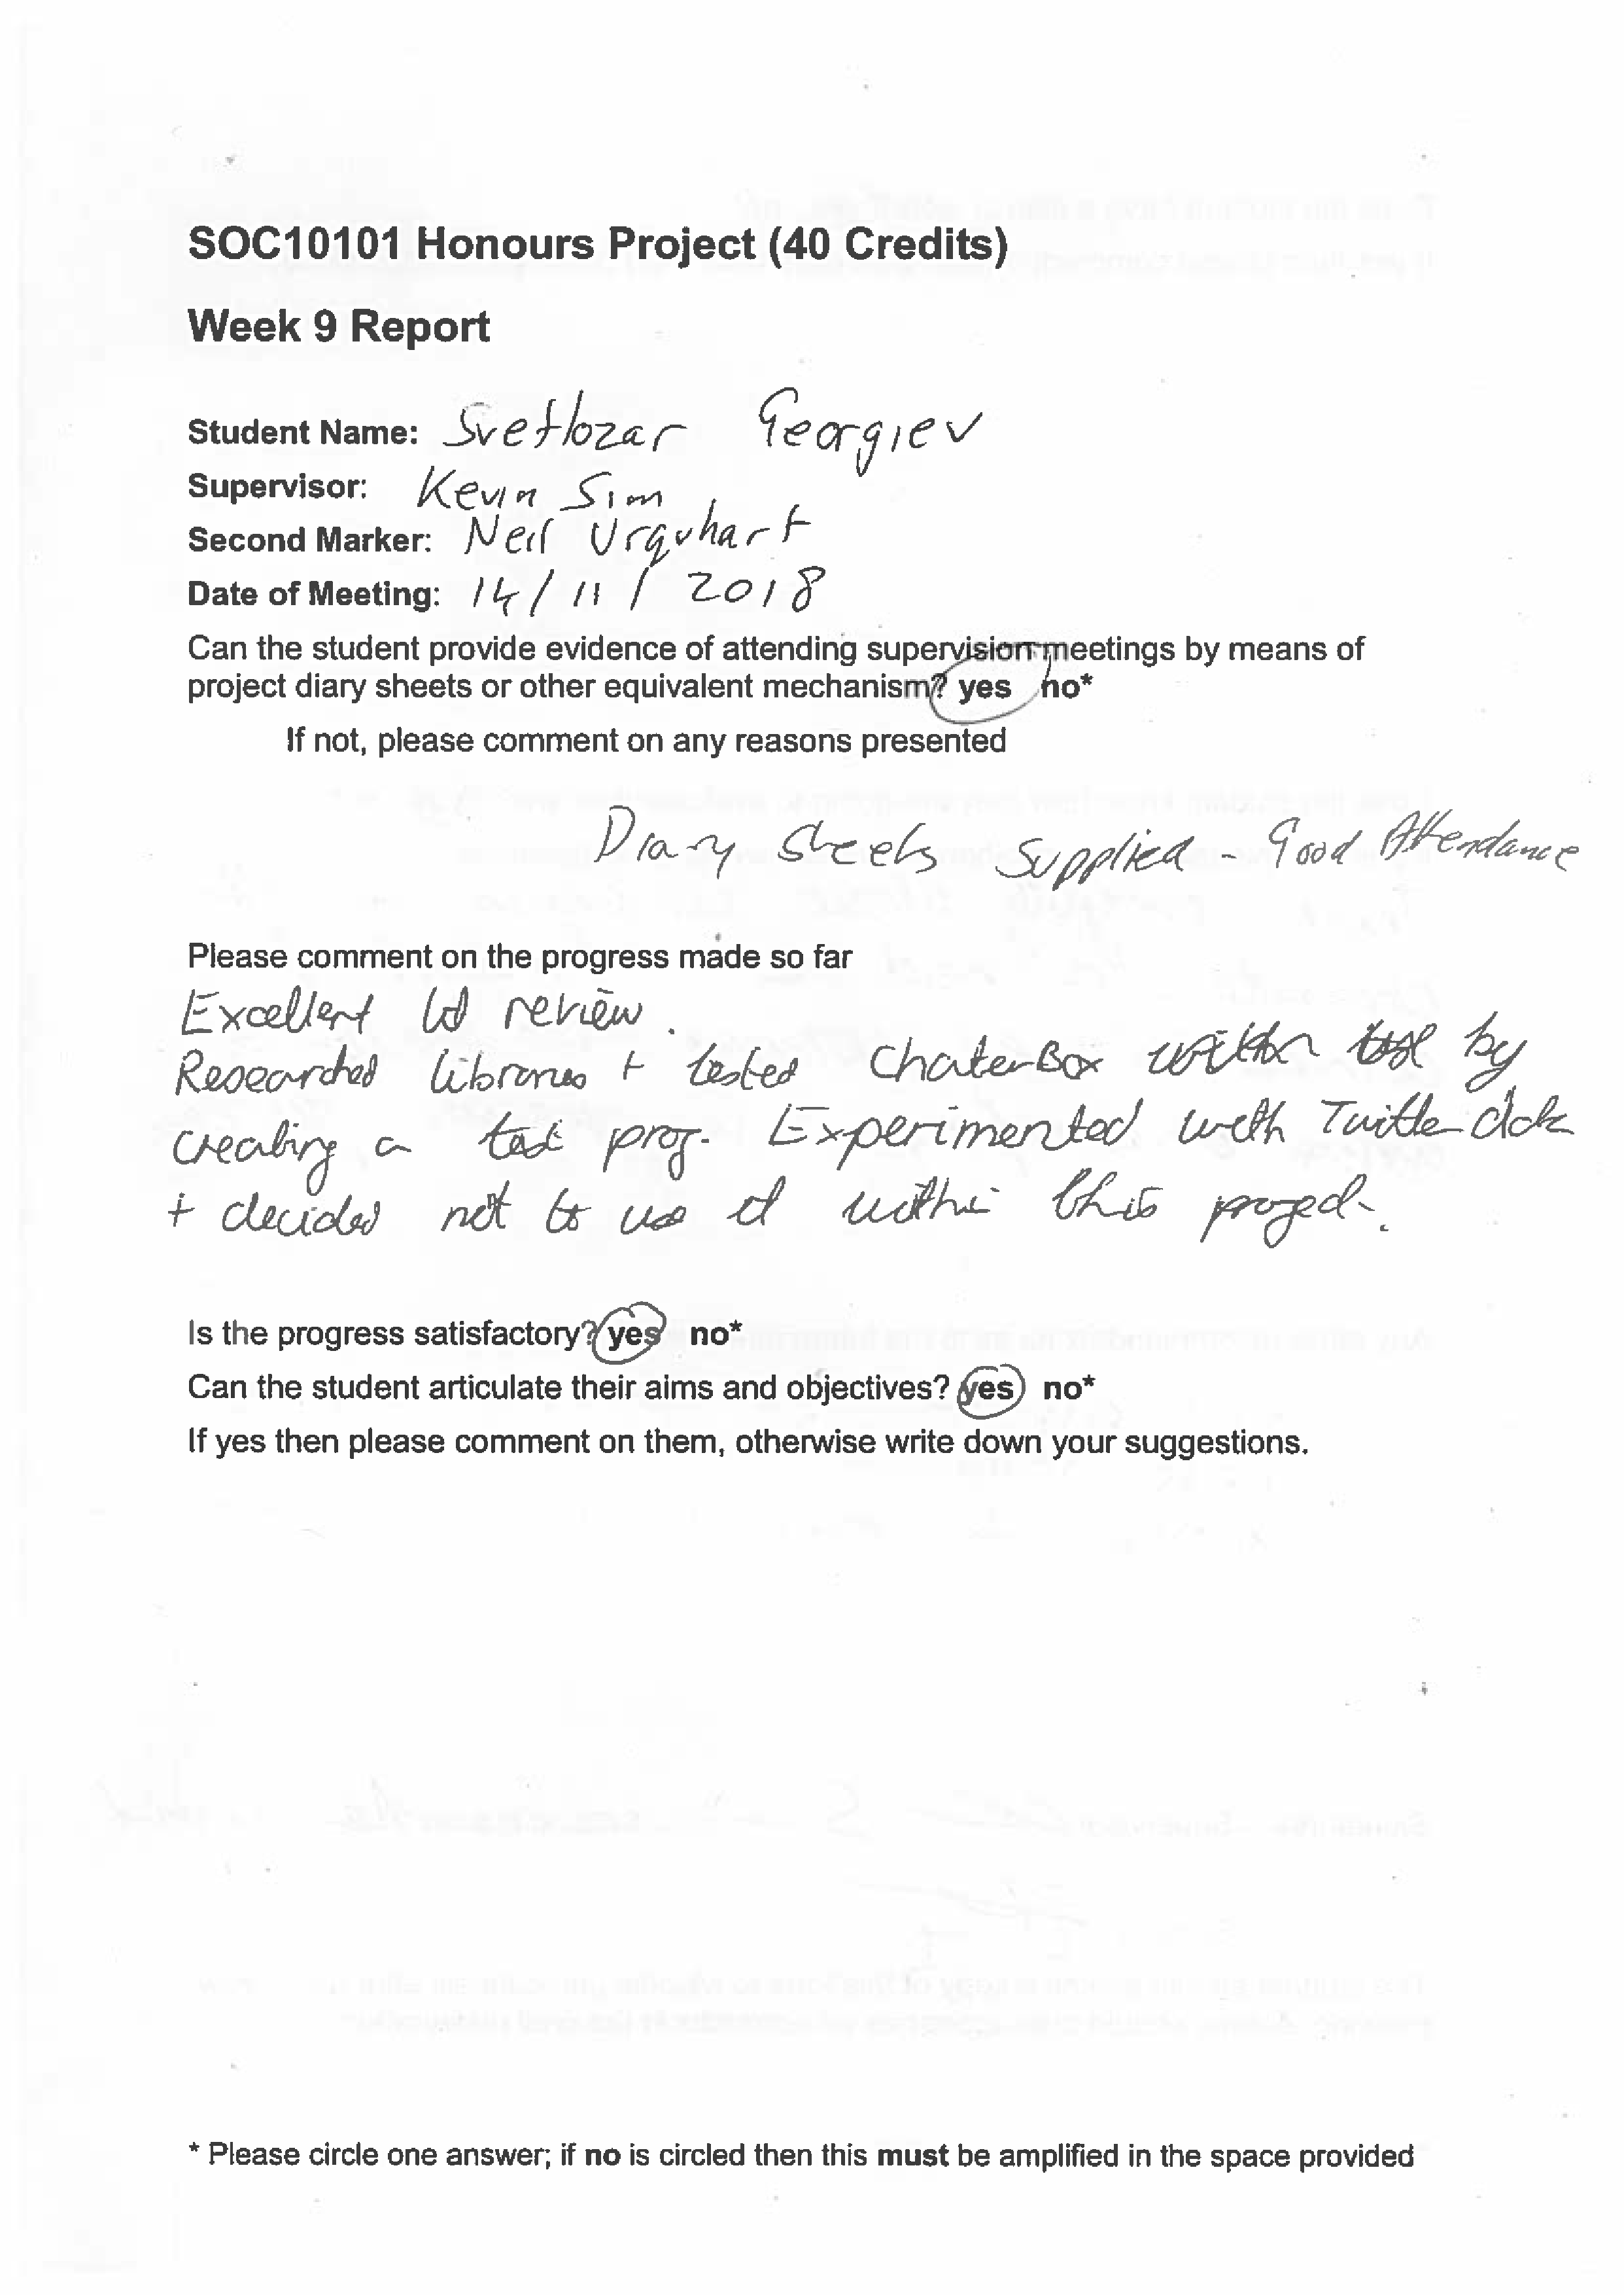
\includegraphics[width=\textwidth,height=\textheight,keepaspectratio]{interim-1.png}
\newpage
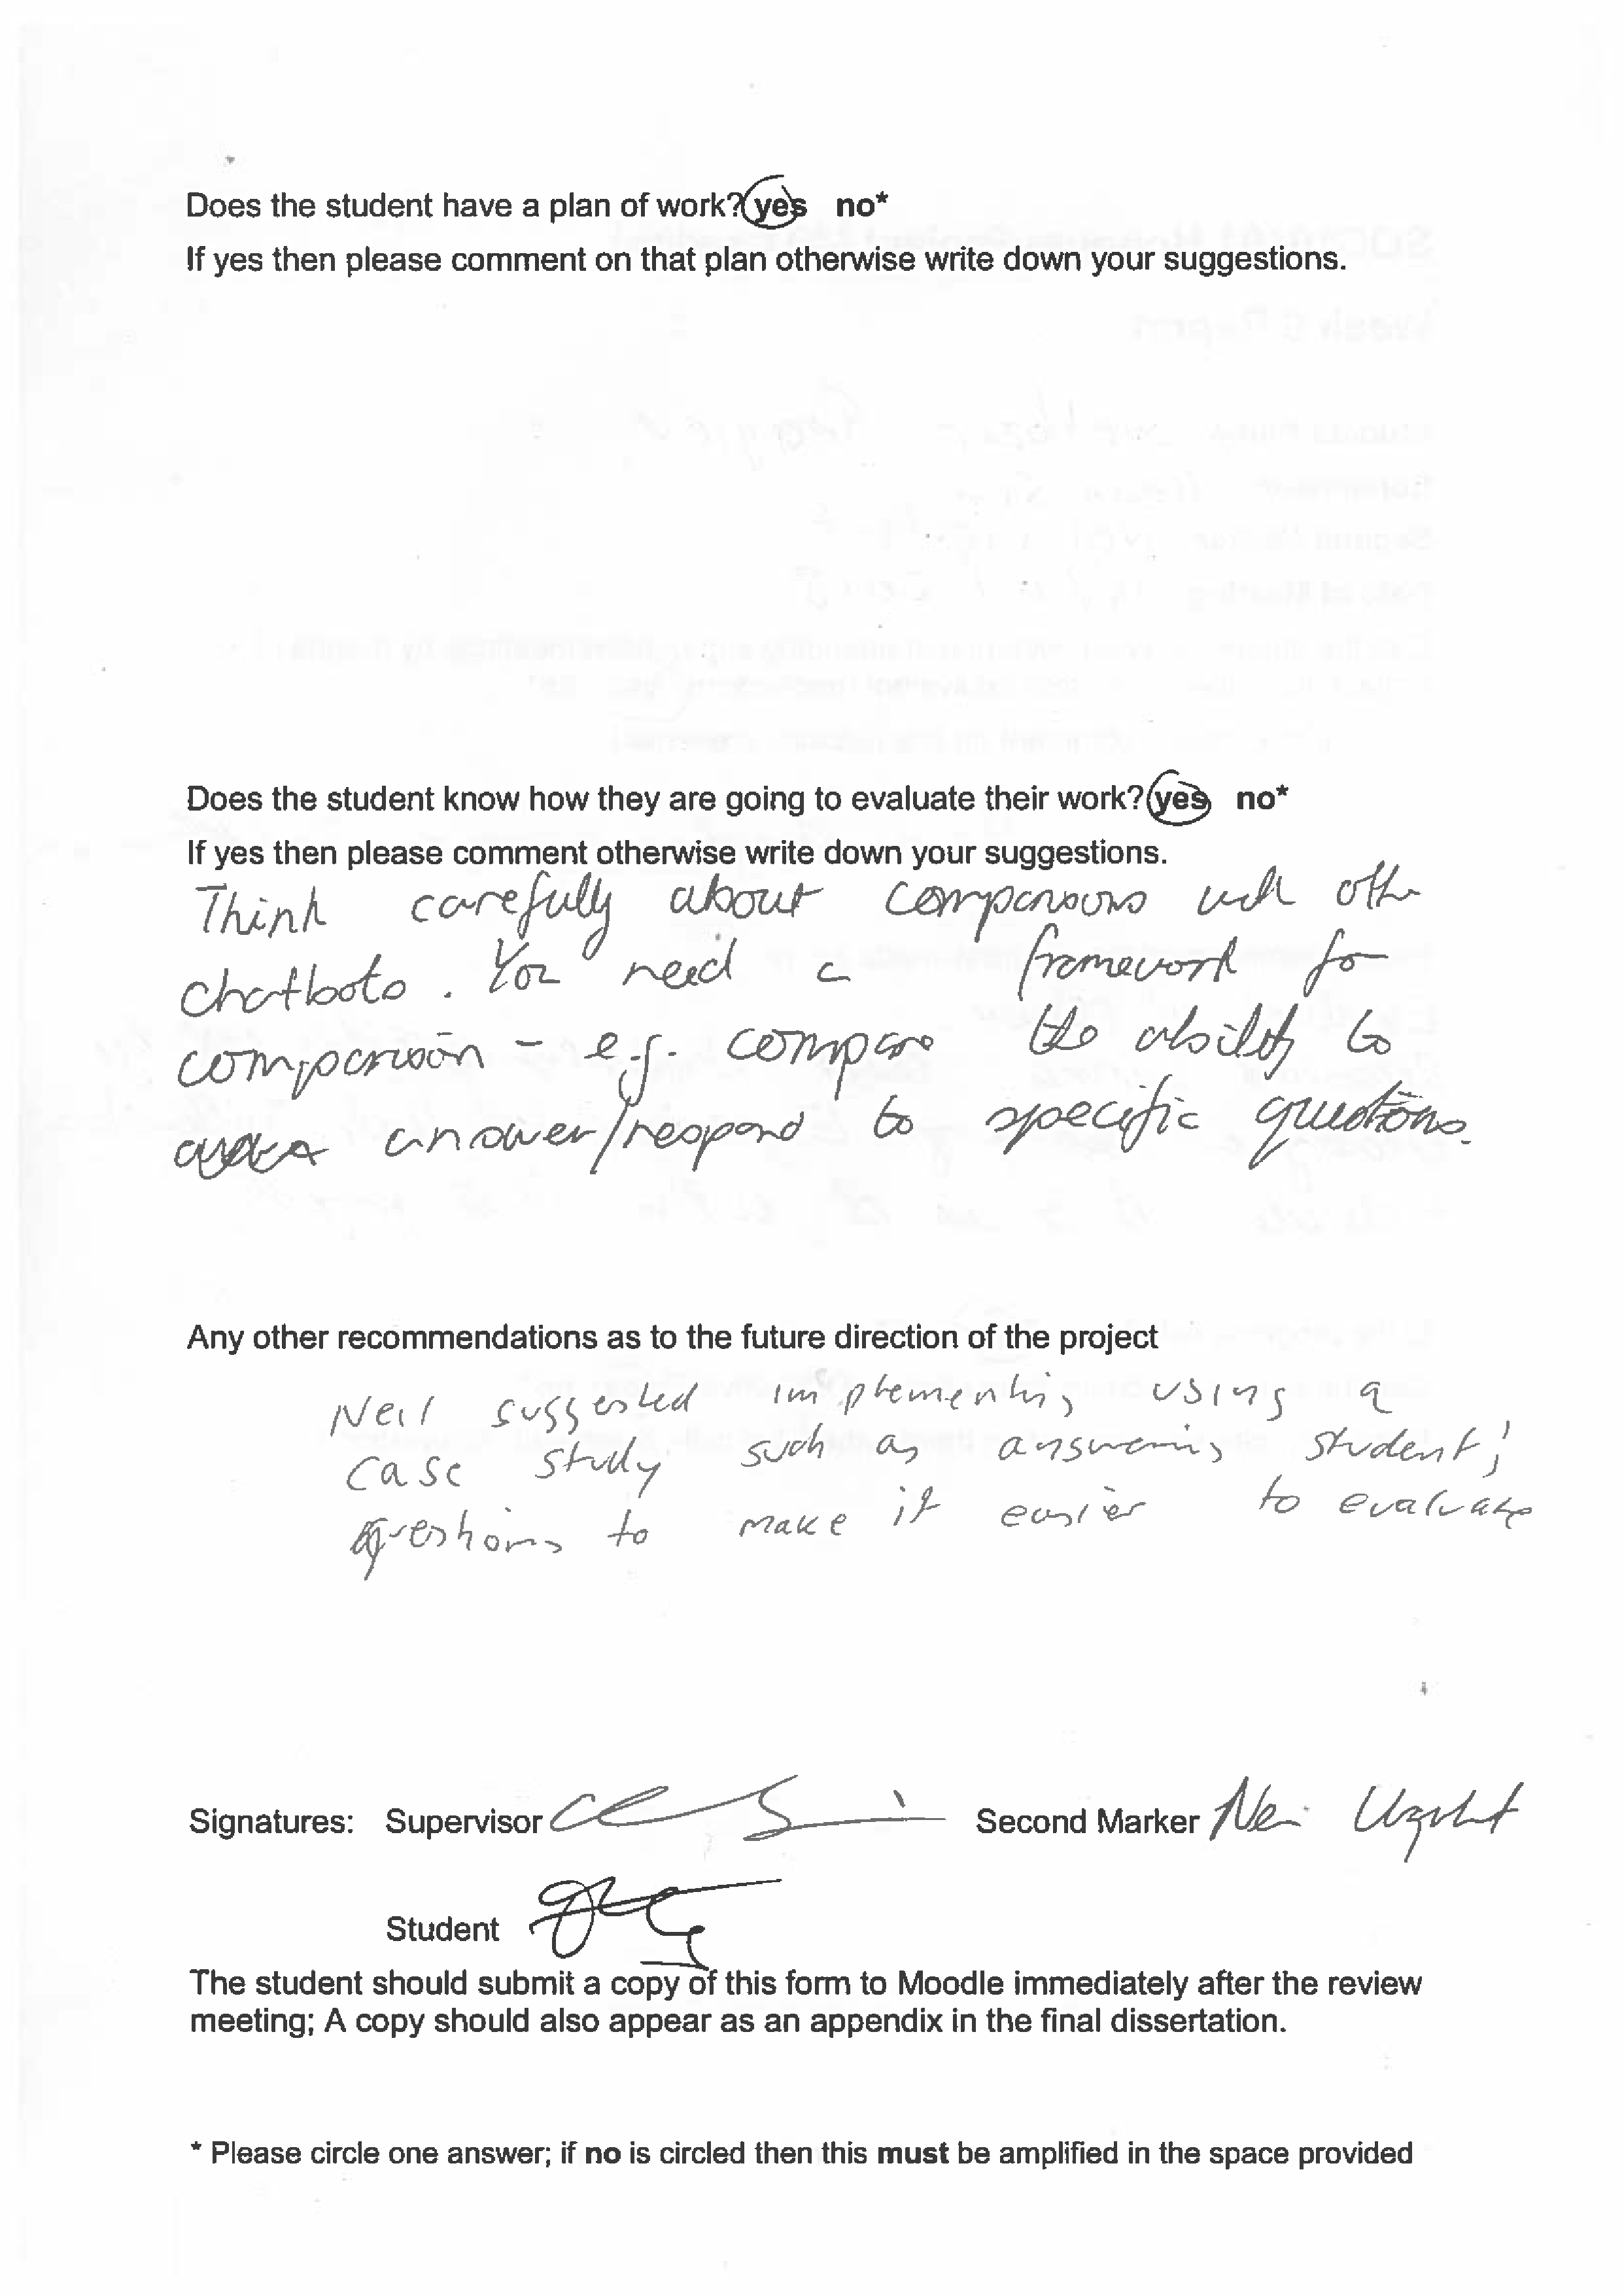
\includegraphics[width=\textwidth,height=\textheight,keepaspectratio]{interim-2.png}

\newpage
\section{Results from First Testing Session}\label{app:sesh1}
\begin{table}[!htb]
    \centering
    \renewcommand\arraystretch{1.6}
    \caption{\captionstyle{Results from the first testing session.}}
    \label{tbl:sesh1}
    \begin{tabularx}{\textwidth}{XX}
    \toprule
    \textbf{Feedback} & \textbf{Changes made}  \\
    \midrule
    Links are not identifiable easily. & The colour of all links was changed to stand out from regular text. The style was also  changed so that they are underlined. \\
    The \enquote{help} link is not visible. & The style for this link was also changed.  Additionally, another help button was added to a menu at the top of the webpage. \\
    It would be more user-friendly to add an "alternate response" button. & An alternate response button was added to the bottom of each bot message.\\
    When the user gives negative feedback, they should be presented with an alternate  response button. & An alternate response button was added to the template for the "no" feedback button. \\
    The webpage fills the screen and  answers which are too long look like a wall of text. It is difficult to read. & The initial width of the chat box was decreased. \\
    The help message should describe the features of the application more clearly. & The help message was edited. \\
    There should be a description of the website for users who accidentally found it. & Another webpage was added which describes the purpose of the website.\\
    \bottomrule
    \end{tabularx}
\end{table}%

\newpage
\section{Survey Questions}\label{app:surveyqs}
\renewcommand\arraystretch{1.8}
\begin{longtabu} to \textwidth {cX[1]X[1]}
    \caption{\captionstyle{The questions each tester was asked in the survey and their possible answers.}} \label{tbl:sureyqs} \\
    \toprule
    \multicolumn{1}{l}{\textbf{ID}} & \multicolumn{1}{l}{\textbf{Question}} & \multicolumn{1}{l}{\textbf{Possible Answers}} \\
    \endfirsthead

    \multicolumn{3}{c}%
    {{\bfseries \tablename\ \thetable{} -- continued from previous page}} \\
    \toprule \multicolumn{1}{l}{\textbf{ID}} & \multicolumn{1}{l}{\textbf{Question}} & \multicolumn{1}{l}{\textbf{Possible Answers}} \\ \hline
    \endhead

    \hline \multicolumn{3}{r}{{\small{Continued on next page}}} \\ \bottomrule 
    \endfoot

    \bottomrule
    \endlastfoot
    
    \midrule
    1 & What year of study are you in? & 1st/2nd/3rd/4th \\
    2 & What is your overall programming knowledge? & Beginner/Intermediate/Advanced \\
    3 & How often do you use search engines to search for information related to programming? & Daily/Weekly/Monthly/Less often\\
    4 & How often do you use Stack Overflow? & Daily/Weekly/Monthly/Less often \\
    5 & The user interface is easy to understand and use. & Scale from "Strongly Agree" to "Strongly Disagree" \\
    6 & The user interface is visually pleasing. & Scale from "Strongly Agree" to "Strongly Disagree" \\
    7 & I was able to understand how to use all the features of the application, i.e. asking for a \textbf{regular response}, asking for an \textbf{alternate response}, and providing \textbf{feedback} for a bot response. & Scale from "Strongly Agree" to "Strongly Disagree" \\
    8 & I was able to use the \textbf{alternate response feature} to receive an alternate answer to a question I asked. & Scale from "Strongly Agree" to "Strongly Disagree".\\
    9 & I was able to use the \textbf{feedback feature} to give feedback on an answer the chatbot gave me. & Scale from "Strongly Agree" to "Strongly Disagree" \\
    10 & Appropriate error messages are shown (e.g. when there is no user input). & Scale from "Strongly Agree" to "Strongly Disagree" \\
    11 & The chatbot answered my question(s) quickly. & Scale from "Strongly Agree" to "Strongly Disagree" \\
    12 & The chatbot response(s) were coherent and answered my question(s) accurately. & Scale from "Strongly Agree" to "Strongly Disagree" \\
    13 & I am overall satisfied with the functionality of the application. & Scale from "Strongly Agree" to "Strongly Disagree" \\
    14 & I prefer using the application on a... & Mobile Device/Desktop Device \\
    15 & Any additional feedback? & Text input field where the user can write their additional feedback.\\
\end{longtabu}


\end{appendices}

\end{document}
